%% History:
% Pavel Tvrdik (26.12.2004)
%  + initial version for PhD Report
%
% Daniel Sykora (27.01.2005)
%
% Michal Valenta (3.12.2008)
% rada zmen ve formatovani (diky M. Duškovi, J. Holubovi a J. Žďárkovi)
% sjednoceni zdrojoveho kodu pro anglickou, ceskou, bakalarskou a diplomovou praci

% One-page layout: (proof-)reading on display
%%%% \documentclass[11pt,oneside,a4paper]{book}
% Two-page layout: final printing
\documentclass[11pt,twoside,a4paper]{book}   
%=-=-=-=-=-=-=-=-=-=-=-=--=%
% The user of this template may find useful to have an alternative to these 
% officially suggested packages:
\usepackage{verbatim}
\usepackage{amsmath, amsthm, amssymb}
\usepackage[czech, english]{babel}
\usepackage[T1]{fontenc} % pouzije EC fonty 
% pripadne pisete-li cesky, pak lze zkusit take:
% \usepackage[OT1]{fontenc} 
\usepackage[utf8]{inputenc}
%=-=-=-=-=-=-=-=-=-=-=-=--=%
% In case of problems with PDF fonts, one may try to uncomment this line:
%\usepackage{lmodern}
%=-=-=-=-=-=-=-=-=-=-=-=--=%
%=-=-=-=-=-=-=-=-=-=-=-=--=%
% Depending on your particular TeX distribution and version of conversion tools 
% (dvips/dvipdf/ps2pdf), some (advanced | desperate) users may prefer to use 
% different settings.
% Please uncomment the following style and use your CSLaTeX (cslatex/pdfcslatex) 
% to process your work. Note however, this file is in UTF-8 and a conversion to 
% your native encoding may be required. Some settings below depend on babel 
% macros and should also be modified. See \selectlanguage \iflanguage.
%\usepackage{czech}  %%%%%\usepackage[T1]{czech} %%%%[IL2] [T1] [OT1]
%=-=-=-=-=-=-=-=-=-=-=-=--=%

%%%%%%%%%%%%%%%%%%%%%%%%%%%%%%%%%%%%%%%
% Styles required in your work follow %
%%%%%%%%%%%%%%%%%%%%%%%%%%%%%%%%%%%%%%%
\usepackage{graphicx}
%\usepackage{indentfirst} %1. odstavec jako v cestine.

\usepackage{k336_thesis_macros} % specialni makra pro formatovani DP a BP
 % muzete si vytvorit i sva vlastni v souboru k336_thesis_macros.sty
 % najdete  radu jednoduchych definic, ktere zde ani nejsou pouzity
 % napriklad: 
 % \newcommand{\bfig}{\begin{figure}\begin{center}}
 % \newcommand{\efig}{\end{center}\end{figure}}
 % umoznuje pouzit prikaz \bfig namisto \begin{figure}\begin{center} atd.


%%%%%%%%%%%%%%%%%%%%%%%%%%%%%%%%%%%%%
% Zvolte jednu z moznosti 
% Choose one of the following options
%%%%%%%%%%%%%%%%%%%%%%%%%%%%%%%%%%%%%
\newcommand\TypeOfWork{Diplomová práce} \typeout{Diplomova prace}
% \newcommand\TypeOfWork{Master's Thesis}   \typeout{Master's Thesis} 
% \newcommand\TypeOfWork{Bakalářská práce}  \typeout{Bakalarska prace}
% \newcommand\TypeOfWork{Bachelor's Project}  \typeout{Bachelor's Project}


%%%%%%%%%%%%%%%%%%%%%%%%%%%%%%%%%%%%%
% Zvolte jednu z moznosti 
% Choose one of the following options
%%%%%%%%%%%%%%%%%%%%%%%%%%%%%%%%%%%%%
% nabidky jsou z: http://www.fel.cvut.cz/cz/education/bk/prehled.html

%\newcommand\StudProgram{Elektrotechnika a informatika, dobíhající, Bakalářský}
%\newcommand\StudProgram{Elektrotechnika a informatika, dobíhající, Magisterský}
% \newcommand\StudProgram{Elektrotechnika a informatika, strukturovaný, Bakalářský}
 \newcommand\StudProgram{Otevřená informatika, strukturovaný, Navazující magisterský}
% \newcommand\StudProgram{Softwarové technologie a management, Bakalářský}
% English study:
% \newcommand\StudProgram{Electrical Engineering and Information Technology}  % bachelor programe
% \newcommand\StudProgram{Electrical Engineering and Information Technology}  %master program


%%%%%%%%%%%%%%%%%%%%%%%%%%%%%%%%%%%%%
% Zvolte jednu z moznosti 
% Choose one of the following options
%%%%%%%%%%%%%%%%%%%%%%%%%%%%%%%%%%%%%
% nabidky jsou z: http://www.fel.cvut.cz/cz/education/bk/prehled.html

%\newcommand\StudBranch{Výpočetní technika}   % pro program EaI bak. (dobihajici i strukt.)
\newcommand\StudBranch{Počítačová grafika a interakce}   % pro program OI mag. (strukt.)
%\newcommand\StudBranch{Softwarové inženýrství}            %pro STM
%\newcommand\StudBranch{Web a multimedia}                  % pro STM
%\newcommand\StudBranch{Computer Engineering}              % bachelor programe
%\newcommand\StudBranch{Computer Science and Engineering}  % master programe


%%%%%%%%%%%%%%%%%%%%%%%%%%%%%%%%%%%%%%%%%%%%
% Vyplnte nazev prace, autora a vedouciho
% Set up Work Title, Author and Supervisor
%%%%%%%%%%%%%%%%%%%%%%%%%%%%%%%%%%%%%%%%%%%%

\newcommand\WorkTitle{Realistické zobrazování modelů vegetace v reálném čase}
\newcommand\FirstandFamilyName{Bc. Adam Kučera}
\newcommand\Supervisor{Ing. Jiří Bittner, PhD.}


\newcommand{\lineCode}[1]{\mbox{\texttt{#1}}}

% Pouzijete-li pdflatex, tak je prijemne, kdyz bude mit vase prace
% funkcni odkazy i v pdf formatu
\usepackage[
pdftitle={\WorkTitle},
pdfauthor={\FirstandFamilyName},
bookmarks=true,
colorlinks=true,
breaklinks=true,
urlcolor=black,
citecolor= blue,
linkcolor= black,
unicode=true,
]
{hyperref}



% Extension posted by Petr Dlouhy in order for better sources reference (\cite{} command) especially in Czech.
% April 2010
% See comment over \thebibliography command for details.

\usepackage[square, numbers]{natbib}             % sazba pouzite literatury
%\usepackage{url}
%\DeclareUrlCommand\url{\def\UrlLeft{<}\def\UrlRight{>}\urlstyle{tt}}  %rm/sf/tt
%\renewcommand{\emph}[1]{\textsl{#1}}    % melo by byt kurziva nebo sklonene,
\let\oldUrl\url
\renewcommand\url[1]{<\texttt{\oldUrl{#1}}>}




\begin{document}

%%%%%%%%%%%%%%%%%%%%%%%%%%%%%%%%%%%%%
% Zvolte jednu z moznosti 
% Choose one of the following options
%%%%%%%%%%%%%%%%%%%%%%%%%%%%%%%%%%%%%
\selectlanguage{czech}
%\selectlanguage{english} 

% prikaz \typeout vypise vyse uvedena nastaveni v prikazovem okne
% pro pohodlne ladeni prace


\iflanguage{czech}{
	 \typeout{************************************************}
	 \typeout{Zvoleny jazyk: cestina}
	 \typeout{Typ prace: \TypeOfWork}
	 \typeout{Studijni program: \StudProgram}
	 \typeout{Obor: \StudBranch}
	 \typeout{Jmeno: \FirstandFamilyName}
	 \typeout{Nazev prace: \WorkTitle}
	 \typeout{Vedouci prace: \Supervisor}
	 \typeout{***************************************************}
	 \newcommand\Department{Katedra počítačů}
	 \newcommand\Faculty{Fakulta elektrotechnická}
	 \newcommand\University{České vysoké učení technické v Praze}
	 \newcommand\labelSupervisor{Vedoucí práce}
	 \newcommand\labelStudProgram{Studijní program}
	 \newcommand\labelStudBranch{Obor}
}{
	 \typeout{************************************************}
	 \typeout{Language: english}
	 \typeout{Type of Work: \TypeOfWork}
	 \typeout{Study Program: \StudProgram}
	 \typeout{Study Branch: \StudBranch}
	 \typeout{Author: \FirstandFamilyName}
	 \typeout{Title: \WorkTitle}
	 \typeout{Supervisor: \Supervisor}
	 \typeout{***************************************************}
	 \newcommand\Department{Department of Computer Science and Engineering}
	 \newcommand\Faculty{Faculty of Electrical Engineering}
	 \newcommand\University{Czech Technical University in Prague}
	 \newcommand\labelSupervisor{Supervisor}
	 \newcommand\labelStudProgram{Study Programme} 
	 \newcommand\labelStudBranch{Field of Study}
}




%%%%%%%%%%%%%%%%%%%%%%%%%%    Poznamky ke kompletaci prace
% Nasledujici pasaz uzavrenou v {} ve sve praci samozrejme 
% zakomentujte nebo odstrante. 
% Ve vysledne svazane praci bude nahrazena skutecnym 
% oficialnim zadanim vasi prace.
{
\pagenumbering{roman} \cleardoublepage \thispagestyle{empty}
\chapter*{Na tomto místě bude oficiální zadání práce}
\begin{comment}
	\begin{itemize}
		\item čeština funguje? ňďťěščřžýáíéúů ŇĎŤĚŠČŘŽÝÁÍÉÚŮ,
		\item musíte si ho vyzvednout na studiijním oddělení Katedry počítačů na Karlově náměstí,
		\item v jedné odevzdané práci bude originál tohoto zadání (originál zůstává po obhajobě na katedře),
		\item ve druhé bude na stejném místě neověřená kopie tohoto dokumentu (tato se vám vrátí po obhajobě).
	\end{itemize}
\end{comment}
\newpage
}

%%%%%%%%%%%%%%%%%%%%%%%%%%    Titulni stranka / Title page 

\coverpagestarts

%%%%%%%%%%%%%%%%%%%%%%%%%%%    Podekovani / Acknowledgements 

\acknowledgements
\noindent
Velice rád bych touto cestou poděkoval vedoucímu práce Ing. Jiřímu Bittnerovi, PhD. za podnětné vedení práce.
\newline I would also like to express my thanks to Ralf Habel for inspiring consultations and providing advanced leaf texture data.



%%%%%%%%%%%%%%%%%%%%%%%%%%%   Prohlaseni / Declaration 

\declaration{V~Liberci dne \today}


%%%%%%%%%%%%%%%%%%%%%%%%%%%%    Abstract 
 
\abstractpage

Translation of Czech abstract into English.

% Prace v cestine musi krome abstraktu v anglictine obsahovat i
% abstrakt v cestine.
\vglue60mm

\noindent{\Huge \textbf{Abstrakt}}
\vskip 2.75\baselineskip

\noindent
Abstrakt v češtině

\noindent
Očekávají se cca 1 -- 2 odstavce, maximálně půl stránky.

%%%%%%%%%%%%%%%%%%%%%%%%%%%%%%%%  Obsah / Table of Contents 

\tableofcontents


%**************************************************************

\mainbodystarts
% horizontalní mezera mezi dvema odstavci
%\parskip=5pt
%11.12.2008 parskip + tolerance
\normalfont
\parskip=0.2\baselineskip plus 0.2\baselineskip minus 0.1\baselineskip

% Odsazeni prvniho radku odstavce resi class book (neaplikuje se na prvni 
% odstavce kapitol, sekci, podsekci atd.) Viz usepackage{indentfirst}.
% Chcete-li selektivne zamezit odsazeni 1. radku nektereho odstavce,
% pouzijte prikaz \noindent.

%**************************************************************

% Pro snadnejsi praci s vetsimi texty je rozumne tyto rozdelit
% do samostatnych souboru nejlepe dle kapitol a tyto potom vkladat
% pomoci prikazu \include{jmeno_souboru.tex} nebo \include{jmeno_souboru}.
% Napr.:
% \include{1_uvod}
% \include{2_teorie}
% atd...

%*ÚVOD****************************************************************************
\chapter{Úvod}
Jedním z cílů oboru počítačové grafiky je vytvářet tak realistický obraz, jak je to jen možné. Takový úkol má ovšem vždy dvě hlediska: jak dobře je známa teorie popisující zobrazovaný jev a jak je možné tuto teorii využít v praxi. Omezení ze strany hardwaru či jiné požadavky (např. časová / paměťová náročnost) pak mohou učinit úlohu velmi těžkou i pro jevy z teoretického hlediska lehce popsatelné. Složitost vizualizace (kromě jiných) silně závisí na složitosti zobrazované scény. 
Zobrazování venkovních scén s velkým množstvím vegetace je považováno za obtížnou úlohu počítačové grafiky, právě kvůli vysoké složitosti takových scén. Věrné real-time renderování každého stébla trávy a každého listu stromu až do nejmenších detailů je na současném hardware nerealizovatelné, pokud ovšem nepřipustíme určitou relaxaci problému. V real-time počítačové grafice je třeba občas rezignovat na dokonalé zobrazení přesně podle příslušné teorie. V takovém případě se požaduje, aby přibližný výsledek byl i přesto velmi podobný přesnému řešení a pozorovatel pokud možno rozdíl nepoznal. Naštěstí existují metody, které zachovávají přijatelnou kvalitu a výrazně snižují nároky na výkon. Jedna z nejvýznamnějších skupin technik vychází z faktu, že detail zobrazeného objektu je limitován svou zobrazenou velikostí na výstupním zařízení. Díky konečnému (a vcelku nízkému) rozlišení obrazovky se zobrazí některé detaily do velikosti pod prahem definovaným Nyquist-Shannonovým vzorkovacím teorémem a mohou proto být vypuštěny. To může značně snížit složitost scény. Další zjednodušení scény lze zavést na základě vlastností lidského vnímání. Některé části scény mají malý vliv na celkový vjem pozorovatele. V rámci takových částí je možné lišit se od exaktního řešení i velmi podstatně aniž by se dojem pozorovatele výrazně zhoršil. Metoda řízení úrovně detailu (Level Of Detail - LOD) využívá právě těchto poznatků.
Se vzrůstajícím výkonem výpočetní techniky vzrůstají i požadavky na kvalitu zobrazování. Nepřekvapí tak, že zobrazení pouhého statického stromu již nevyvolává v uživatelích takový dojem realističnosti, jako vykreslení stromu, který se hýbe vlivem působícího větru. Zohledněním dalšího rozměru problému zobrazování vegetace, kterým je čas, se úloha stane ještě složitější.


%*Popis problému, specifikace cíle****************************************************************************
\chapter{Popis problému, specifikace cíle}
\label{chap:cile}


Jak je již předesláno v předchozí kapitole, komplexní objekty, jako je právě například vegetace, představují v oboru počítačové grafiky zvláštní kategorii s relativně vysokou složitostí jejich zpracování. Celá úloha se řádově komplikuje, požadujeme-li zobrazování v reálném čase. Problém zobrazování vegetace lze mírně abstrahovat na úlohu zobrazování stromů. S vývojem hardwaru a aplikací, které umožňují uživateli interakci s virtuálním prostředím, se zvyšují požadavky na realističnost zobrazované vegetace. Je vyžadováno nejen věrné zobrazení statického stromu, ale také jeho animace. Uvědomíme-li si však, že průměrně rostlý listnatý strom může mít až miliony jednotlivých listů a uživatel požaduje zobrazení ne jednoho stromu, ale hned celého lesa o několika tisících stromů, je přímý a naivní přístup k řešení problému příliš náročný pro současný běžný hardware. Přitom se jedná pouze o prostředí, které dotváří scénu a má významově nižší prioritu než objekty zájmu uživatele (budovy, vozidla, speciální efekty, ostatní hráči - příklady ze světa počítačových her) a tedy by jeho zpracování a zobrazování nemělo vytěžovat ve větší míře dostupné prostředky počítače.
	V následující sekci budou vytyčeny cíle této práce a definována úroveň podrobnosti, které se chce práce přiblížit. Následující text se zaměří na rešerši aktuálního stavu v oblasti real-time renderování vegetace pro vymezenou úroveň podrobnosti. V další kapitole (~\nameref{chap:analyza} ) bude rozpracován teoretický základ pro implementaci softwaru zobrazujícím vegetaci v reálném čase. Kapitola ~\nameref{chap:realizace} popíše specifika výsledné implementace a řešení postatných problémů vyplývajících z její realizace. Ověření a zhodnocení kvalit vytvořeného software se bude věnovat kapitola  ~\nameref{chap:testovani}. Poslední kapitola diskutuje výsledky práce a nastíní možné způsoby vylepšení výsledné implementace.

%%%%%%%%%%%%%%%%%%%%%%%%%%%%%%%%%%%%%%%%%%%%%%%%%%%%%%%%%%%%%%%%%%%%
\section{Vymezení cílů}
Hned na úvod je třeba vyjasnit, jaké úrovně podrobnosti (detailu) se tato práce bude snažit dosáhnout. Ačkoliv má pojem „úroveň detailu“ (Level Of Detail - LOD) v oboru CGI víceméně technický význam, je možné ho chápat i jinak, a to bez znalosti světa počítačů. V této práci jde o zobrazování rostlin – konkrétně stromů. Úrovní detailu, kterými můžeme pohlížet na stromy, je celá řada (viz obr. ~\ref{fig:Levels_of_detail}). 

\begin{figure}[!hbt]
\begin{center}
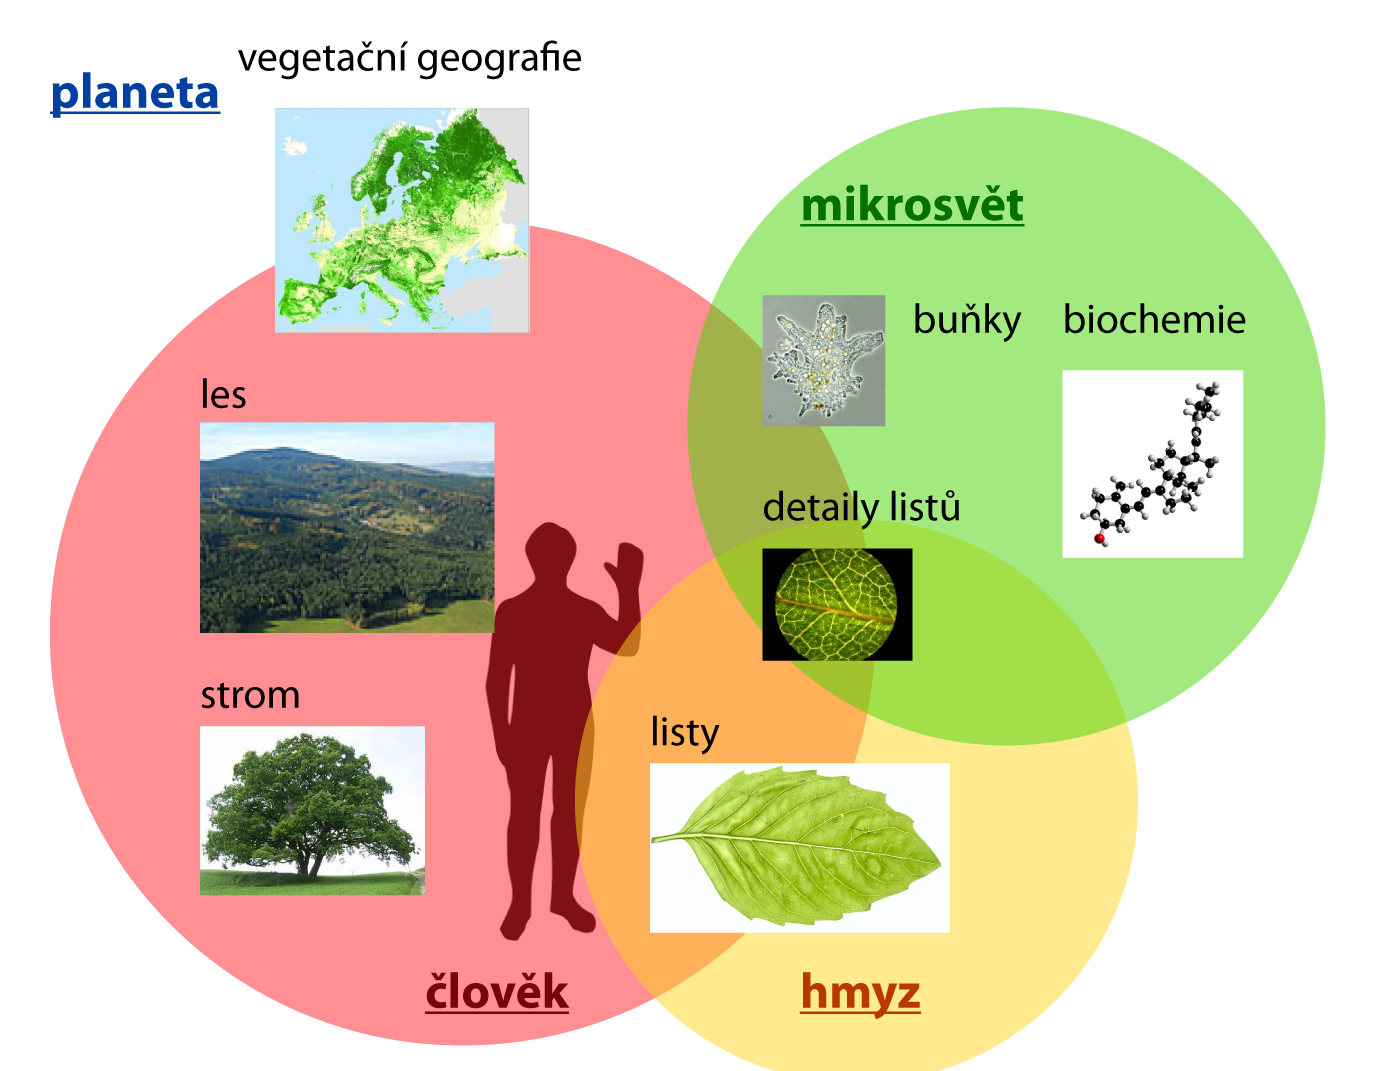
\includegraphics[width=0.7\textwidth]{./figures/DETAIL.png}

\caption{Znázornění příkladu úrovní detailu. }
\label{fig:Levels_of_detail}
\end{center}
\end{figure}

Pokud budeme na chvíli chápat úroveň detailu tímto způsobem, uveďme, že tato práce se pohybuje výhradně na úrovni pohledu člověka, neboť právě virtuální simulace pohledu člověka na vegetaci je jejím předmětem.
Samozřejmě je možné navrhnout i jiné systémy, které zpřístupní uživatelům informace na ostatních úrovních detailu, ale to je již úloha z oboru vizualizace a řada postupů by byla zřejmě zcela odlišná.
Souvislost tohoto přirozeného systému úrovní detailu s již zmíněným technickým pojetím ale existuje. Jak bude popsáno dále, v současné době není v možnostech běžného hardwaru zobrazovat jednotným postupem lesy o tisícovkách stromů i detail jednotlivých listů samostatného stromu dostatečnou rychlostí pro real-time aplikace. Přirozený systém úrovní detailu rovněž napovídá, jak uživatel vnímá určité pohledy. Při pohledu na celý rozsáhlý les stromů jsou tím nejpodrobnějším, co uživatel rozpozná, jednotlivé stromy, případně nejvýraznější větve, největší pozornost je zaměřena na celkový tvar lesa, tvar čáry horizontu, hustotu a druhovou skladbu jednotlivých rostlin. Pohled na úrovni jednotlivého stromu naproti tomu musí zobrazit i jednotlivé větve a listy, tvar lesa již není tak důležitou informací. Pokud přejdeme ještě blíž, uživatel by měl mít možnost pozorovat i detaily na listech. Z toho může vycházet technická stránka úrovně detailu (dále jen LOD).

Cílem této práce je navrhnout a poté realizovat software, který bude realisticky zobrazovat stromovou vegetaci v reálném čase a umožní i její animaci (působením větru). Software by měl pracovat na běžně dostupném hardware. Dále bude software poskytovat podporu pro zobrazování stromů v různých obdobích roku. Půjde především o změnu barvy listí. Práce se bude pohybovat na úrovni podrobnosti běžné pro vnímání člověka. Tedy umožní zobrazit větší skupinu stromů (les) a přitom bude možné pozorovat jednotlivé listy stromů a to včetně animace. Práce se zaměří především na způsob, jakým lze stromy na těchto úrovních podrobnosti zobrazovat v pohybu.

%%%%%%%%%%%%%%%%%%%%%%%%%%%%%%%%%%%%%%%%%%%%%%%%%%%%%%%%%%%%%%%%%%%%
\section{Stávající řešení}

Zobrazování vegetace v reálném čase je vcelku běžný požadavek současných grafických systémů - především herních enginů. Jak ukazuje například článek \cite{Mantler_2003_SARRV}, existuje množství různých přístupů. Mohou být veskrze rozděleny podle toho, zda pracují přímo s prostorovou geometrií modelu (3D reprezentace), či s dvourozměrnou náhražkou (2D reprezentace). Každý přístup má svá pro i proti a existuje i mnoho způsobů, jak je kombinovat.
 
\subsection{Trojrozměrná geometrická reprezentace}
Základní verze 3D povrchové reprezentace modelu vychází z myšlenky, že pokud je těleso neprůhledné (neprůsvitné), stačí k jeho zobrazení vykreslit jen jeho povrch. Povrch tělesa je popsán množinou trojúhelníků v prostoru a jejich barvou (texturou) - případně dalšími atributy. Trojúhelník reprezentuje část geometrie skutečného modelu. Avšak je nutné si uvědomit, že možnosti současných grafických karet jsou omezené a jejich výkon pro real-time (zhruba 25 fps) se pohybuje pouze v řádech desítek milionů zpracovaných trojúhelníků  (při základní pipeline). Tato hranice se ještě výrazně sníží, pokud požadujeme pokročilejší zpracování (například složitější model osvětlení, více texturovacích zdrojů, atd.). Z výše uvedených omezujících faktorů vyplývá, že přímé zobrazení např. celého lesa na úrovni vykreslování trojúhelníků, coby geometrie reprezentující jednotlivé listy, je příliš náročné i pro současný hardware.
Zajímavé metody a přístupy, jak zobrazovat kvalitně a efektivně i detailní geometrii stromů včetně animace až na úrovni jednotlivých listů jsou popsány v článcích \cite{Habel_09_PGT} a \cite{Habel_2007_RTT}. 
\begin{figure}[here]
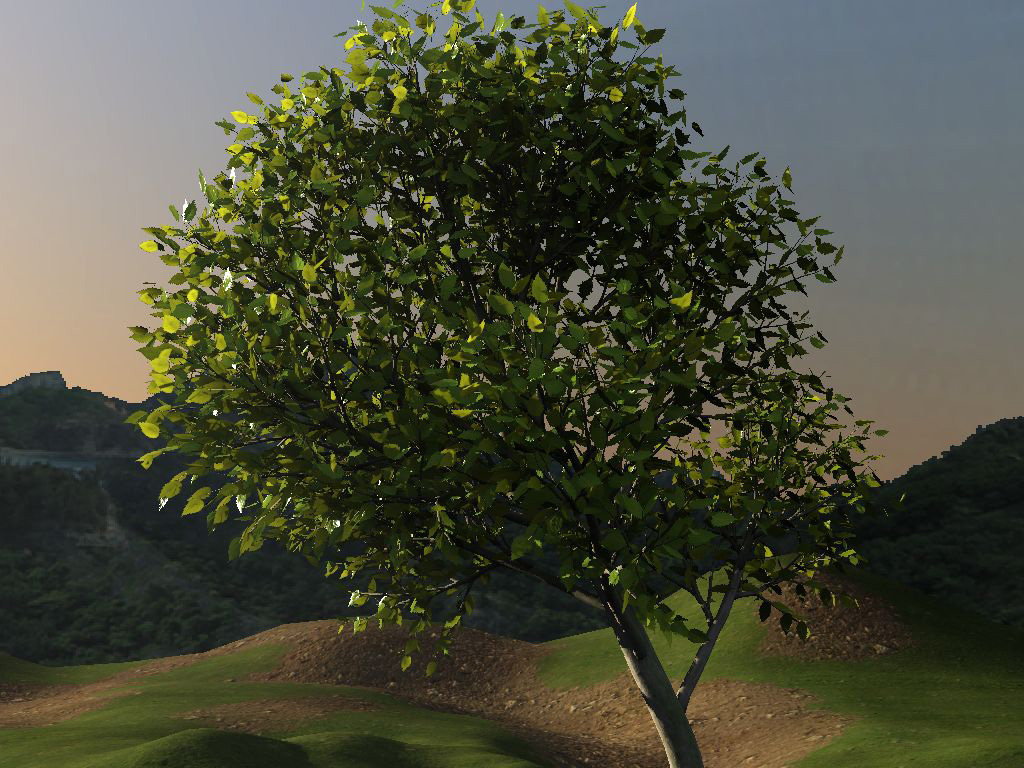
\includegraphics[width=0.5\textwidth]{./figures/HABEL_tree.jpg}
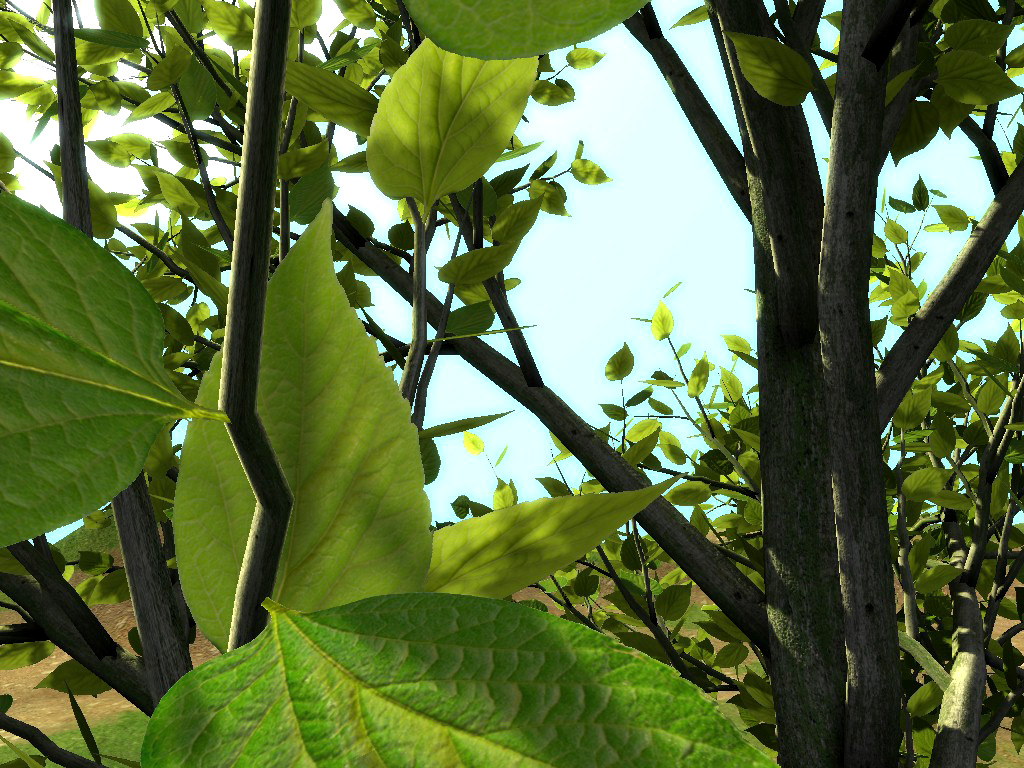
\includegraphics[width=0.5\textwidth]{./figures/HABEL_leaves.jpg}
\caption[Možnosti realistického zobrazování vegetace]%
{Možnosti realistického zobrazování vegetace, převzato z \cite{Habel_2007_RTT} }
\label{fig:HABEL_leaves}
\end{figure}
Jsou navrženy postupy, které berou v potaz rozdílné vlastnosti různých stran listů i jejich průsvitnost. Animace stromu je optimalizována pro zpracování na GPU ve vertex shaderu a pracuje na principu hierarchické deformace geometrie na úrovni jednotlivých hierarchických úrovní větví. Avšak zobrazení většího počtu stromů je i tak příliš náročné na výkon a není zde řešeno.

Existuje však i možnost, jak zobrazení optimalizovat. K tomu účelu se hojně využívá technik zjednodušování geometrie 3D objektu. Složitost geometrie přechází ve složitost materiálu. Pokud zůstaneme u tématu vegetace, pak si lze představit, že původní 3D reprezentace např. stromu obsahuje geometrický popis i nejmenších detailů křivosti jednotlivých listů. V tom případě by stačila jen informace o barvě geometrických primitiv a výsledný obrázek po vykreslení by mohl být velmi kvalitní. Učiňme myšlenkový krok zjednodušení geometrie tak, že jednotlivý list reprezentuje pouze jeden trojúhelník. Křivost samotného listu pak musí obsáhnout složitější informace o materiálu listu. Pokud bychom reprezentovali např. celou větev se všemi listy jedním trojúhelníkem, složitost materiálu musí zákonitě narůst příslušným způsobem, pokud požadujeme alespoň přibližně stejný výsledek zobrazení.

\begin{figure}[!htb]
\begin{center}
$\begin{array}{ccc}
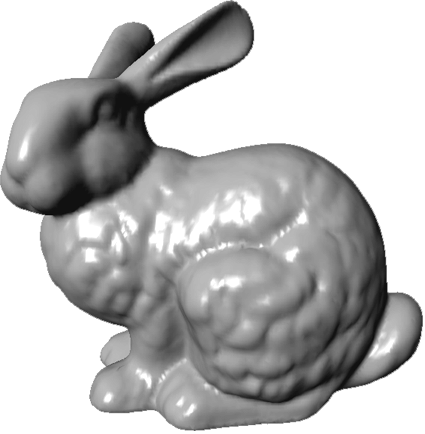
\includegraphics[width=0.2\textwidth]{./figures/bunny_lod_0.png}&

\includegraphics[width=0.2\textwidth]{./figures/bunny_lod_3.png}&
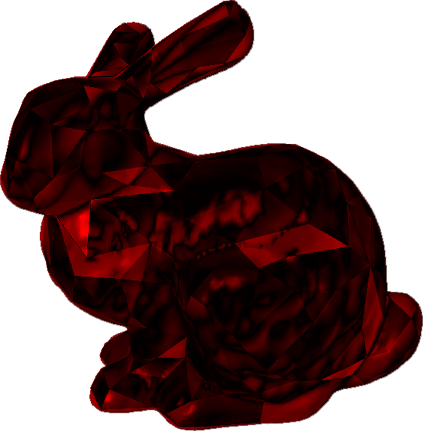
\includegraphics[width=0.2\textwidth]{./figures/bunny_lod_diff.png}
\\
(a)&(b)&(c)
\end{array}$
\end{center}
\caption[Obrazy různých stupňů detailu téhož modelu]%
{Obrazy různých stupňů detailu téhož modelu $(a)$ a $(b)$ a jejich rozdíl červeně $(c)$}
\label{fig:BUNNY_lod}
\end{figure}
Pokud metoda zobrazování a řízení úrovně detailu nepracuje dynamicky (což většinou zajišťuje takřka nepostřehnutelný přechod mezi úrovněmi), vyvstává vždy problém, jak provádět přechod mezi jednotlivými úrovněmi, který při naivním přepnutí úrovní může vést k nevítanému efektu zvanému \emph{LOD-popping}. Jde o to, že pokud se skokově změní velká část obrazu, vnímá tuto změnu pozorovatel velmi rušivě.
Klasická metoda snížení LOD-poppingu pracuje s prolínáním obrazů a řízením jejich průhlednosti. Zatímco jedna úroveň je postupně zprůhledňována a mizí, druhá se naopak stává neprůhlednou a objevuje se. Během tohoto přechodu se ovšem může stát, že se model stane průhledným, jak ukazuje obrázek  ~\ref{fig:BUNNY_lod_trans}.
\begin{figure}[!htb]
\begin{center}
$\begin{array}{ccc}
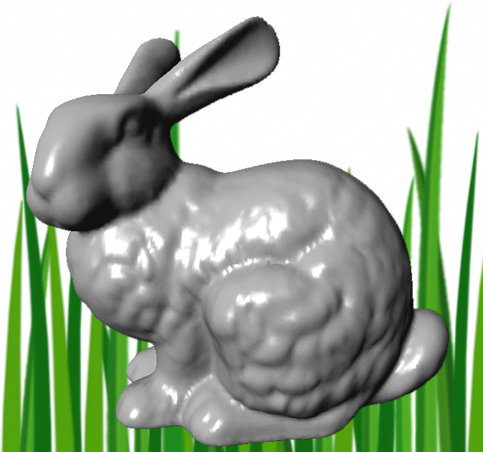
\includegraphics[width=0.2\textwidth]{./figures/bunny_lod_trans_01.png}&
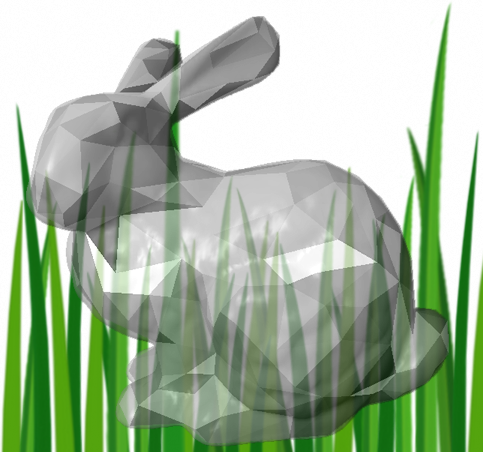
\includegraphics[width=0.2\textwidth]{./figures/bunny_lod_trans_02.png}&
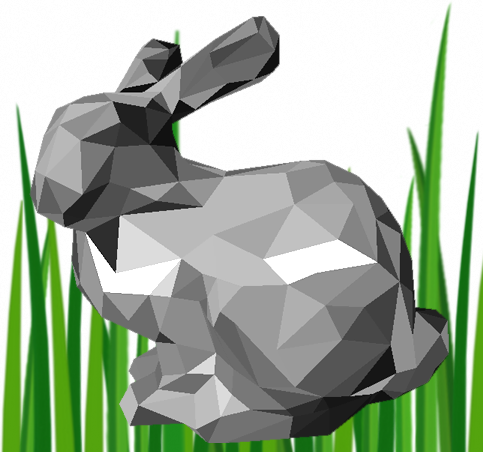
\includegraphics[width=0.2\textwidth]{./figures/bunny_lod_trans_03.png}
\\
(a)&(b)&(c)
\end{array}$
\end{center}
\caption[Znázornění problémů měkkého přechodu mezi diskrétními úrovněmi detailu]%
{Znázornění problémů měkkého přechodu mezi diskrétními úrovněmi detailu.
\newline
$(a)$ LOD0 100\% , LOD1 0\% \newline
$(b)$ LOD0 50\% , LOD1 50\%, objekt se stal průhledným, ačkoliv by neměl. \newline
$(c)$ LOD0 0\% , LOD1 100\% 
\label{fig:BUNNY_lod_trans}
}
\end{figure}
Eliminací tohoto nežádoucího efektu se zabývá článek \cite{GIEGL-2007-UNP}. Jde o postup, kdy je vždy jedna úroveň detailu zobrazena plně a neprůhledně. Tím je zaručeno, že nemůže dojít k celkovému zprůhlednění. 
%%%%%%%%%%%%%%%%%%%%%%%%%%%%%%%%%%%%%%%%%%%%%%%%%%%%%%%%%%
\pagebreak
\subsection{Reprezentace založené na obrázcích}

%\begin{figure}[here]
%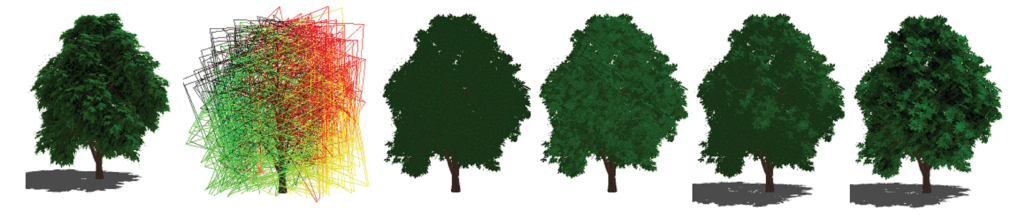
\includegraphics[width=1.0\textwidth]{./figures/garcia_billboardclouds.png}
%\caption{Reprezentace korum stromů pomocí billboadcloudů, převzato z \cite{GIPGSMSL07_images} }
%\label{fig:GARCIA_billboardcloud}
%\end{figure}


Způsob, jak optimalizovat proces zobrazování pomocí seskupení podobně orientovaných listů z celé koruny stromu do billboardů je popsán v článku \cite{GIPGSMSL07}. Vegetace je pak reprezentována tzv. billboardcloudem. Bohužel, ačkoliv je tento přístup velmi slibný pro statické modely, pokud požadujeme věrohodnou animaci vegetace, pak nelze předpokládat, že všechny obdobně orientované listy na různých větvích se budou chovat stejným způsobem.
\begin{figure}[here]
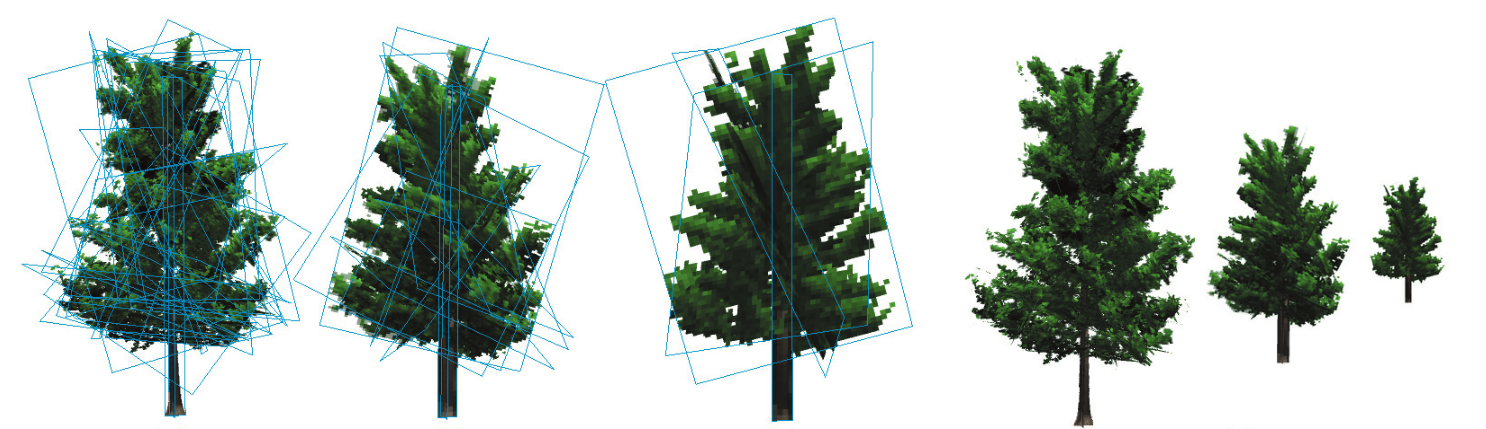
\includegraphics[width=1.0\textwidth]{./figures/umlauf_lod.png}
\caption[Různé úrovně detailu tvořené billboardy a jejich porovnání]%
{Různé úrovně detailu tvořené billboardy a jejich porovnání při použití (zcela vpravo), převzato z \cite{Umlauf05} }
\label{fig:UMLAUF_lod}
\end{figure}
Myšlenka seskupení blízkých listů za účelem zjednodušení geometrické složitosti modelu je vyjádřena v článku \cite{Rebollo_07_FRL}, kde jsou listy dynamicky slučovány na základě jejich prostorové blízkosti a podobnosti. Ačkoliv jsou navrhované postupy daleko vhodnější pro přidání možnosti animace, jde v zásadě o dynamické řízení úrovně detailu a jako takové vyžadují relativně výrazné prostředky pro správu zjednodušovaného modelu. 

Existuje i několik přístupů založených čistě na billboardingu. Metoda řezů představená v článku \cite{Jakulin00} vytváří určitý trs billboardů, které zobrazují pohledy z několika směrů a to i v několika vrstvách (viz obr. ~\ref{fig:JAKULIN_slices}).
\begin{figure}[!htb]
\begin{center}
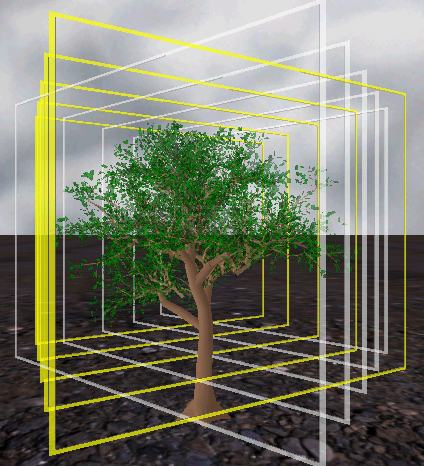
\includegraphics[width=0.3\textwidth]{./figures/slicingJakulin.jpg}
\end{center}
\caption[Reprezentace korum stromů pomocí řezů]%
{Reprezentace korum stromů pomocí řezů, převzato z \cite{Jakulin00} }
\label{fig:JAKULIN_slices}
\end{figure}
 Trs billboardů je v tomto případě vůči scéně nehybný a řezy, které jsou souběžné se směrem pohledu, jsou skrývány. Výhoda použití více souběžných billboardů spočívá v tom, že lze tímto způsobem navodit dojem určité prostorové hloubky (efekt paralaxy).

Metoda trsu rovnoběžných billboardů je rozpracována i v článku \cite{Truelsen_08}, kde je popsána možnost, jak efektivně řídit úrovně detailu pro tyto trsy.

Dovedeme-li zjednodušení do takové krajnosti, že původní objekt (či dokonce skupiny objektů) reprezentujeme jedním geometrickým primitivem, mluvíme o takzvaných billboardech, či impostorech (viz obr. ~\ref{fig:UMLAUF_billboards}). 
Díky vlastnostem lidského vnímání a zobrazovací technoliogii je možné nahradit určitý objekt plochým obrazem, který odpovídá pohledu na daný objekt z podobného místa. 
\begin{figure}[!htb]
\begin{center}$
\begin{array}{cc}
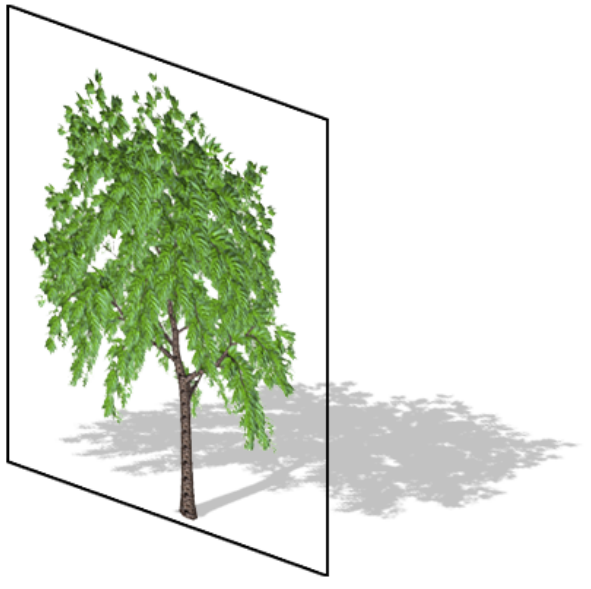
\includegraphics[width=0.25\textwidth]{./figures/billboard_a.png}&
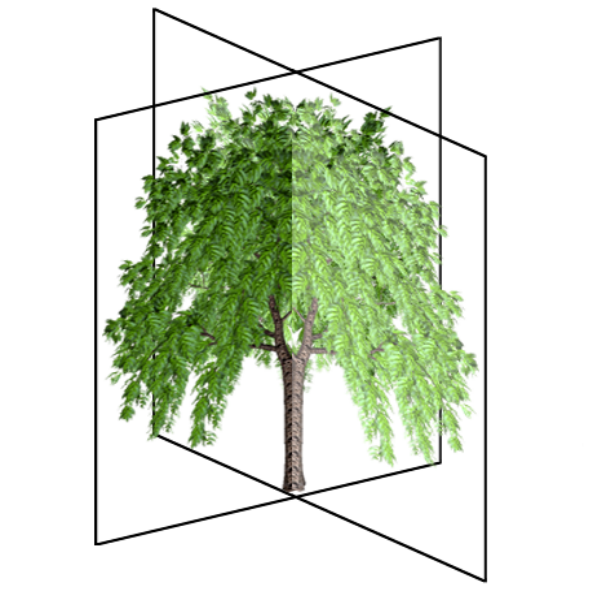
\includegraphics[width=0.25\textwidth]{./figures/billboard_b.png}\\
(a)&(b)
\end{array}$
\end{center}
\caption[Různé přístupy k billboardům]%
{Různé přístupy k billboardům. Jediný plochý obraz, který se natáčí k pozorovateli $(a)$ , křížová konstrukce dvou billboardů, které zachovávají orientaci vůči scéně $(b)$, převzato z \cite{Umplauf_MT} }
\label{fig:UMLAUF_billboards}
\end{figure}
Zatímco zpracování geometrických primitiv je relativně pomalý proces, uplatnění informací o materiálu v daném bodě může být velmi efektivní. Nutno ovšem dodat, že běžné reprezentace materiálu (obrázkové textury) trpí omezeními plynoucími z jejich principu – např. omezené rozlišení. Tedy jakési plnohodnotné nahrazení původní 3D geometrie funguje obstojně jen pro objekty ležící za určitou rozlišovací hranicí, která je dána zejména faktory jako rozlišení textur, rozlišení obrazovky, detailnost pohledu, geometrická podobnost obou reprezentací a podobně. 



%%%%%%%%%%%%%%%%%%%%%%%%%%%%%%%%%%%%%%%%%%%%%%%%%%%%%%%%%%
\subsection{Volumetrické zobrazování a bodové mraky}
Existují však ještě další možnosti, jak reprezentovat a zobrazovat vegetaci. Metoda vycházející z principů volumetrického zobrazování (volume rendering) je popsána v článku \cite{DN04}. Je vhodná zejména pro úroveň detailu typu les a vegetační geografie. Nicméně její přímé využití pro zobrazování na úrovni jednotlivých listů je s dnešním běžným hardware nemožné. Metoda pracuje s rovnoběžnými vrstvami textur, jejichž hustota je řízena aktuální úrovní detailu v daném místě.
\begin{figure}[here]
\begin{center}
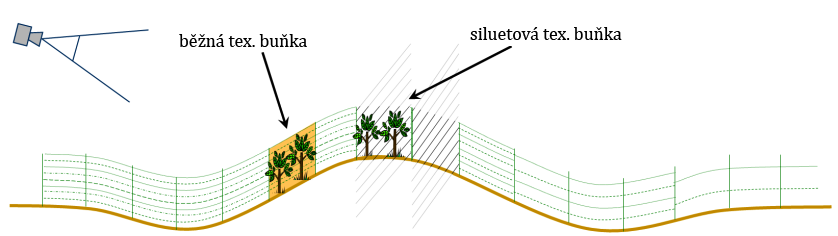
\includegraphics[width=1.0\textwidth]{./figures/a1_slicing.png}
\end{center}
\caption[Volumetrické zobrazování využívající rovnoběžných textur]%
{Volumetrické zobrazování využívající rovnoběžných textur, převzato z \cite{DN04}
}
\label{fig:VOLUME_texcells}
\end{figure}

Další možností je tzv. bodové (nebo-li \emph{point-based}) zobrazování. Základním primitivem tohoto přístupu je prostorový bod (dále jen bod). Tato metoda je výhodná zejména pro objekty, které jsou promítnuty do malého počtu pixelů na výstupním zařízení, neboť pro jejich věrné zobrazení stačí minimálně tolik bodů, kolik pixelů na zobrazovacím zařízení zabírají. Ovšem neplatí zde, že prostorový bod je vždy promítnut do právě jednoho pixelu. Velikost a tvar, jímž je reprezentován bod, se mohou lišit. Nabízí se tedy, aby list stromu byl reprezentován právě jedním bodem. Ovšem i tehdy by byl počet zpracovávaných bodů příliš veliký při zobrazování celého lesa naivním postupem. Pokročilé techniky LOD jsou navrženy v článku \cite{GMN05}. Prostor je rozdělen do pravidelné mřížky a v rámci vzniklých buněk je určen LOD. Na nejvyšší úrovni LOD reprezentuje skutečně každý bod specifický list, ovšem s nižší úrovní LOD jsou listy slučovány a postupně reprezentovány většími body (viz obr. ~\ref{fig:PB}) . 
\begin{figure}[!hbt]
\begin{center}
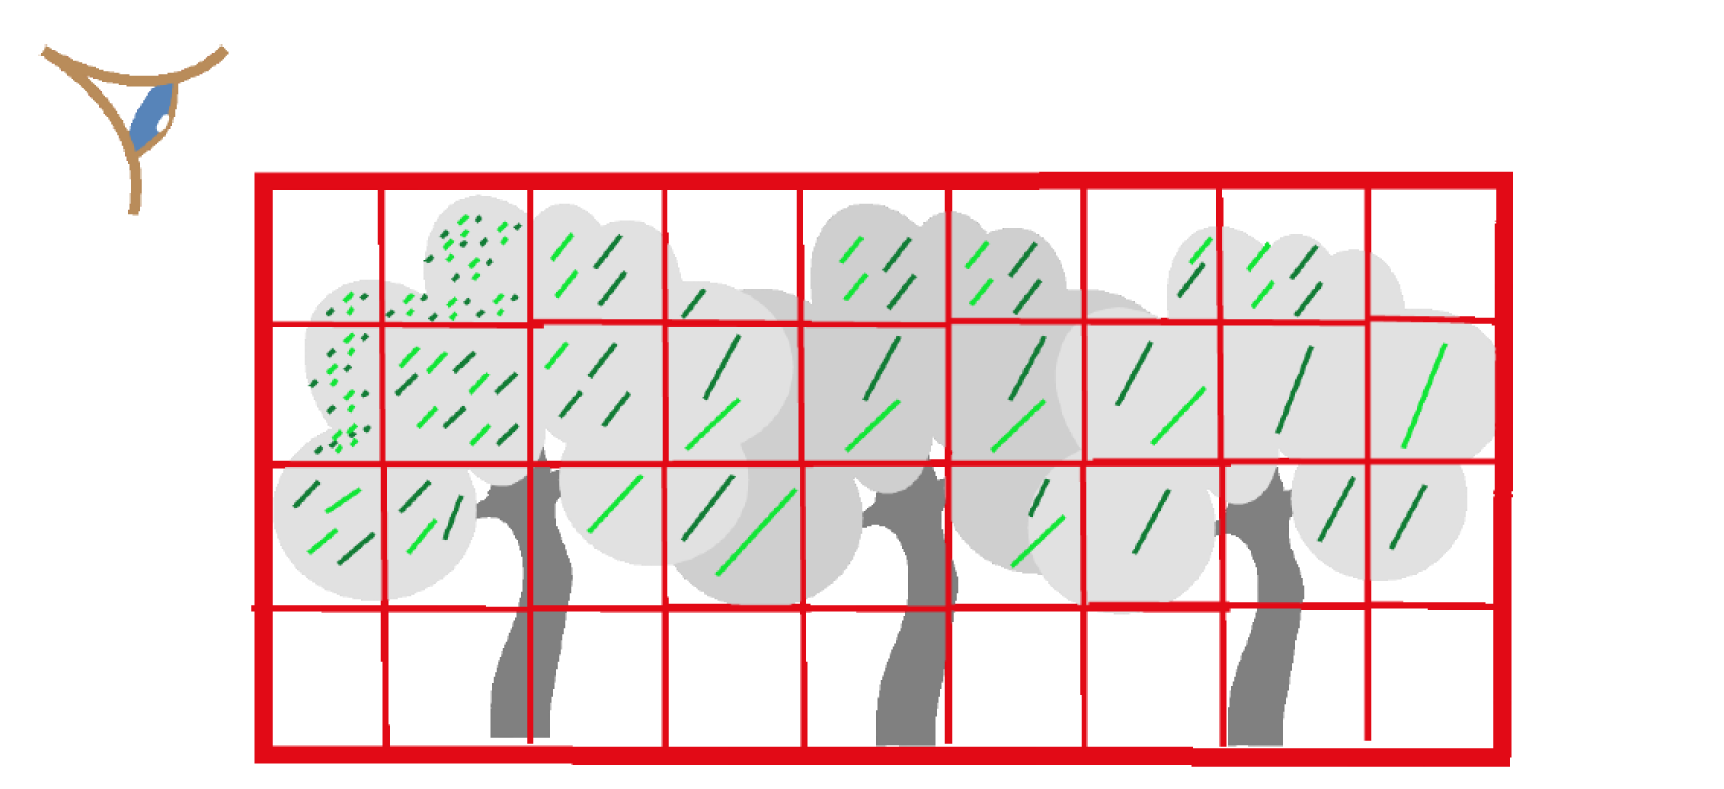
\includegraphics[width=1.0\textwidth]{./figures/point-based.png}
\end{center}
\caption[Reprezentace listů jednotlivými body]%
{Reprezentace listů jednotlivými body. Čím je zobrazovaný bod dále od kamery, tím je větší a reprezentuje více listů. Převzato z \cite{GMN05}
}
\label{fig:PB}
\end{figure}
 
Vzdálenější koruny stromů jsou tak reprezentovány malým počtem velkých bodových primitiv, protože platí předpoklad, že tyto primitiva se zobrazí do jednoho (maximálně několika málo) výsledných pixelů. Bodová reprezentace v tomto podání funguje velmi dobře jen pro korunu stromu. Použití i pro samotný kmen a větve stromu je problematické. 
%%%%%%%%%%%%%%%%%%%%%%%%%%%%%%%%%%%%%%%%%%%%%%%%%%%%%%%%%%
\pagebreak
\subsection{Zhodnocení stávajících řešení}
Jak se ukazuje, všechna řešení pracující až na úrovni jednotlivých listů pracují s geometrickým trojrozměrným modelem stromu (povrchová trojúhelníková reprezentace). Každá z metod zobrazující současně strom na úrovni listů i rozsáhlý les využívá nějakou formu řízení úrovně detailu. Tím dosahují snížení složitosti scény a vyšší efektivity. Zatímco metod zaměřujících se pouze na statické zobrazení je celá řada, postupů, jak jednotlivé stromy realisticky rozhýbat je málo a omezují se na geometrické modely. Některé techniky LOD by bylo obtížné přizpůsobit, aby efektivně fungovaly i pro pohybující se stromy (volumetrické reprezentace). Jiné by bylo možné s relativně rozumným úsilím rozšířit i o tuto možnost (billboard-clouds). Metody dynamického řízení úrovně detailu většinou představují elegantní řešení, které netrpí problémy LOD-poppingu, ale vyžaduje zvýšené prostředky na neustálé udržování aktuální úrovně detailu modelů. Naproti tomu diskrétní LOD systémy se musí vypořádávat s přepínáním jednotlivých úrovní, ale představují jen malou výkonostní zátěž. Ať už dynamické či diskrétní LOD systémy, nejčastěji se využívá převedení složitosti geometrie do obrazu, který je pak namapován na zjednodušenou geometrii.



%*Analýza a návrh řešení****************************************************************************
\chapter{Analýza a návrh řešení}
\label{chap:analyza}

Pro účely real-time renderování grafiky se běžně využívá metod přímé rasterizace\footnote{V současnosti existují i přístupy využívající technik sledování paprsku (ray tracing) pracující v real-time. Pro některé scény mohou být dokonce efektivnější, nicméně jejich implementace na GPU je obtížnější a standardem v oboru real-time počítačové grafiky je stále přímá rasterizace.}. Existuje několik grafických API, které pro tyto účely využívají grafický hardware a dosahují tak pozoruhodného výkonu. Dvěmi nejběžnějšími API pro práci s 3D grafikou jsou v současnosti DirectX a OpenGL. Technologie DirectX je standardem v oblasti počítačových her a je vázaná na platformu Windows. Naproti tomu OpenGL je platformově nezávislá knihovna dosahující srovnatelných výsledků. Obě technologie pak pracují s GPU a využívají tzv. grafickou pipeline poskytovanou hardwarem.
Z průzkumu stávajících řešení vyplývá, že realistického real-time zobrazení na úrovni listů lze v současné době dosáhnout efektivně využitím geometrické ploškové reprezentace. Pro její zpracování je optimalizován grafický hardware a takto popsané stromy lze i věrně rozpohybovat. Jeví se proto jako výhodné, využít ji pro zobrazování instancí stromů s nejvyšším stupňěm detailu. Postup zpracování grafických primitiv na GPU je znázorněn na obrázku (~\ref{fig:gpupipeline}).

\begin{figure}[!hbt]
\begin{center}
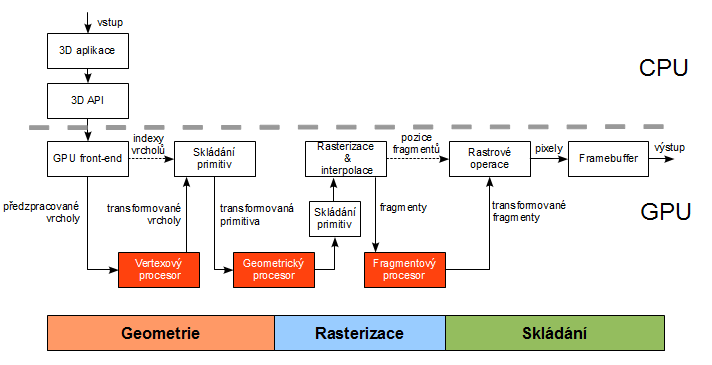
\includegraphics[width=0.85\textwidth]{./figures/GPUpipeline.png}
\end{center}
\caption[Grafická pipeline]%
{Grafická pipeline. Oranžově zvýrazněné bloky lze přeprogramovat a využít k vlastnímu zpracování grafiky.
\label{fig:gpupipeline}
}
\end{figure}

Nížší úrovně následně vytvořeného LOD-systému budou z této nejpodrobnější úrovně odvozeny a abstrahovány. Pro věrné zobrazení stromu pohybujícího se vlivem větru je třeba poznat, jak na vítr strom reaguje. Teoretické základy takové animace rozebere právě následující sekce.

%%%%%%%%%%%%%%%%%%%%%%%%%%%%%%%%%%%%%%%%%%%%%%%%%%%%%%%%%%%
\section{Animace geometrického 3D modelu}
\label{sec-animation3D}

Jelikož je model tvořen množinou trojúhelníků a ty mají přímou vazbu na části stromu (list, konkrétní větev), lze tedy vhodnou změnou jejich polohy animovat celý strom. Požadavek na provádění animace v reálném čase prakticky implikuje i potřebu využití GPU pro tyto účely. Grafická primitiva tvořící model jsou zpracovávána na GPU po vrcholech (vertexech) ve vertex shaderu, který může měnit jejich pozici. 
Metoda, jíž lze s výhodou použít, je popsaná v již zmíněném článku \cite{Habel_09_PGT} a využívá myšlenky tzv. hierarchical vertex displacement. Důležitý je zde fakt, že skutečné větve stromů tvoří hierarchickou strukturu a transformaci nadřazené větve v bodě napojení přejímá celá skupina větví podřízených, což tvoří netriviální řetěz transformací. Tato skutečnost svazuje do určité míry výpočet polohy nadřazené a z ní vycházející větve. Poskytneme-li však vhodná data každému vrcholu, může být celý řetěz transformací určen právě pro každý jednotlivý vrchol korektně a výpočet animace se tak provádí na GPU ve vetrex shaderu.

%%%%%%%%%%%%%%%%%%%%%%%%%%%%%%%%%%%%%%%%%%%%%%%%%%%%%%%%%%%%%
\subsection{Deformace větví}
\label{sec-branchDeformation}

Deformace tak složitých objektů, jako jsou stromy, vlivem větru je komplexní fyzikální problém. Na jeho složitosti mají zásadní vliv zejména dva faktory – netriviální mechanické vazby jednotlivých větví a turbulentní proudění vzduchu, které způsobuje výsledný pohyb. Oba faktory se navíc vzájemně ovlivňují. Aktuální pozice dané větve ovlivňuje proudění v okolí a opačně. I pokud bychom nahradili turbulentní proudění laminárním, jde o složitý problém. Samotný ohyb jedné větve lze sice relativně dobře popsat, ovšem musíme uvažovat, že každá větev je napojena na další a tím ovlivňuje její ohyb. Síly působící na listy i větve samotné vlivem proudění vzduchu se přenáší hierarchií větví až ke kmeni. Jde vlastně o složitý problém inverzní kinematiky, který pro takto složité struktury zatím nelze běžně řešit v real-time. 
\begin{figure}[!hbt]
\begin{center}
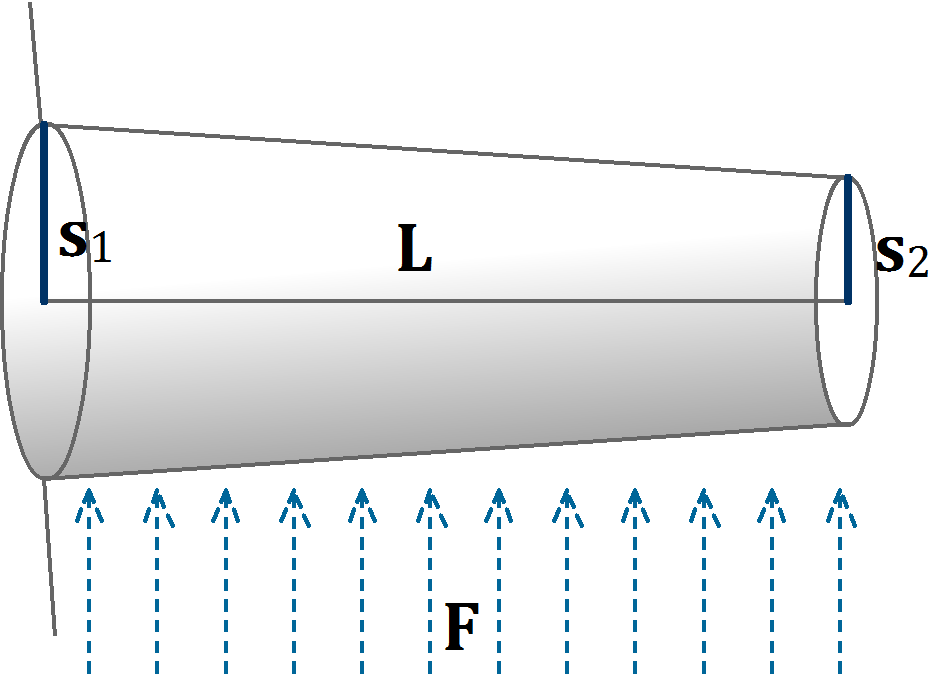
\includegraphics[width=0.25\textwidth]{./figures/branchBeamModel.png}
\end{center}
\caption{Fyzikální model pružného prutu (větve).
\label{fig:branchBeamModel}
}
\end{figure}

Aby bylo možné dosáhnout dostatečného zobrazovacího výkonu, je nutné rezignovat na úplnou fyzikální korektnost výpočtů deformace. Tuto relaxaci problému si naštěstí můžeme dovolit, neboť systém nemá ambice být fyzikálním simulátorem a předpokládá se, že uživatel se spokojí s výsledkem, který nebude výrazně porušovat jeho představu o deformaci vegetace.
Aby byla animace pohybu větví co nejvěrnější, je využita deformace vycházející z Euler-Bernoulliho popisu ohybu prutu. Větev je aproximována komolým kuželem s definovanou délkou $L$ a poloměry na počátku $s_1$ a na konci $s_2$. Tuhost tělesa je závislá pouze na průřezu. A na těleso působí kolmo síla $\vec{F}$ (viz obr. ~\ref{fig:branchBeamModel} ).

Euler-Bernoulliho rovnice pak popisuje ohyb takového tělesa:

\begin{equation}
\frac{\mathrm{d}^2 }{\mathrm{d} x^2}(EI(x)\frac{\mathrm{d}^2 \dot{u} (x))}{\mathrm{d} x^2} ) = F
\end{equation}

V tomto vztahu představuje $I$ plošný moment setrvačnosti a $E$ je modul pružnosti, který je uvažován jako konstantní. Okrajové podmínky na počátku (pevný konec) jsou :

\begin{equation}
\begin{array}{cc}
\dot{u} \mid _{x=0} = 0 & \frac{\mathrm{d} \dot{u} }{\mathrm{d} x}\mid _{x=0} = 0 \\
\end{array}
\end{equation}

a na konci jsou:

\begin{equation}
\begin{array}{cc}
\frac{\mathrm{d}^2 \dot{u} }{\mathrm{d} x^2} \mid _{x=L} = 0 & \frac{\mathrm{d}^3 \dot{u} }{\mathrm{d} x^3}\mid _{x=L} = 0 \\
\end{array}
\end{equation}

Provedeme zjednodušení, kde normalizujeme rozměry délkou $L$ a zavedeme konstantu $\alpha$, která udává poměr velikosti poloměrů na začátku a na konci prutu, také poupravíme modul pružnosti $E$ :

\begin{equation}
\begin{array}{ccc}
r_{1,2} = \frac{s_{1,2}}{L} &\alpha = \frac{r_2}{r_1} & {E}'= EL\\
\end{array}
\end{equation}

Plošný moment setrvačnosti pro kruhový průřez poloměru $r$ je dán vztahem:
\begin{equation}
I = \frac{\pi r^4}{4}
\end{equation}

Protože uvažujeme, že poloměr prutu se mění lineárně v podélné ose prutu, plošný moment setrvačnosti $I$ se mění takto:
\begin{equation}
I(x) = \frac{\pi r_{1}^4((\alpha -1)x + 1)^4}{4}
\end{equation}

Euler-Bernoulliho rovnice pro zmíněné okrajové podmínky a měnící se plošný moment setrvačnosti $I(x)$ má netriviální řešení
\begin{multline}
\dot{u}(x)=\frac{{E}'F}{r_{1}^4}(x(\alpha-1)(6+x(\alpha-1)(2x(\alpha-1)(3+(\alpha-3)\alpha)+3(4+(\alpha-2)\alpha)))\\
 - 6 (1+x(\alpha-1))^2 \log (1+x(\alpha-1))) \cdot  (3\pi(1+x(\alpha-1))^2(\alpha-1)^4)^{-1}
\end{multline}

\pagebreak
Tento vztah je však příliš složitý pro efektivní a rychlé vyhodnocení. Důležitý je postřeh, že funkce $\dot{u}$ je lineárně závislá na velikosti síly $|\vec{F}|$. Fitováním nalezneme funkci s velmi podobným průběhem ve tvaru:

\begin{equation}
\label{eq:bendFunction}\mathbf{
u(x) = c_2 x^2 + c_4 x^4}
\end{equation}

Koeficienty $c_2$ a $c_4$ reprezentují hodnoty ${E}'$, $\alpha$ a $r_1$. Ohybová funkce $u(x)$ tedy určuje, jaká bude výchylka bodu kolmo na podélnou osu prutu ve vzdálenosti $x$ od počátku větve (předchozí normování zajišťuje, že větev zde má vždy jednotkovou délku). Vytváří tak ohybovou křivku. Derivaci ohybové funkce v bodě $x$ označíme ${u}'(x)$.

Ovšem bod na ohýbaném prutu se ve skutečnosti nepohybuje po přímce kolmé k podélné ose, nýbrž opisuje složitou křivku danou i faktem, že délka prutu se při deformaci nemění. Pokud by však byl použit přímo tento vztah pro deformaci, docházelo by k viditelnému efektu prodlužování prutu (větve) s většími výchylkami. Z toho důvodu je nutné zavést určitou korekci, jež bude ve výsledku zachovávat stejnou délku prutu pro libovolnou výchylku. Pokud bychom chtěli zachovat přesnou délku, bylo by nutné vždy vyřešit křivkový integrál, což je příliš časově náročné, a proto se spokojíme s nepřesnou, avšak dostačující a především rychlou metodou.
Vyjdeme z předpokladu, že pro korekci délky stačí posunout bod $P_0$ o určitou vzdálenost $d$ po přímce tečné v tomto bodě s ohybovou křivkou. Získáme tak výsledný bod $P$. 

\begin{figure}[!hbt]
\begin{center}
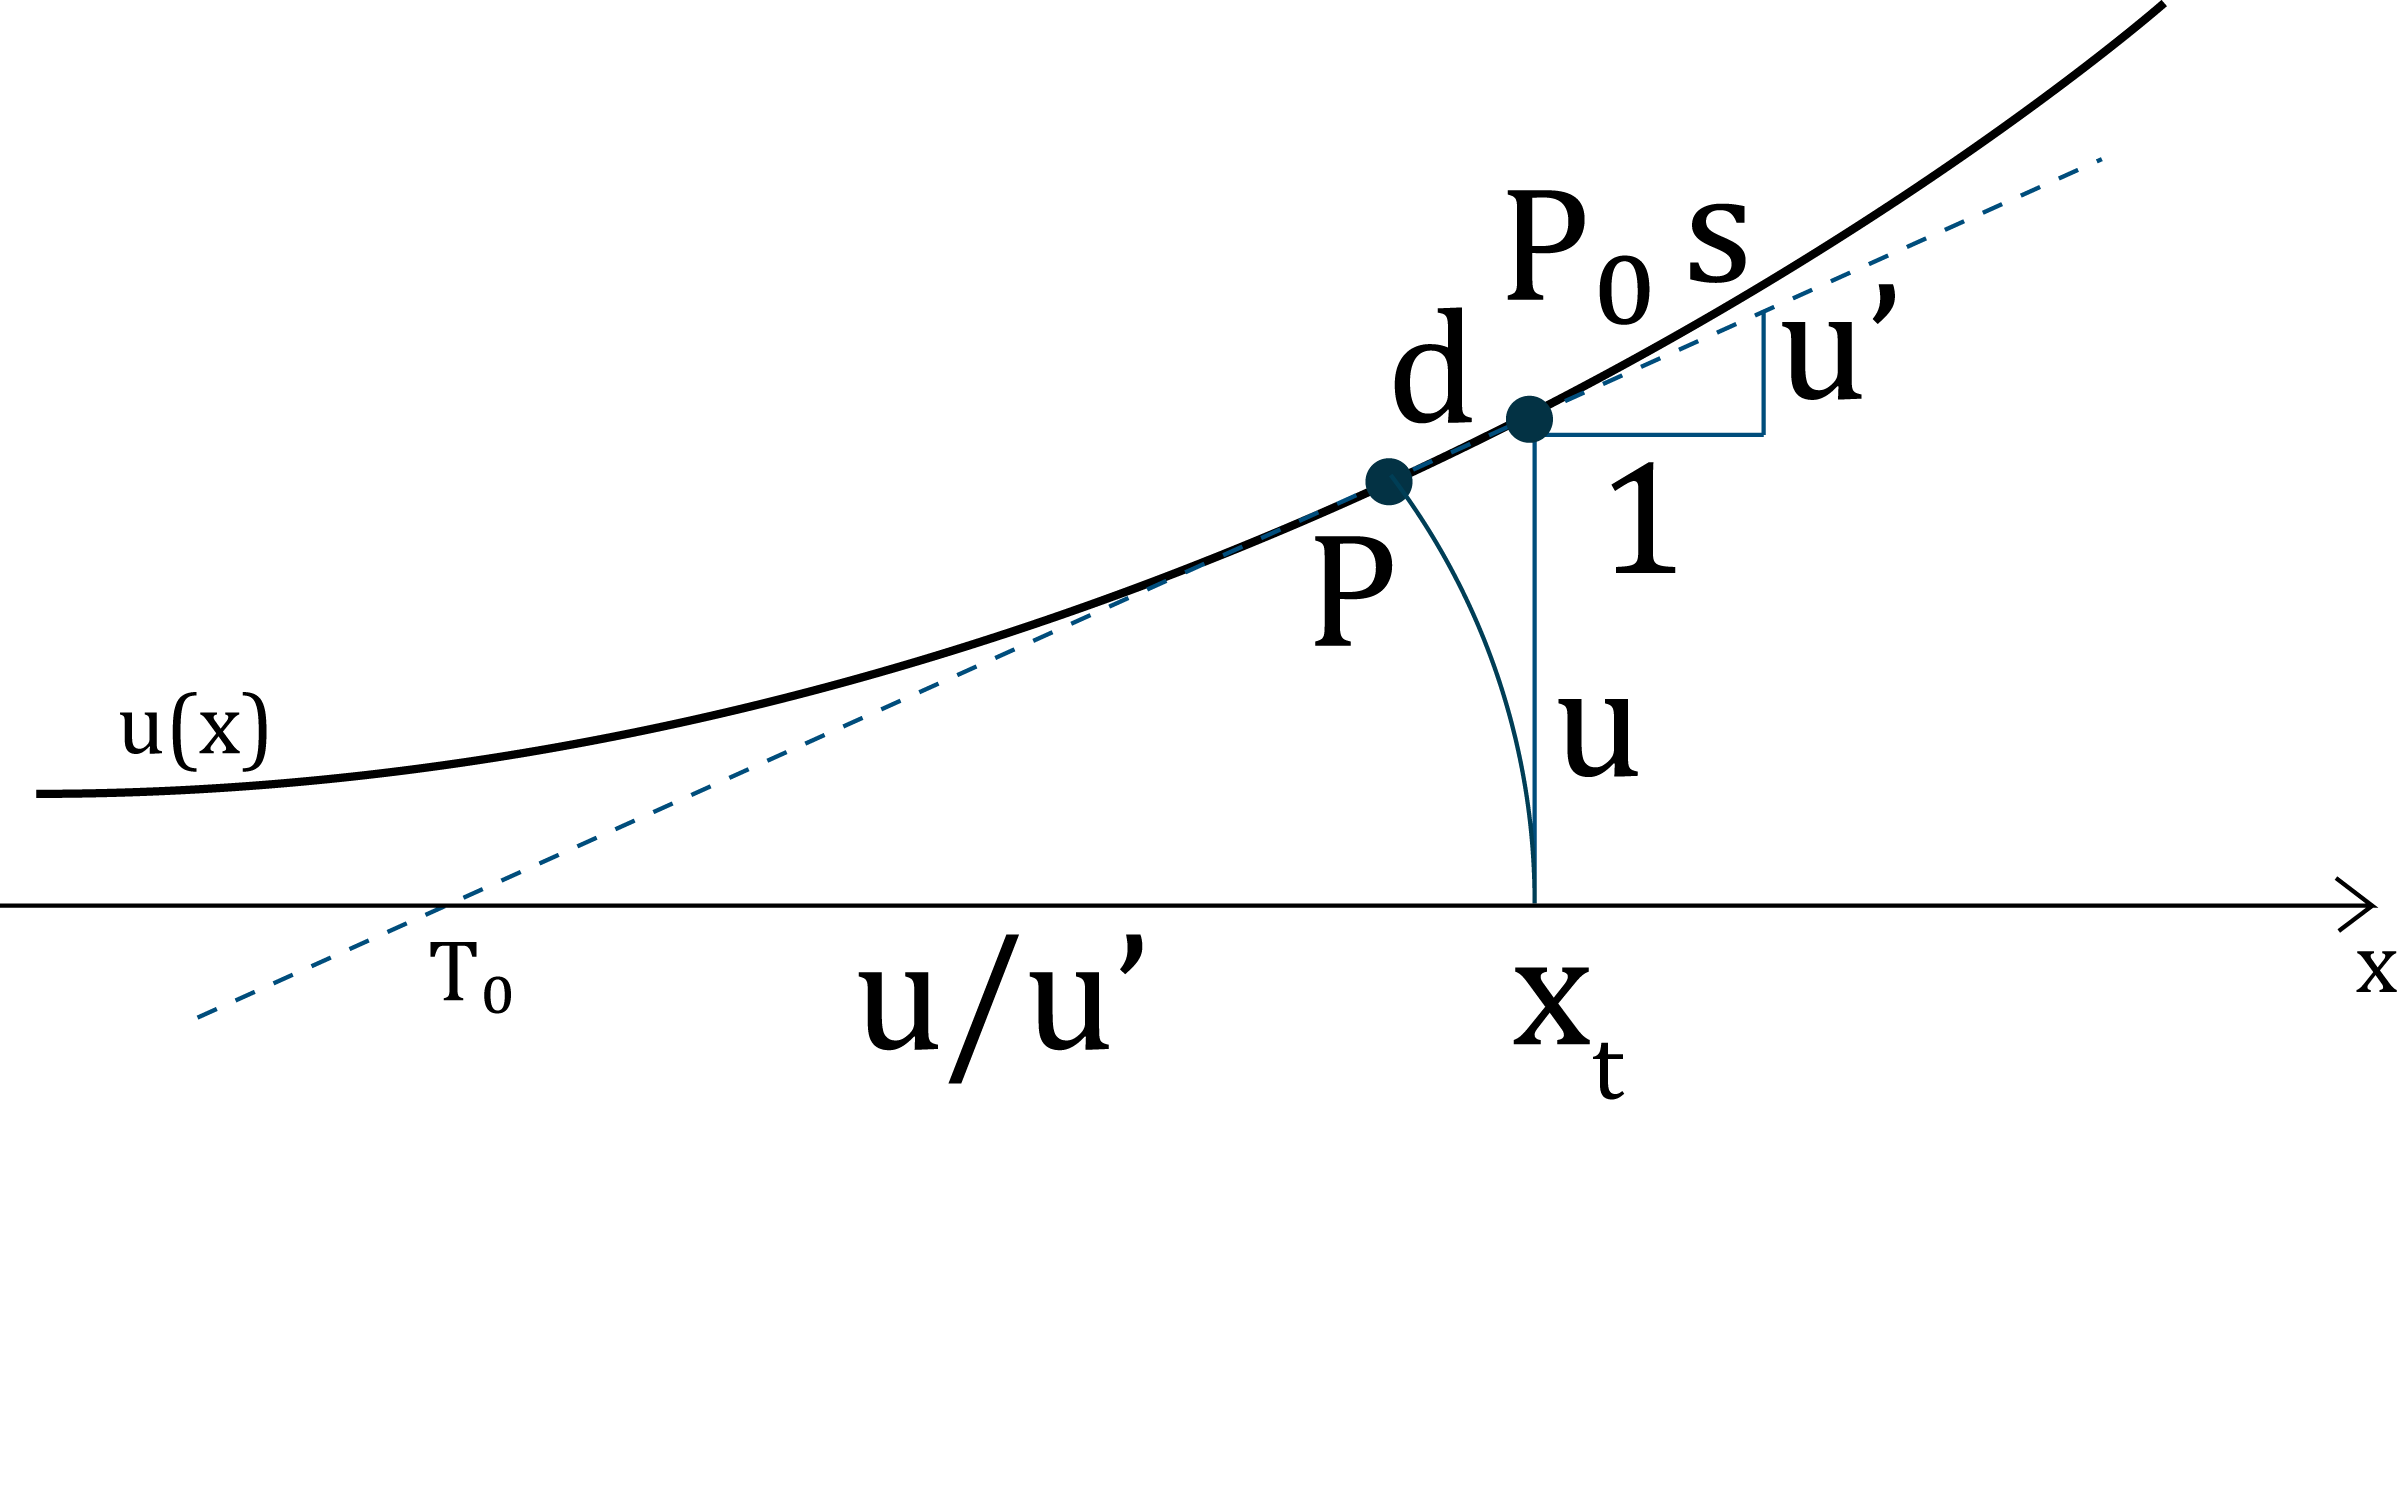
\includegraphics[width=0.5\textwidth]{./figures/lengthCorrection3.png}
\end{center}
\caption[Korekce délky ohybové funkce]%
{Korekce délky ohybové funkce $u(x)$. Pro přehlednost byl ze zápisu vypušten parametr $x_t$. Místo $u(x_t)$ je zapsáno pouze $u$ a obdobně pro další.
\label{fig:bendCorrection}
}
\end{figure}

Uvažujeme-li o deformaci jako o rotaci, pak na základě podobnosti trojúhelníků a zachování délek $|T_0x_t|$ a $|T_0P|$ můžeme zformulovat následující korekční vztahy (postup nazývejme „korekce délky“ ):

\begin{align} 
 \label{lengthCorrection}
s(x) &= \sqrt{1 + u'^{2}(x)}\nonumber\\
d(x) &= \frac{u(x)}{u'(x)}(s(x)-1)\nonumber
\\
\vec{p} &= \vec{p}_0 + \frac{1}{s(x)}\begin{pmatrix}
-d(x)\\u(x) 
\end{pmatrix}
\end{align}

 

\begin{figure}[!hbt]
\begin{center}
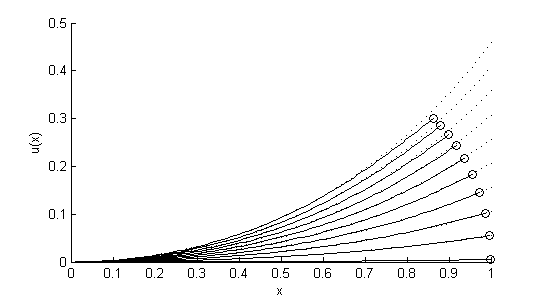
\includegraphics[width=0.60\textwidth]{./figures/lengthCorrectionErrorGraph2.png}
\end{center}
\caption[Původní ohybová funkce]%
{Původní ohybová funkce $u(x)$ pro různé výchylky (tečkovaně) a ohybová funkce po provedení korekce (plná čára). Kolečka vyznačují koncové body korigované křivky.
\label{fig:bendCorrectionGraph}
}
\end{figure}


Jak je patrné z obrázku ~\ref{fig:bendCorrectionGraph}, chyba způsobená popsanou metodou je relativně malá a nemění charakter původní ohybové křivky.

Výše popsaným způsobem získáme však ohybovou funkci pracující ve 2D. Větev je ale třeba deformovat ve 3D. Za tímto účelem jsou aplikovány dvě výše popsané deformace v navzájem kolmých osách ($r$,$s$). 

\begin{figure}[!hbt]
\begin{center}
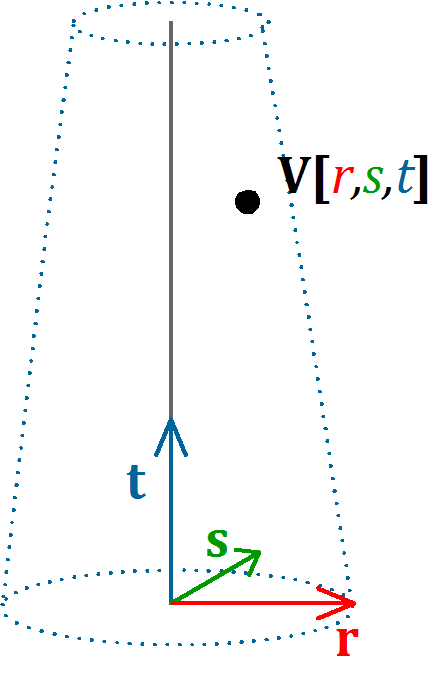
\includegraphics[width=0.2\textwidth]{./figures/branchCoords.png}
\end{center}
\caption[Souřadný systém větve]%
{Souřadný systém větve tvořený orthonormálními bázovými vektory $\vec{r}$, $\vec{s}$ a $\vec{t}$.
\label{fig:branchCoords}
}
\end{figure}

Jak vyplývá z Euler-Bernoulliho rovnice, síla ohýbající prut má lineární účinnek na ohybovou funkci – stačí tedy funkci $u(x)$ vynásobit silou $\vec{F}$, ohybová funkce závislá na síle působící na větev může být vyjádřena jako:
 \begin{equation}
\label{forceEq}
f(x) = |\vec{F}| \cdot u(x)
\end{equation}

Pokud připustíme, že síla určující výchylku je určitým řídícím signálem $A$, pak bude celková deformace řízena vztahem (indexy udávají, k jaké ose se daná funkce vztahuje):
\begin{equation}
\begin{array}{cc}
u_{r,s}(x) = A_{r,s}u(x) & {u}'_{r,s}(x) = A_{r,s}\frac{{u}'(x)}{L}
\end{array}
\end{equation}


Konečný tvar ohybové funkce pracující ve 3D je tudíž:
\begin{equation}
P = P_0 + \begin{pmatrix}
-d_r(x)/ s_r(x)-d_s(x)/s_s(x) \\ u_r(x)/s_r(x) \\ u_s(x)/s_s(x)
\end{pmatrix}
\end{equation}

Pro korektní zobrazování celé hierarchie větví je potřeba ještě správně transformovat normálu a tangentu v daném bodě $P$. Aby bylo možné korektně vyjádřit potřebné vektory, je nutné znát Jakobián $J_t$ popsané transformace. Bohužel právě jeho výpočet nelze efektivně provádět v real-time. Místo toho využijeme mnohem jednodušší Jakobián $J_u$ původní ohybové funkce (bez délkové korekce) a vyhodnotíme ho pro délkově korigovaný bod $P$.

\begin{equation}
J_{u} = \begin{pmatrix}
1 & 0 &0 \\
{u}'_r(x-d_r(x)/s_r(x)) & 1 & 0\\
{u}'_s(x-d_s(x)/s_s(x)) & 0 & 1\\
\end{pmatrix}
\end{equation}

Tangentu tedy vypočteme jako $\vec{t} = norm(J_{u}\vec{t}_{0})$, normálu pak jako $\vec{n} = norm(J_{u}^{-T}\vec{n}_{0})$

%%%%%%%%%%%%%%%%%%%%%%%%%%%%%%%%%%%%%%%%%%%%%%%%%%%%%%%%%%%%%%%%%
\subsection{Hierarchická deformace}

Předchozí kapitola popisuje, jak lze dosáhnout vcelku realistického ohybu osamocené větve. Je však třeba korektně propagovat deformaci do všech větví napojených. Pro rychlý a efektivní výpočet polohy každého vrcholu je nutné složit transformace vyplývající z topologie stromu (napojení větví a jejich ohyb). Pro každý vrchol je nutné mít přístupná data o relevantní části topologie, která ho ovlivňuje. K tomu stačí vědět, kde se větve oddělují ve smyslu parametru $x$ ohybové funkce (normovaná podélná vzdálenost na větvi). Každému vrcholu zavedeme tedy vektor hodnot $x$, kde $i$-tá složka vektoru odpovídá $i$-té hodnotě $x$ na cestě z kořene.
 
\begin{figure}[!hbt]
\begin{center}
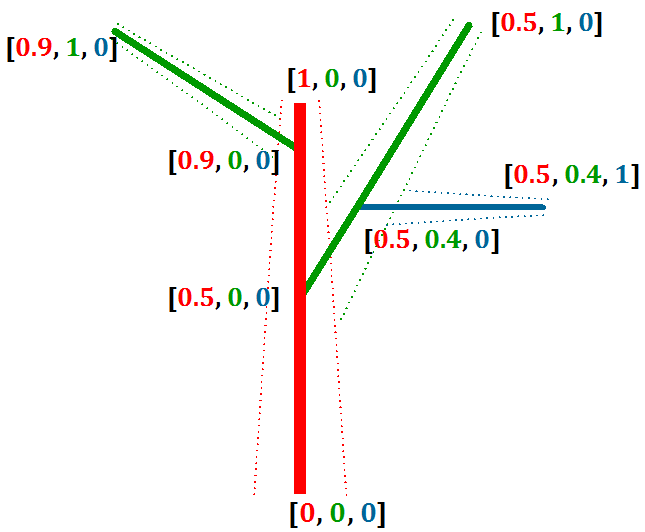
\includegraphics[width=0.5\textwidth]{./figures/branchHierarchy.png}
\end{center}
\caption[Vyjádření hierarchie]%
{ Vyjádření hierarchie pomocí vektoru s hodnotami $x$.
\label{fig:hierarchyCoords}
}
\end{figure}

Dále musí mít vrchol přiřazeny souřadnice $r$, $s$, $t$ v souřadné soustavě větve.
\begin{figure}[!hbt]
\begin{center}
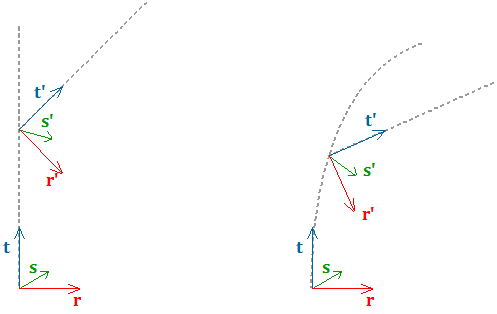
\includegraphics[width=0.5\textwidth]{./figures/coordTransf.png}
\end{center}
\caption{ Souřadný systém větve a jeho transformace při ohybu nadřazené větve
\label{fig:transfCoordSys}
}
\end{figure}	 
Aby se při ohýbání větev nezplošťovala, je nutné provádět transformaci souřadného systému větve pro každý vrchol. Zde je možnost tuto korekci neprovádět a zrychlit tak výpočet na úkor kvality výsledného ohybu.

	 
\begin{figure}[!hbt]
\begin{center}
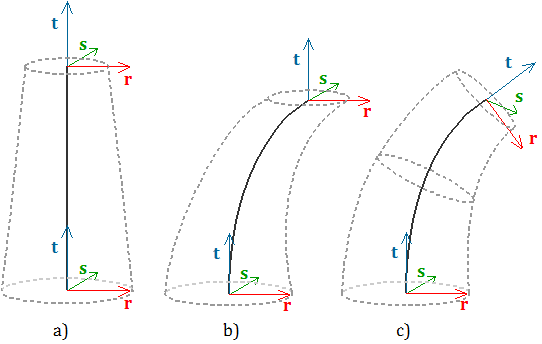
\includegraphics[width=0.5\textwidth]{./figures/branchBend.png}
\end{center}
\caption[Transformace souřadných systémů při ohybu]%
{Transformace souřadných systémů při ohybu.
(a) výchozí poloha, (b) ohyb bez transformace souřadného systému, (c) ohyb se správnou transformací
\label{fig:bendCoordSys}
}
\end{figure}

Jak je patrné z obrázku ~\ref{fig:bendCoordSys}, při malých deformacích je chyba v podstatě zanedbatelná. Při výpočtu polohy bodu $\vec{p_i}$ na středovém paprsku větve je vhodné použít následujících iterativních vztahů:

\begin{align} 
\vec{p}_{i} &= \vec{p}_{0} - \frac{\vec{t}d_{r}(x)-\vec{r}u_{r}(x)}{s_{r}(x)}-\frac{\vec{t}d_{s}(x)-\vec{s}u_{s}(x)}{s_{s}(x)}\nonumber\\
x_{i,r,s} &= x - \frac{d_{r,s}(x)}{s_{r,s}(x)}\nonumber\\
\vec{t}_{i} &=  \vec{t}_{0} + (u'_{r}(x_{i,r})\vec{r} + u'_{s}(x_{i,s})\vec{s})(\vec{t}\cdot\vec{t}_{0})\\
\vec{n}_{i} &=  \vec{n}_{0} + (u'_{r}(x_{i,r})(\vec{r} \cdot \vec{n}_{0}) + u'_{s}(x_{i,s})(\vec{s} \cdot \vec{n}_{0})\vec{t}
\end{align}

Pokud výpočet transformace polohy bodu bude probíhat od kořene hierarchie, dokud v ní není dosaženo úrovně, na které se daný vrchol nachází, pak budou postupně aplikovány všechny relevantní deformace. Na počátku je $\vec{p_0}$ původní poloha bodu v souřadném systému objektu (obdobně i tečna $\vec{t_0}$  a normála $\vec{n_0}$). V každé další iteraci (postupu o úroveň výš v hierarchii) je třeba počáteční vektory $\vec{p_0}$, $\vec{t_0}$ a $\vec{n_0}$ nastavit na výsledek z předchozí iterace. Hodnota $x_{D,r}$ a $x_{D,s}$ představuje hodnotu parametru $x$ po provedení korekce délky.  Transformace souřadného systému v rámci jedné větve vyžaduje přepočet nového bázového vektoru $\vec{t}$ podle vzorce pro výpočet tečny a nových bázových vektorů $\vec{r}$ a $\vec{s}$ podle vzorce pro výpočet normály. 

Následující tabulka shrnuje, jaká data jsou potřeba pro výpočet deformace:

\begin{table}[here]
\centering
\begin{tabular}{| l | l | }
  \hline                       
  pro vrchol & pro celou větev  \\
\hline   
  skutečná poloha & koeficienty $c_2$,  $c_4$ , délka  $L$  \\
  poloha vzhledem k větvi & definice souřadného systému větve \\
hodnota x na větvi & řídící signály ohybu \\
odkaz na větevi & odkaz na nadřazenou větev \\
  \hline  
\end{tabular}
\caption{Data potřebná k výpočtu hierarchické deformace větve}
\end{table}


%%%%%%%%%%%%%%%%%%%%%%%%%%%%%%%%%%%%%%%%%%%%%%%%%%%%%%%%%%%%%%%%
\subsection{Deformace listů}
Listy jsou součástí hierarchie stromu a musí proto respektovat i příslušný řetěz deformací této hierarchie. Kromě toho ovšem přidávají i vlastní deformaci, která je svou podstatou odlišná od deformace větví. Uplatňuje se tu jak podélná deformace, tak krut, který nastavuje plochu listu do rovnovážné polohy vzhledem k mechanickým vlastnostem a působícímu větru. 
\begin{figure}[here]
\begin{center}
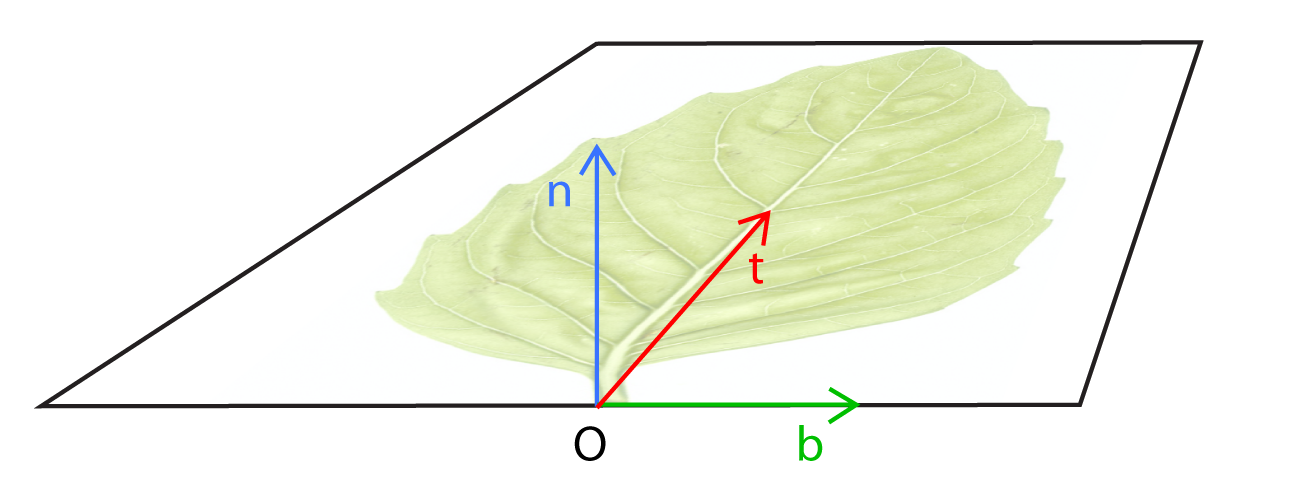
\includegraphics[width=0.45\textwidth]{./figures/leafCoordSystem2.png}
\end{center}
\caption[Souřadný systém listu]%
{ Souřadný systém listu.
\label{fig:bendLeaf}
}

\end{figure}
Jelikož považujeme listy za velice lehké a v rámci své plochy za nedeformovatelné, je tedy deformace listu aproximována jako orientace plochy listu vůči větvi, ze které vyrůstá. Jde tedy o relativně primitivní transformaci souřadného systému listu, který vytvoříme způsobem naznačeným na obrázku ~\ref{fig:bendLeaf}.


Deformace listu pak může probíhat takto:
\begin{align*} 
\vec{t}_t &= \vec{t}_0 + \vec{n}_0*A_x\\
\vec{n}_t &= \vec{t}_t \times \vec{b}_0\\
\vec{n}_r &= \vec{n}_t + \vec{b}_0*A_y\\
\vec{b}_r &= \vec{t}_t \times \vec{n}_r\\
\vec{t}_r &= \vec{t}_t
\end{align*}
\newline
\begin{equation}
P_d = O_{xyz} + P_x*\vec{b}_r + P_y*\vec{t}_r
\end{equation}
Bod $O$ je místo, kde se list napojuje na větev souřadnice $P_x$ a $P_y$ jsou dány relativně, vůči tomuto bodu v soustavě $\vec{n}\vec{b}\vec{t}$.


%%%%%%%%%%%%%%%%%%%%%%%%%%%%%%%%%%%%%%%%%%%%%%%%%%%%%%%%%%%%%%%%%%%
\subsection{Řízení animace}

Animace by měla uživateli navodit dojem, že se strom hýbe působením větru. Uvažujme, že celý pohyb je způsoben hledáním rovnovážné polohy, která závisí na mechanických vlastnostech stromu a vnějších sil (gravitace a vítr). Tím, že vnější síla v podobě působení větru je značně proměnlivá, dochází k neustálému neuspořádanému kývání kolem tušené rovnovážné polohy. Pro účely této práce dále uvažujme, že má vítr určitou složku směrového proudění  a složku turbulentního proudění. Zmíněné nahodilé kývání zřejmě způsobuje turbulentní složka, zatímco složka směrového proudění má spíše za následek celkovou změnu rovnovážné polohy (pozorovatel vnímá, že se celý strom ohýbá). 

Pozorujeme-li reálný strom, pak pro určité rozmezí malé síly větru nelze určit, kterým směrem vítr vane. V takovém případě tedy výrazně převládá vliv turbulentní složky. Lze však sledovat, že čím je daná větev větší, tím je frekvence těchto výkyvů nižší a amplituda naopak vyšší. Velikost větve odpovídá vcelku dobře její úrovni v hierarchii větví. 

Naproti tomu silnější vítr způsobí celkové ohnutí stromu do směru, kam vane. Převládá složka směrového proudění. Frekvence výkyvů jednotlivých větví se zvyšuje. Do určité meze roste i amplituda. Po jejím překročení amplituda klesá. V případě extrémní síly větru je již nahodilý pohyb větví vlivem působících sil minimální.

Popis deformací z kapitoly ~\nameref{sec-branchDeformation}  umožňuje jednoduše zohlednit obě zmiňované působící složky.
Vyjdeme-li ze vztahu \eqref{forceEq} a rozvineme sílu $\vec{F}$ do tvaru:
\begin{equation}
\label{windEq}
F_{d} = \left | \vec{W}_{turb} \right | + \vec{d}\cdot \vec{W}_{lin}
\end{equation}
bude možné promítnout sílu směrové složky větru $\vec{W}_{lin}$ a turbulentní složky $\vec{W}_{turb}$ do směru $\vec{d}$ resp. do směrů $\vec{r}$, $\vec{s}$. Aby bylo možné dosáhnout kýženého efektu způsobeného turbulentní složkou, je třeba v čase měnit příslušným způsobem sílu $\vec{W}_{turb}$. Obě složky lze chápat jako řídící signály animace (směrová složka může zůstávat konstantní). Jsou-li tyto signály měněny plynule, je plynulá i výsledná animace.

Jednotlivé větve je však třeba řídit vzájemně nezávislými signály. Proto je nutné generovat pro každou větev dvousložkový šum, který bude ideálně aperiodický a pro větev unikátní. S přihlédnutím k možnostem grafického hardwaru se jako velmi výhodná jeví strategie využívající jedinou šumovou texturu pro generování celé třídy řídících šumových funkcí. Vyhodnocením vzorku dat na určité pozici získáváme vlastně funkční hodnotu. Bude-li se pozice v textuře plynutím času posouvat po přímce definované směrovým vektorem $\vec{mv}$ (popřípadě i počátečním bodem $o$), získáme postupně funkční hodnoty průběhu požadované šumové funkce. Vzorek dat pak může obsahovat více kanálů (např. RGB, jak je u obrázků běžné) a získáme takto i více různých šumových funkcí současně, jak je patrné na obrázku \ref{fig:noiseFunctions} .
 \begin{figure}[here]
\begin{center}
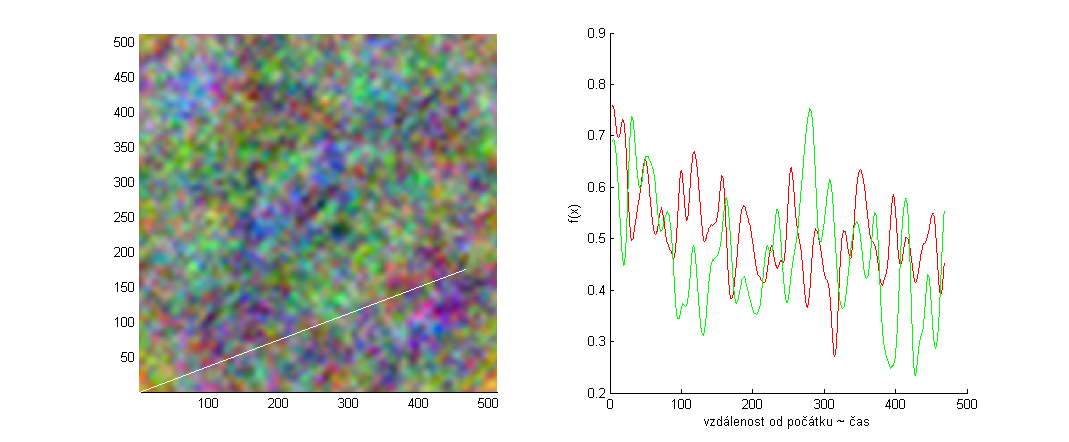
\includegraphics[width=0.85\textwidth]{./figures/noiseCut1.png}
\end{center}
\caption[Dvě generované šumové funkce]%
{ Dvě generované šumové funkce pro červený a zelený kanál (vlevo) získané odečítáním hodnot na bílé úsečce v šumové textuře (vpravo) \label{fig:noiseFunctions}
}

\end{figure}

\pagebreak
Pro pozorovatele jsou jednotlivé řídící funkce větví nezávislé – turbulentní složka je pro pozorovatele natolik chaotická, že nemůže lehce určit vzájemné vazby. Naproti tomu pro listy, které svým chováním vlastně přímo vzorkují turbulentní proudění, je dobré dodržet určité prostorové vazby. Pozorovatel totiž dokáže rozeznat poryv větru docela dobře podle pohybu listů. Listy v blízkém okolí musí na poryv reagovat podobně. Z toho důvodu zavedeme zjednodušený model turbulentního pole (viz obrázek ~\ref{fig:TurbulentFieldModel}). 
\begin{figure}[!hbt]
\begin{center}
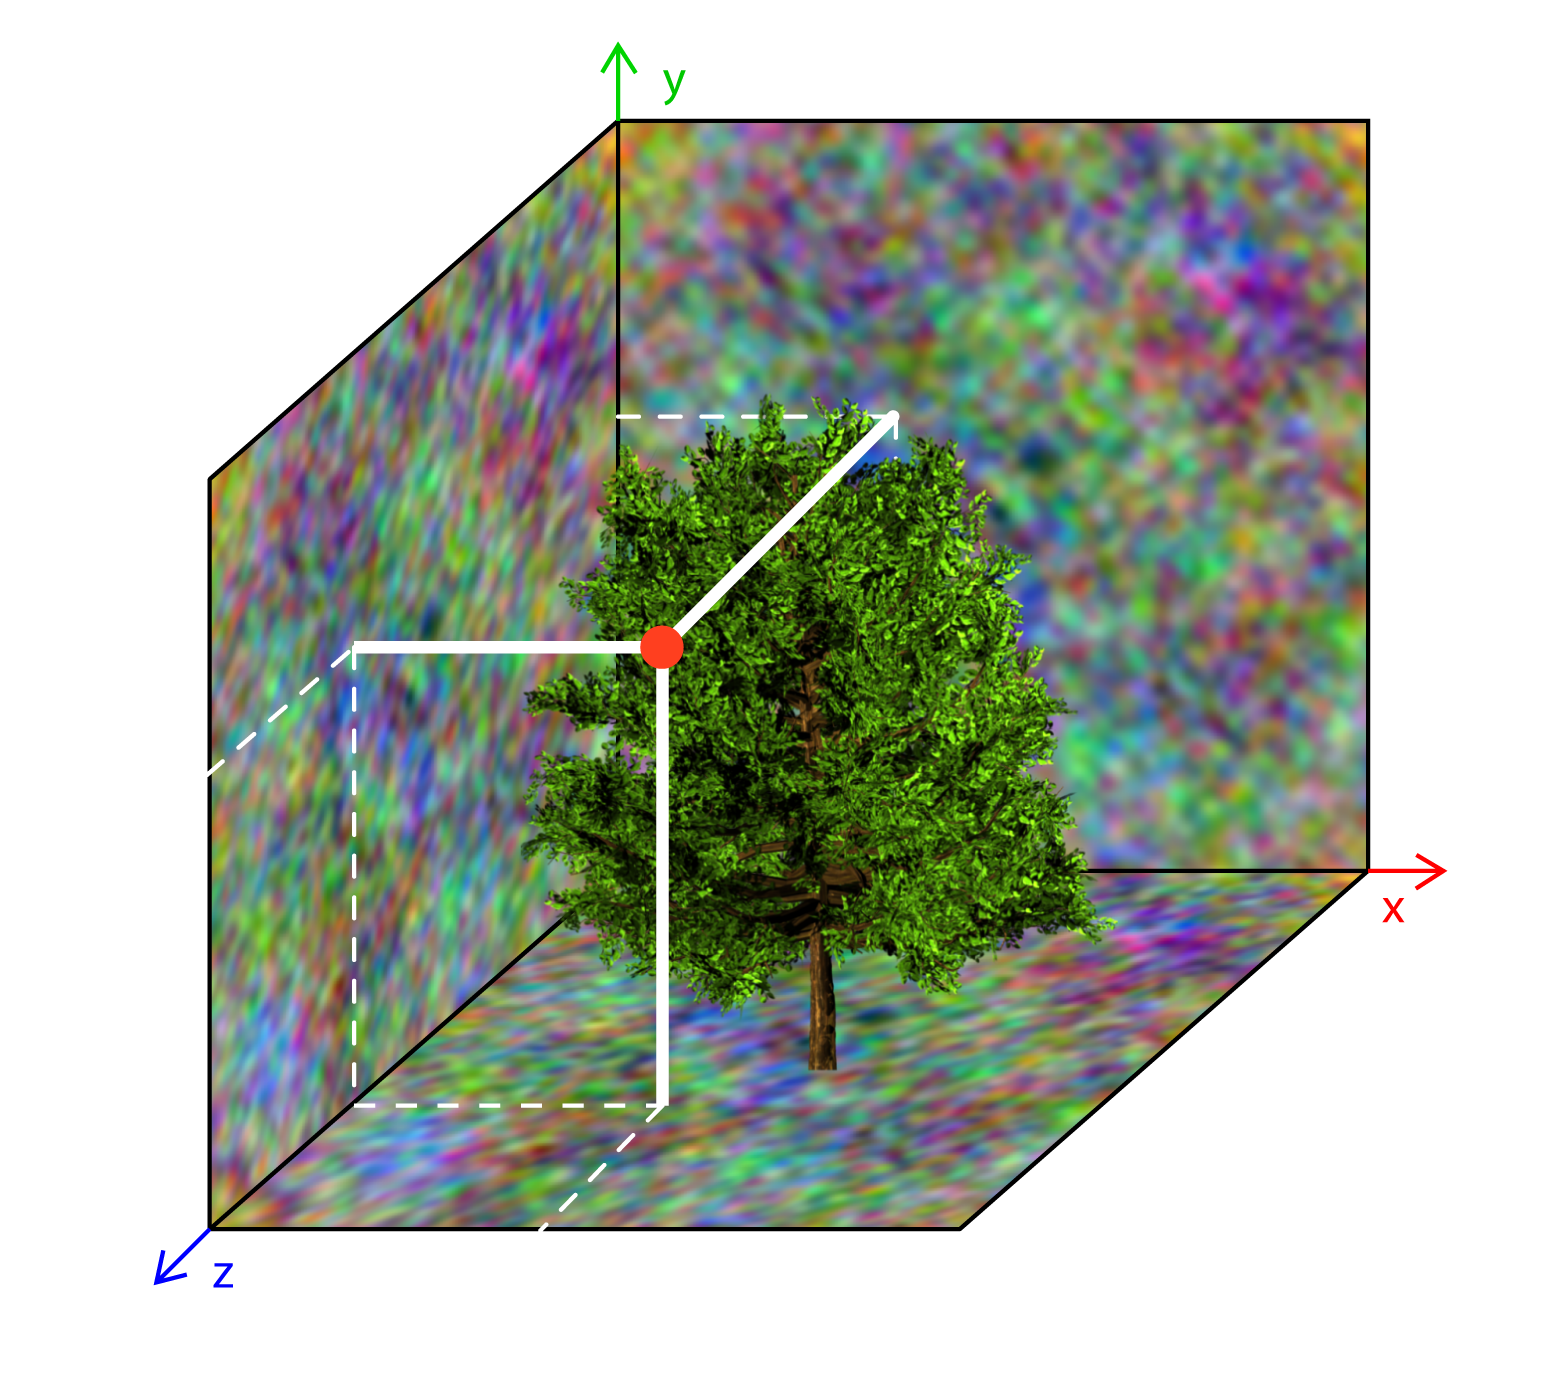
\includegraphics[width=0.5\textwidth]{./figures/turbulentField.png}
\caption[Model 3D turbulentního pole]%
{Model 3D turbulentního pole pro animaci listů\label{fig:TurbulentFieldModel}}
\end{center}

\end{figure}

 K tomu lze využít jedinou šumovou texturu. Pozici dotazu do turbulentního pole posuneme o vektor $-\vec{W} \cdot t$, kde $t$ je čas. Získáme tak 3 hodnoty $A_{xy,xz,yz}$, ze kterých vypočteme vážený součet. 
\begin{equation}
 A^{l} = A^p_{xy}(1-\frac{\left | W_z\right |}{\left | \vec{W}\right |})
+ A^p_{yz}(1-\frac{\left | W_x\right |}{\left | \vec{W}\right |}) +
A^p_{xz}(1-\frac{\left | W_y\right |}{\left | \vec{W}\right |})
\end{equation}
Výsledkem je hodnota, která je největším dílem tvořena z roviny, jež nejlépe odpovídá směru větru.


% Zobrazování listů %%%%%%%%%%%%%%%%%%%%%%%%%%%%%%%%%%%%%%%%%%%%%%%%%%%
\section{Zobrazování listů}
\label{sec-leafMethod}
Listy rostlin představují z hlediska počítačové grafiky zajímavý objekt. Jejich vizuální vlastnosti se liší mezi jednotlivými druhy rostlin. Zároveň je často velmi markantní rozdíl mezi rubovou (horní) a lícovou (spodní) stranou. Zatímco zvrchu jsou některé listy vysoce lesklé díky různým voskovým vrstvičkám, zespodu jsou často spíše matné. Některé listy mají na povrchu miniaturní chloupky, které jim dávají hedvábný vzhled. Dalšími faktory jsou pak tvar, tloušťka a barva listu. 
 \begin{figure}[here]
\begin{center}
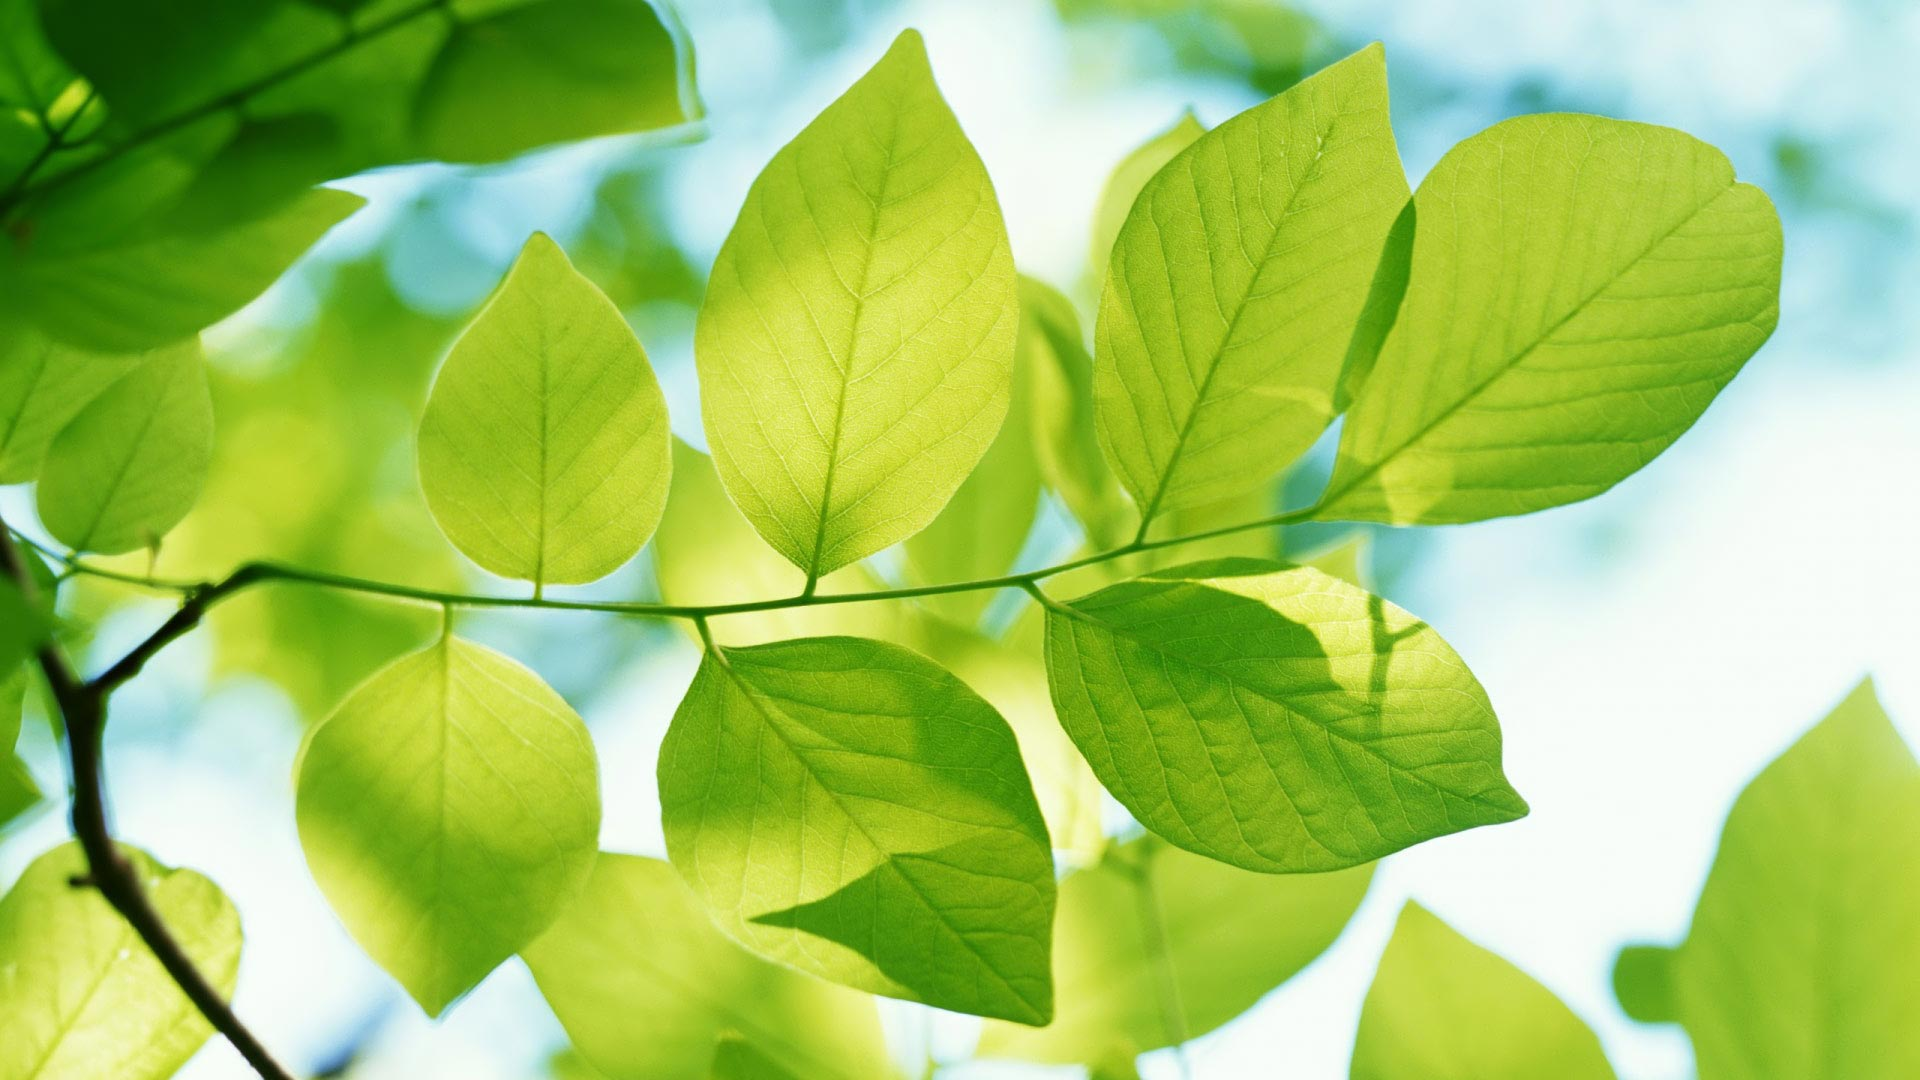
\includegraphics[width=0.5\textwidth]{./figures/translucent_leaves.jpg}
\end{center}
\caption{ Fotografie skutečných listů, kde se projevuje jejich průsvitnost, zdroj \cite{TLW} \label{fig:translucentLeaves}
}

\end{figure}

Metod a postupů, jak zobrazovat listy v real-time existuje několik. Většina přístupů se ale spokojuje s tím, že bere v potaz pouze povrchové vlastnosti listu a simuluje tak například členitost jeho povrchu či běžné odrazové vlastnosti. Metoda popsaná v \cite{Habel_2007_RTT} ovšem zahrnuje i průsvitnost listů, která hraje zásadní roli zejména na spodní straně listu (viz obr. \ref{fig:translucentLeaves}). Osvětlení listu lze zformulovat do následujícího vztahu
\begin{equation}
L = L_D + L_I + L_E,
\end{equation}
kde výsledné osvětlení $L$ z jednoho světelného zdroje se skládá z příspěvku přímého ($L_D$) a nepřímého ($L_I$) osvětlení a složky $L_E$, kterou list emituje. 
V následujícím textu bude rozebrán pouze příspěvek přímého osvětlení. Zbylé budou aproximovány ambientní složkou. Přímé osvětlení lze pak schematicky rozepsat jako:
\begin{equation}
\label{eq:directLight}
L_D = L_{diffuse} + L_{specular}+ L_{ambient} + L_{translucent},
\end{equation}
kde první tři členy představují příspěvek odraženého světla, zatímco poslední člen $ L_{translucent}$ se vztahuje k průsvitnosti listu.

K vyjádření difuzní a spekulární složky využijeme popisu z obrázku \ref{fig:lightModel}.
 \begin{figure}[here]
\begin{center}
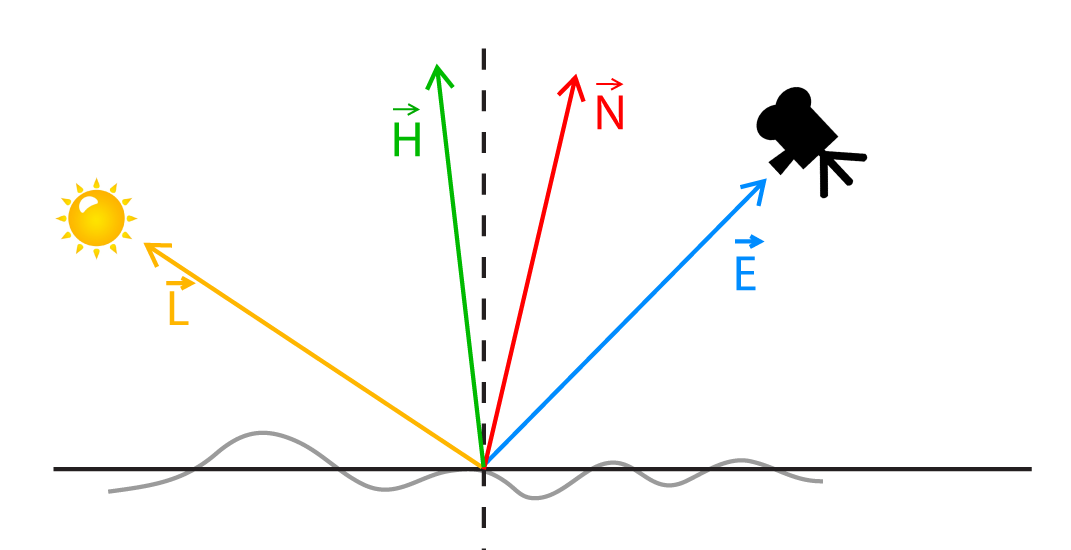
\includegraphics[width=0.5\textwidth]{./figures/lightModel.png}
\end{center}
\caption[Situace na povrchu listu]
{Situace na povrchu listu.  Vektor $\vec{N}$ definuje normálu v bodě dopadu paprsku. $\vec{E}$ udává směr k pozorovateli a $\vec{L}$ ke světlu. Vektor $\vec{H}$ je definován na ose úhlu mezi $\vec{L}$ a $\vec{E}$. Šedivá křivka představuje povrch.\label{fig:lightModel}
}
\end{figure}
Difuzní složku lze určit jako příspěvek světla vážený úhlem mezi přicházejícím paprskem světla $\vec{L}$ a normálou povrchu $\vec{N}$ v místě jeho dopadu:
\begin{equation}
L_{diffuse} = \vec{N} \cdot \vec{L}
\end{equation}
Výpočet spekulární složky je oproti tomu složitější. Nevyužívá Phongova osvětlovacího modelu, ale nahrazuje ho odvozeninou osvětlovacího modelu Cook-Torrance popsaného v \cite{Cook:1981:RMC:965161.806819} a \cite{Bousquet2005201}. Tento model pracuje s BRDF jež operuje nad proměnými $\vec{N}$, $\vec{L}$, $\vec{E}$, $\vec{H}$ (význam viz obr. \ref{fig:lightModel}), $\sigma$ udávajícím drsnost povrchu a indexem lomu $n$ světla na povrchu listu.

\begin{equation}
\label{eq:brdf}
BRDF_{spec}(\vec{N}, \vec{L}, \vec{E}, \vec{H}, \sigma, n) = \frac{R(\sigma, \vec{N}, \vec{H}) \cdot F(n, \vec{H}, \vec{E}) \cdot G(\vec{N}, \vec{L}, \vec{E},\vec{H}) }{(\vec{N}\cdot\vec{L})(\vec{N}\cdot\vec{E})\pi}
\end{equation}
Člen $R(\sigma, \vec{N}, \vec{H})$ představuje vliv hrubosti povrchu a může být vyjádřen jako:
\begin{equation}
\label{eq:roughness}
R(\sigma, \vec{N}, \vec{H}) = \frac{1}{\sigma^2 \cdot ( \vec{N}\cdot\vec{H})^4} \cdot e^{\left ( \frac{\frac{1}{ ( \vec{N}\cdot\vec{H})^2} -1}{\sigma^2}\right )}
\end{equation}
Naproti tomu, člen $F(n, \vec{H}, \vec{E})$ popisuje lesklou složku:
\begin{align}
\label{eq:fresnel}
c &= \vec{H} \cdot \vec{E} \nonumber\\
g &= \sqrt{n^2 + c^2 - 1}\nonumber\\
F(n, \vec{H}, \vec{E}) &= \frac{1}{2} \left ( \frac{g-c}{g+c} \right)^2 \left [  1+ \left( \frac{c (g+c)-1}{c(g-c)+1}\right)\right ]
\end{align}
Konečně člen $G(\vec{N}, \vec{L}, \vec{E},\vec{H})$ popisuje geometrii v bodě dopadu paprsku:
\begin{equation}
\label{eq:geometry}
G(\vec{N}, \vec{L}, \vec{E},\vec{H}) = \min{} \left( 1, \frac{2\cdot(\vec{N}\cdot\vec{H})\cdot(\vec{N}\cdot\vec{E})}{(\vec{E}\cdot\vec{H})}, \frac{2\cdot(\vec{N}\cdot\vec{H})\cdot(\vec{N}\cdot\vec{L})}{(\vec{E}\cdot\vec{H})} \right)
\end{equation}

Složka způsobená průsvitností listu má dominantní vliv, pokud se světelný zdroj nachází za rovinou listu vzhledem k pozorovateli. K jejímu vyjádření je použit BSSRDF model. Jeho konstrukcí a určením pro různé listy se věnuje \cite{Habel_2007_RTT} a tato problematika zde nebude dále rozebírána. Zmiňovaná funkce $L_t$ závisí na pozici $\vec{x}_0$, směru k pozorovateli $\vec{E}$ a směru ke světlu $\vec{L}$ a může být napsána v diskrétní formě takto:
\begin{equation}
\label{eq:bssrdf}
L_t(\vec{x}_0, \vec{E}, \vec{L}) = \rho_t(\vec{x}_0, \vec{E}) A_p \sum\limits_{\vec{x}_i} T(r, d(\vec{x}_i))E(\vec{x}_i, \vec{L}),
\end{equation}
kde $\rho_t(\vec{x}_0, \vec{E})$ reprezentuje propustnost, $A_p$ zastupuje plochu texelu, $T(r, d(\vec{x}_i))$ je dynamické konvoluční jádro díky závislosti na tloušťce listu $d(\vec{x}_i)$ a konečně $E(\vec{x}_i, \vec{L})$ je přenosová funkce osvitu (irradiance transport function). Jde v zásadě o proces konvoluce obrazové informace a můžeme tedy odlišit konvoluční část.
\begin{align}
\label{eq:bssrdf_convol}
L_t(\vec{x}_0, \vec{E}, \vec{L}) &= \rho_t(\vec{x}_0, \vec{E}) L_t^C( \vec{x}_0, \vec{L}) \\
L_t^C( \vec{x}_0, \vec{L})  &= A_p \sum\limits_{\vec{x}_i} T(r, d(\vec{x}_i))E(\vec{x}_i, \vec{L}),
\end{align}
 Právě konvoluční část tvořená hemisférickou funkcí $L_t^C$ je v real-time příliš obtížné vypočíst, a proto se předpočítá pro každý texel. Reprezentována pak je pomocí tzv. \emph{Half Life 2 bází} (HL2b). Jde o konstrukt, který umožňuje jednoduše vyjádřit reprezentovanou funkci pro daný hemisférický směr. Bázové vektory HL2b jsou následující:
\begin{align}
\label{eq:hl2b_vectors}
\vec{H}_1 &= (-\frac{1}{\sqrt{6}}, -\frac{1}{\sqrt{2}}, \frac{1}{\sqrt{3}}) \nonumber\\
\vec{H}_2 &= (-\frac{1}{\sqrt{6}}, \frac{1}{\sqrt{2}}, \frac{1}{\sqrt{3}}) \nonumber \\
\vec{H}_3 &= (\sqrt{\frac{2}{3}}, 0, \frac{1}{\sqrt{3}})
\end{align}
Tyto vektory pak definují tři kosínové bázové funkce na polokouli (hemisféře):
\begin{equation}
\label{eq:hl2b_cosineFunctions}
\mathcal{H}_i(\vec{d}) = \sqrt{\frac{3}{2\pi}}\vec{H}_i \cdot \vec{d}
\end{equation}
Hemisférickou funkci $f(\vec{d})$ pro směr $\vec{d}$  lze tedy přepsat pomocí těchto bázových funkcí následovně:

\begin{equation}
\label{eq:hl2b_function}
f(\vec{d}) = \sum\limits_{i=1\dots3}h_i\mathcal{H}_i(\vec{d}),
\end{equation}
kde $h_i$ jsou souřadnice vzhledem k bázovým funkcím.

Výsledný vztah rekonstruující původní $L_t$ využívající HL2b pro předpočítanou konvoluční funkci pak vypadá takto:
\begin{equation}
\label{eq:hl2b_use}
L_t^R(\vec{x}_0, \vec{L}) = L_D \rho(\vec{x}_0) \sum\limits_{i=1\dots3}h_i(\vec{x}_0)\sqrt{\frac{3}{2\pi}}\vec{H}_i \cdot  \vec{L}
\end{equation}
Uvážíme-li, že $L_D \rho(\vec{x}_0)$ a $h_{1\dots3}(\vec{x}_0)$ lze uložit do textur (pro pozici $\vec{x}_0$), lze tím pádem průsvitnost vypočíst na základě pouze dvou dotazů do textur.

Posledním krokem je přizpůsobit výše popsané postupy tak, aby bylo možné dynamicky měnit barvu listů. Barva se liší jednak v rámci jednoho listu, jednak mezi listy. Sezónní změny barvy listu se často projevují různě v různých částech listu. Zatímco okrajové části mohou být už červené či žluté, středové části mohou zůstávat stále zelené. Toto chování ovšem není cílem napodobit. Důraz bude kladen na celkovou barevnost listu, která hraje roli při pohledu z větší vzdálenosti.
\begin{figure}[here]
\begin{center}
$\begin{array}{cc}
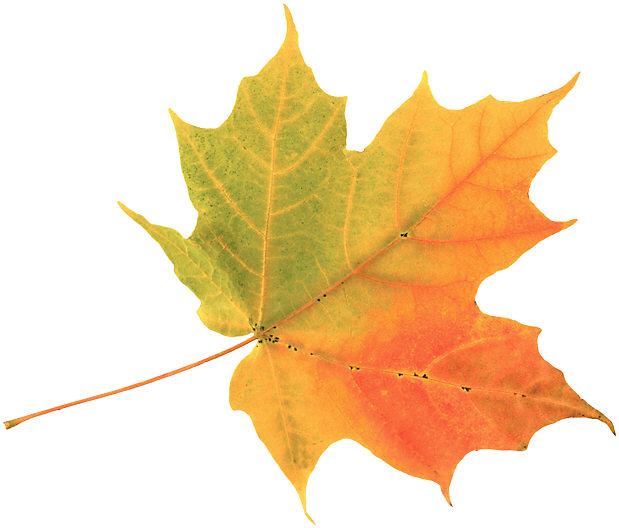
\includegraphics[width=0.4\textwidth]{./figures/fall-leaf.jpg}&
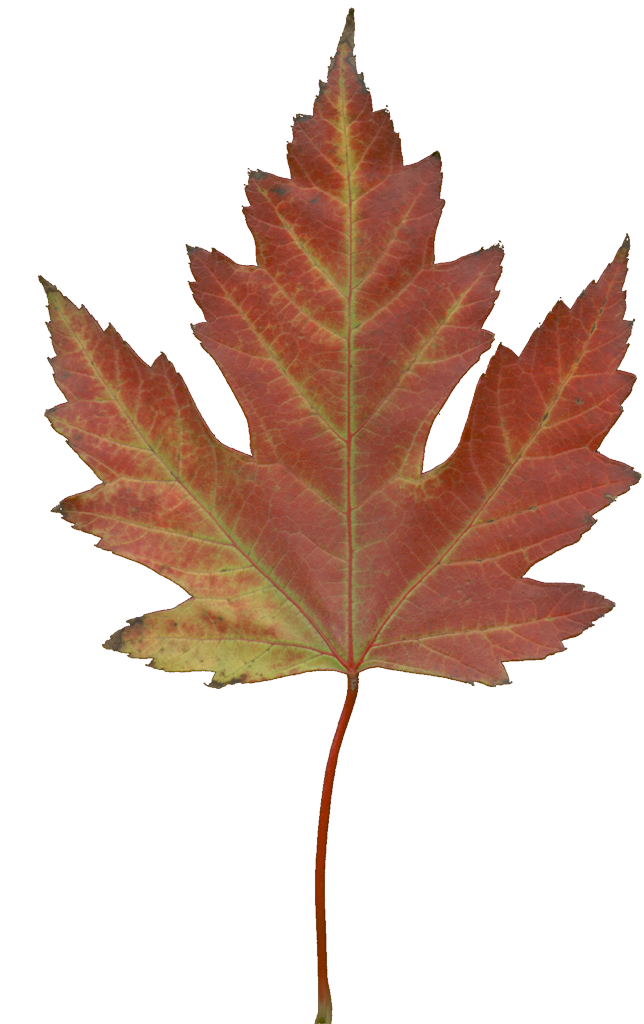
\includegraphics[width=0.3\textwidth]{./figures/fall-leaf2.png}
\\
(a)&(b)
\end{array}$
\end{center}
\caption{ Fotografie skutečných listů, barevné variace v ploče listu\label{fig:fallLeaves}
}
\end{figure}

Vyjdeme-li ze vztahu \ref{eq:directLight}, a budeme-li ho chápat pouze jako jednotlivé skalární podíly intenzit světla, můžeme vytvořit následující vztah pro zahrnutí barevnosti listu: 
\begin{equation}
\label{eq:color_solution}
L_D = L_{diffuse}  \mathcal{D} + L_{specular} \mathcal{S} + L_{ambient} \mathcal{A}   + L_{translucent} \mathcal{T} ,
\end{equation}
přičemž $\mathcal{D}$ je difuzní barva v daném bodě, $\mathcal{S}$ je barva odlesku daná barvou světelného zdroje a materiálem, $\mathcal{A}$ je barva ambientního příspěvku světla a $\mathcal{T}$ je barva vzniklá průchodem světla listem.

 Pro konkrétní bod $x$ a sezónu $s$ lze barvy vyjádřit jako:
\begin{align}
\label{eq:color_def}
\mathcal{D}(x,s) &= (c_v(x) + c_s(s))\cdot \mathcal{M}_{diffuse}\nonumber\\
\mathcal{A}(x,s) &= (c_v(x) + c_s(s))\cdot \mathcal{M}_{ambient}\nonumber\\
\mathcal{S}(x,s) &= \mathcal{M}_{specular}\nonumber\\
\mathcal{T}(x,s) &= (c_t(x) + c_s(s))\cdot \mathcal{M}_{translucent} ,
\end{align}
kde $ \mathcal{M}_{(\dots)}$ je pro daný materiál na světelný zdroj konstanta, $c_v(x)$ je prostá barva listu, která je definovaná texturou, $c_s(x)$ je barevná odchylka daná sezónními změnami barvy (dovolíme si zjednodušení: sezónní barevná odchylka je pro celý list stejná ). Člen $c_t(x)$ vyjadřuje barvu po průchodu světla listem, která je rovněž definovaná texturou. Na tomto místě je dobré přiznat, že správnější by bylo uvažovat pro různé barevné variace listu dané sezónou i různé barvy průsvitné složky. Řešní by se tím ovšem zkomplikovalo a i popsaný přístup funguje relativně dobře.
Předpokládá se, že každá ze dvou stran listu bude vyhodnocována odděleně s jinými parametry (různé textury, příp. materiály). Na obrázku \ref{fig:leafResources} jsou zdrojové textury pro jednu stranu listu.
\begin{figure}[here]
$\begin{array}{cccc}
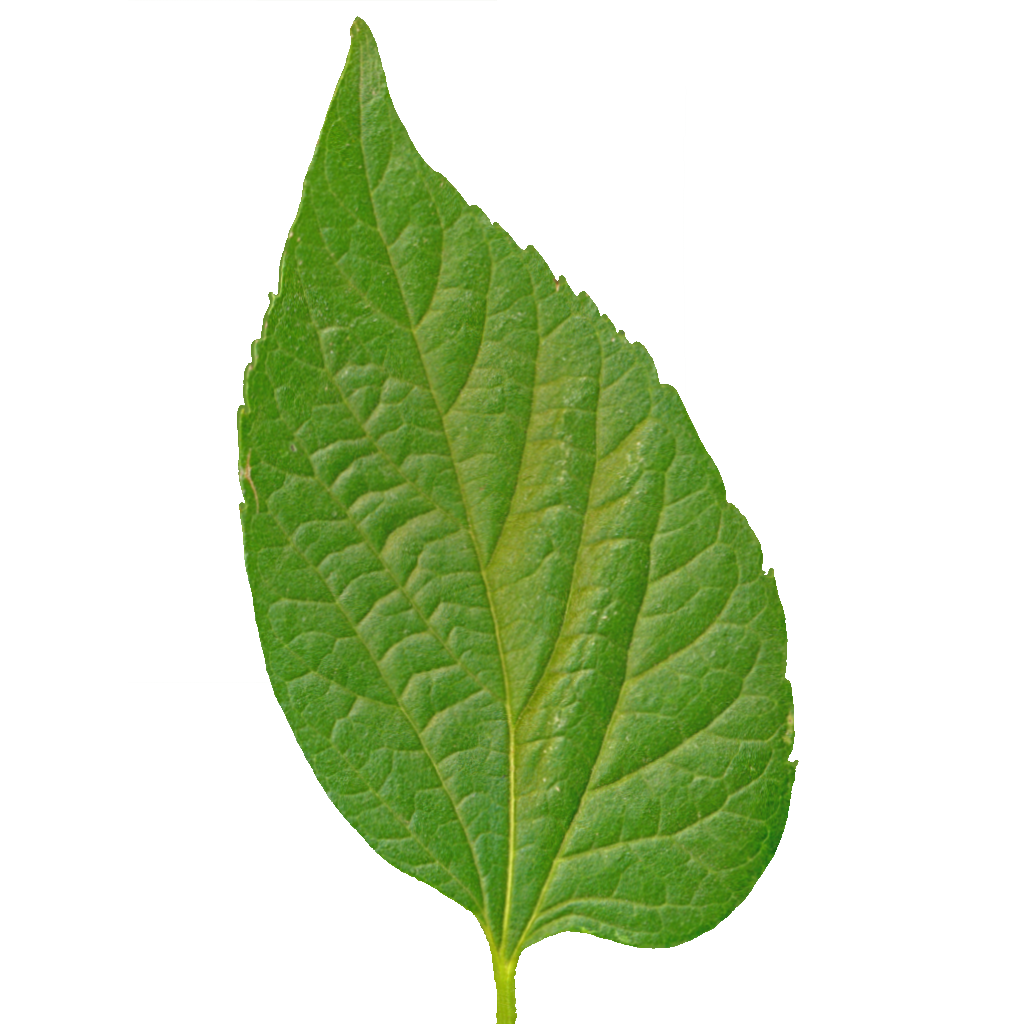
\includegraphics[width=0.2\textwidth]{./figures/leaf3_decal_front.png}&
&
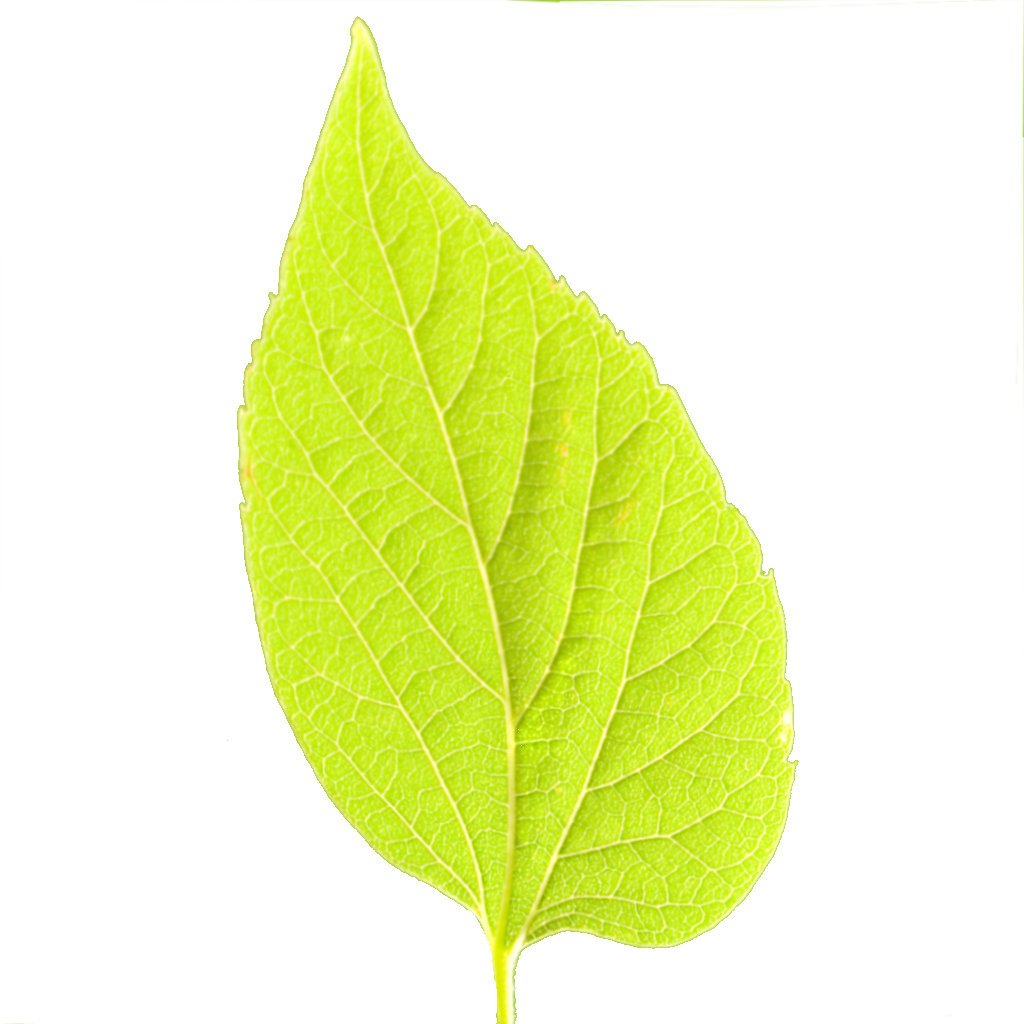
\includegraphics[width=0.2\textwidth]{./figures/leaf3_translucency_front.png}&
\\
(a)&&(b)&
\\
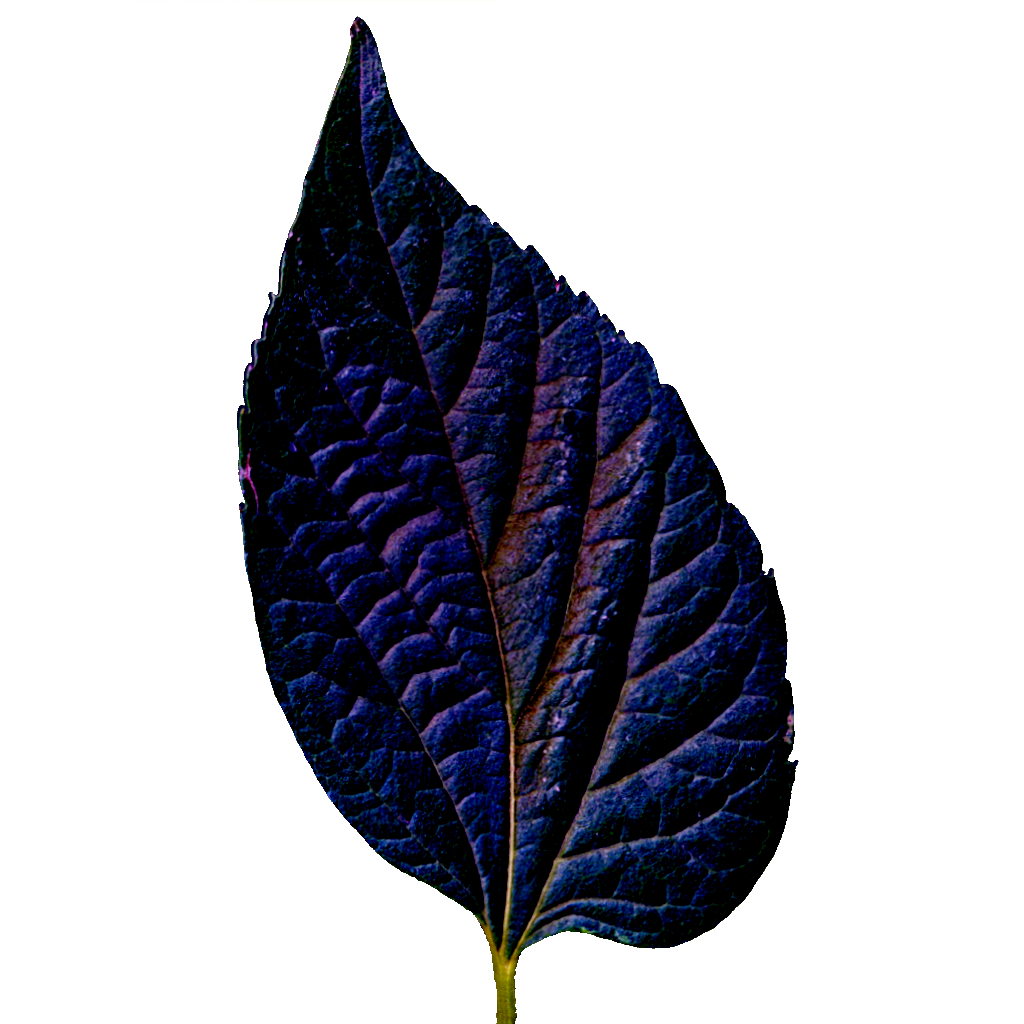
\includegraphics[width=0.2\textwidth]{./figures/leaf3_decal_front_e.png}&
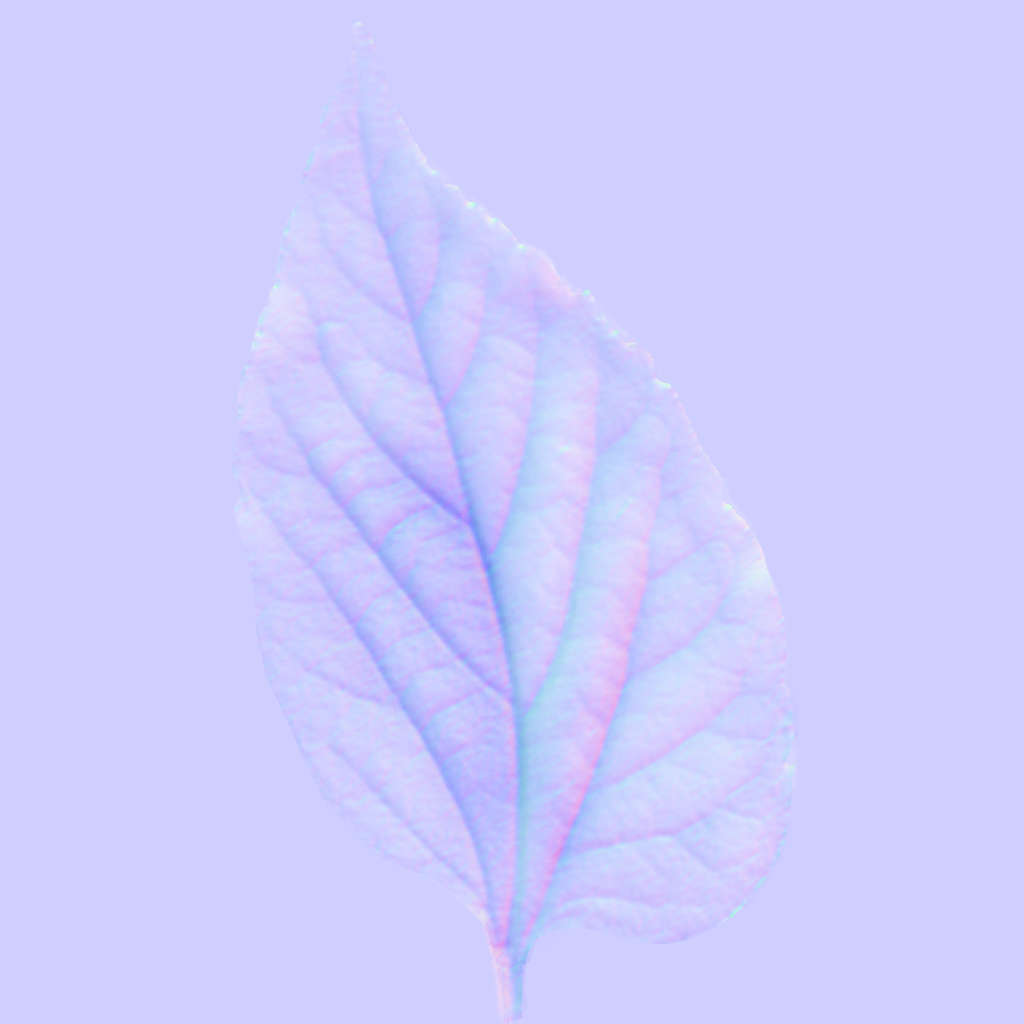
\includegraphics[width=0.2\textwidth]{./figures/leaf3_normal_front.png}&
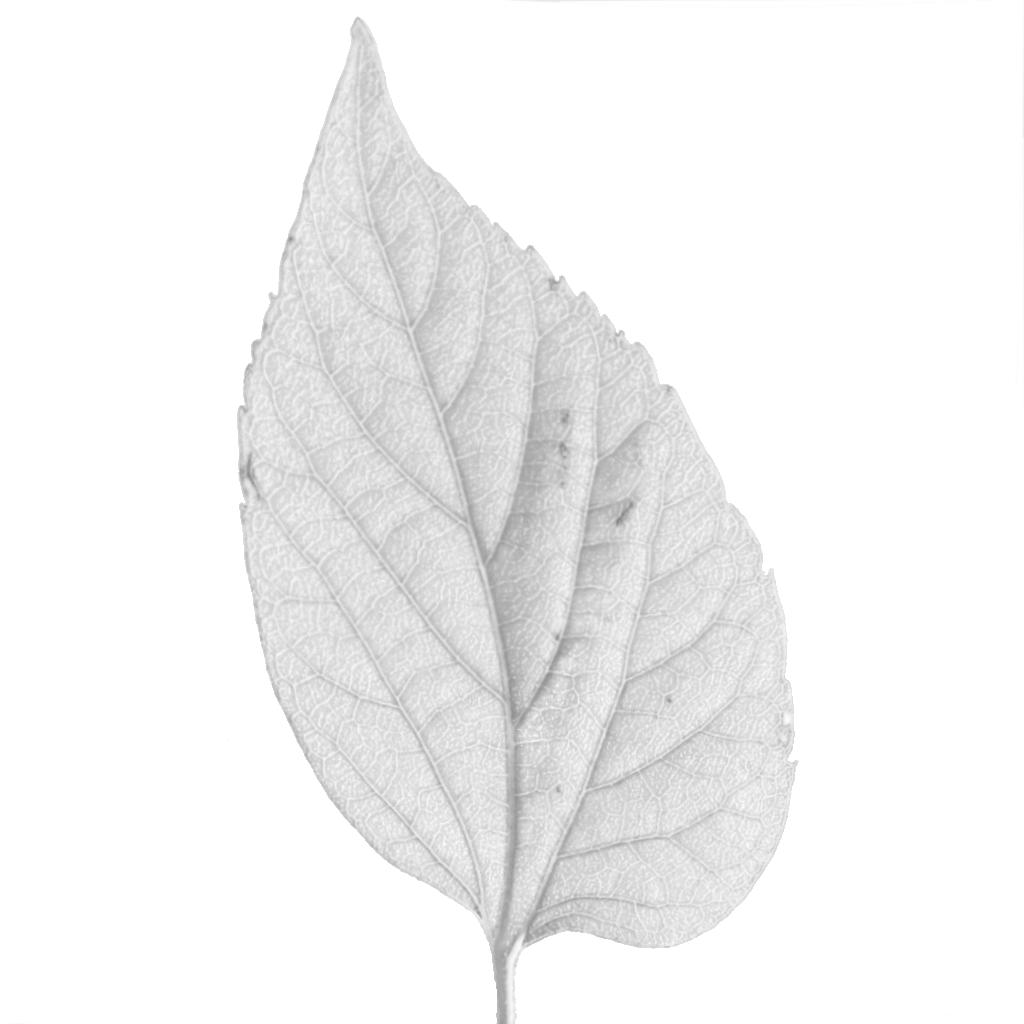
\includegraphics[width=0.2\textwidth]{./figures/leaf3_translucency_front_e.png}&
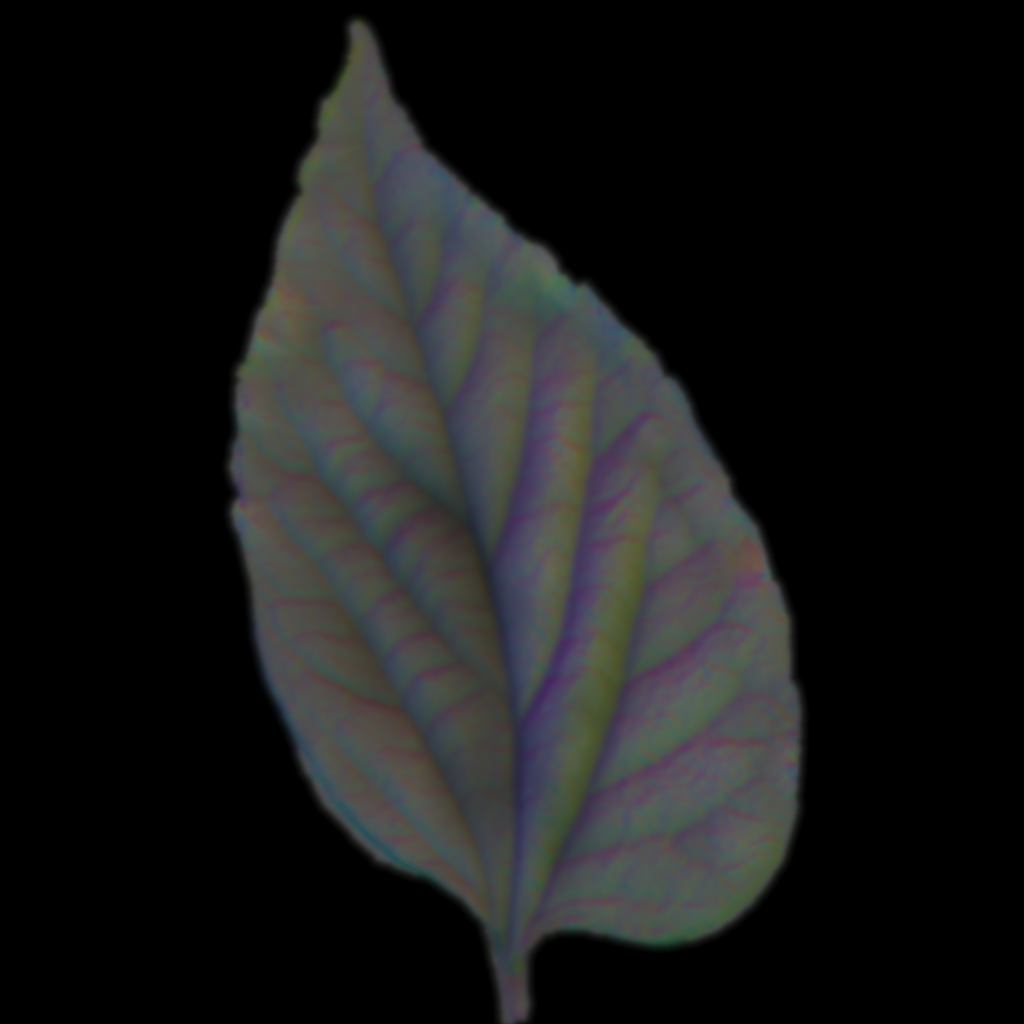
\includegraphics[width=0.2\textwidth]{./figures/leaf3_halflife2_front.png}
\\
(c)&(d)&(e)&(f)
\end{array}$
\caption[Zdrojové textury pro výpočet osvětlení listů]%
{Zdrojové textury pro výpočet osvětlení listů. (a) původní barevná mapa, (b) původní mapa průsvitnosti, (c) mapa barevných odchylek od základní barvy listu (pro názornost zvětšeny), (d) normálová mapa, (e) mapa průsvitnosti, (f) mapa koeficientů Half Life 2 bázových funkcí \label{fig:leafResources}
}
\end{figure}
Pro listy jsou ovšem k dispozici původně jiná zdrojová data. Původní barevná mapa obsahuje prosté barvy listu (např. fotografie) - jde vlastně o záznam podoby listu pro jednu sezónní barvu a tu neumožňuje přímo a jednoduše dynamicky měnit. Mapu barevných odchylek můžeme získat z původní barevné mapy odečtením základní barvy listu (později přičtena jako sezónní barva listu). Obdobné předzpracování je nutné provést s původní mapou průsvitnosti, na kterou je výhodnější nahlížet jako na mapu intenzit.  

\newpage



% LOD %%%%%%%%%%%%%%%%%%%%%%%%%%%%%%%%%%%%%%%%%%%%%%%%%%%%%%%%%
\section{Úrovně detailu}
\label{sec-LOD}
V předchozích kapitolách předpokládáme zpracování a zobrazování geometrického modelu vegetace. Pro nižší úrovně detailu (LOD) lze využít metod, které složitou geometrii typicky nahrazují zobrazením primitivní geometrie (např. čtverce), na které je aplikována textura (obrázek) navozující dojem, že se jedná o původní objekt. Zaznamenáme-li pohledy na objekt z několika směrů, lze s určitou rozumnou tolerancí ke snížení kvality zobrazit následně pomocí těchto pohledů libovolný pohled na objekt bez nutnosti zobrazení a zpracování jeho plné geometrické reprezentace. Úspora potřebného výkonu spočívá jak v malém počtu zpracovávaných vrcholů geometrie, tak v ušetření řady rasterizačních operací stejně jako v menším počtu zpracovávaných fragmentů.
\footnote{ předpokládá se, že jednotlivé listy jsou vykreslovány v náhodném pořadí a tím pádem je barva určitého pixelu několikrát přepisována}
 Výsledná kvalita zobrazeného objektu je ovlivněna počtem předgenerovaných pohledů, jejich kvalitou a také způsobem, jak zkonstruovat obraz pro pohled ze směru, pro který neexistuje předgenerovaný obraz.
Známé jsou metody billboardingu využívající pro osově souměrnou geometrii jediného pohledu, který je natáčen kolmo k pohledu virtuální kamery. \footnote{existuje několik možností natáčení obrázku např:
\begin{itemize}
\item rovnoběžně se stínítkem kamery
\item kolmo k pohledu kamery
\end{itemize}
}
Relativně běžná je metoda využívající jakýchsi trsu billboardů. Objekt je nahrazen množinou různě orientovaných geometrických primitiv, jak je patrné z obrázku 
\begin{figure}[!hbt]
\begin{center}

\includegraphics[width=0.75\textwidth]{./figures/slicesTop.png}
\caption{ Konstrukce jednoduchého trsu billboardů: (pohled zvrchu) vyšší LOD tvořený třemi skupinami billboardů po 3 řezech (vlevo), nižší LOD tvořený pouze dvěma kolmými billboardy (vpravo) }
\end{center}
\label{fig:sliceBilboard}
\end{figure}

Na rozdíl od metod skutečného billboardingu, trsy billboardů si zachovávají svou orientaci vůči světovým souřadnicím ve scéně. Tento koncept lze vylepšit pro zobrazování objektů, jako jsou stromy tím, že přidáme další rovnoběžné billboardy. Struktura koruny stromu je dosti členitá a při pohybu kolem stromu se uplatňuje paralaxa a dochází k překrývání větví a listů. K tomu dochází i v případě pohybu samotného stromu. Budeme-li uvažovat v částech průhledné obrázky použité v trsu rovnoběžných billboardů, pak lze podobných efektů docílit. Sadu rovnoběžných billboardů lze chápat jako různé řezy geometrií. Do každého řezu se promítne určité okolí tak, aby celkově všechny rovnoběžné řezy pokrývaly rovnoměrně celou původní geometrii.
\begin{figure}[!hbt]
\begin{center}
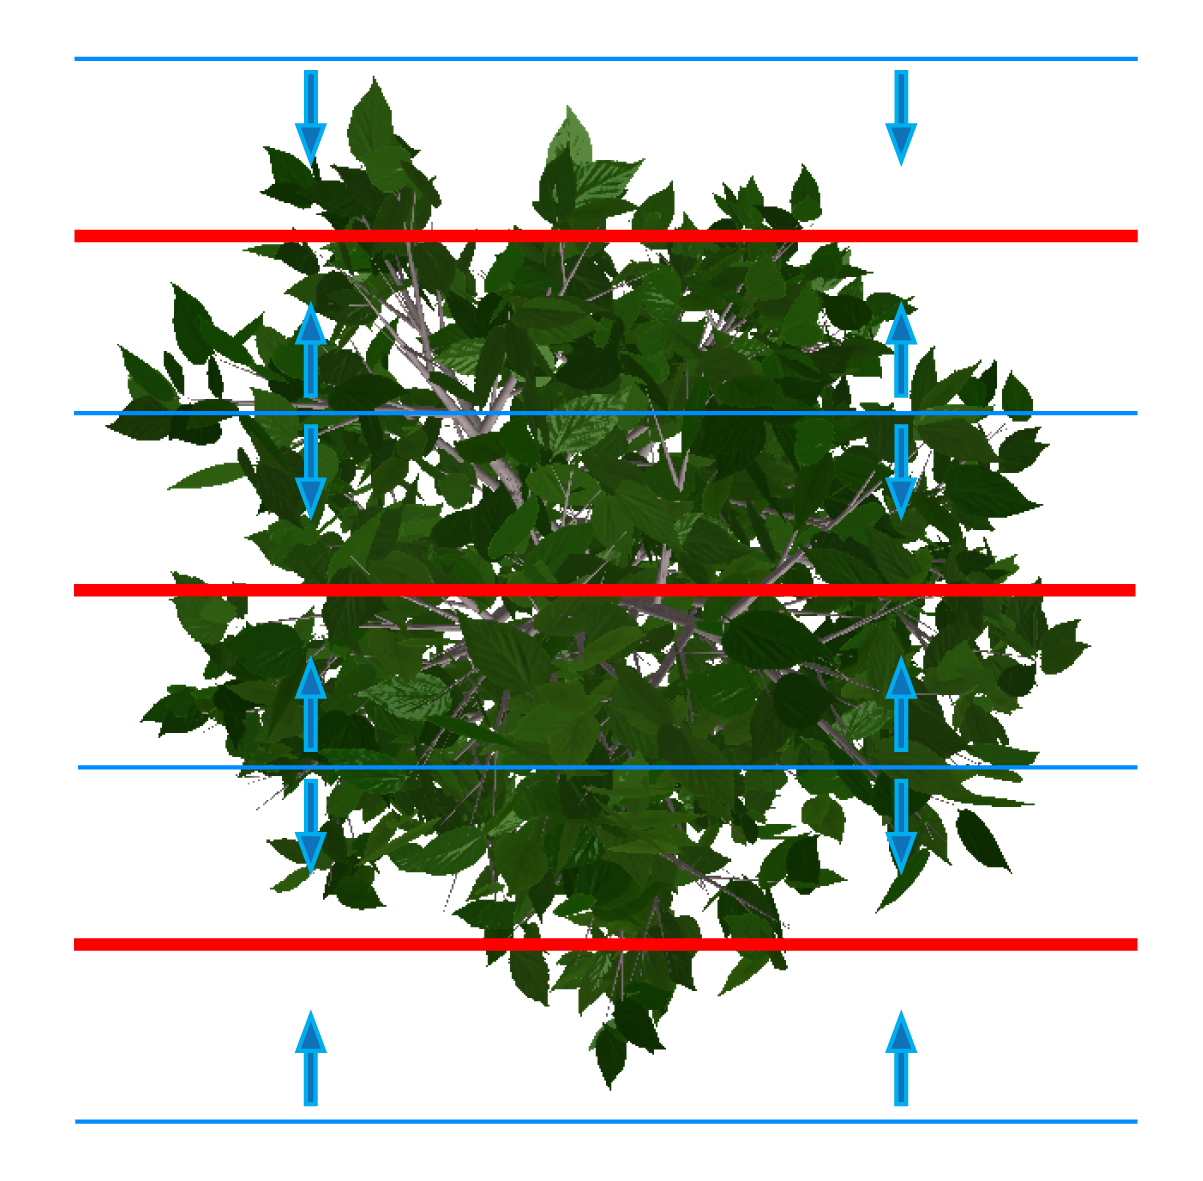
\includegraphics[width=0.5\textwidth]{./figures/slices.png}
\caption{ Tvorba řezů pro vícevrstvé billboardy. Jednotlivé textury řezů jsou znázorněny červeně. }
\end{center}
\label{fig:slicing}
\end{figure}
Čím je objekt od pozorovatele vzdálenější, tím méně se tyto efekty uplatňují a tím menší má objekt percepční váhu, proto lze v rámci zvýšení výkonu snižovat počet obrázků (textur) v trsu.
Protože se orientace trsu řezů vůči scéně nemění, mohou vznikat nepříjemné artefakty tím, že směr pohledu bude téměř rovnoběžný s rovinou některého z řezů. Z toho důvodu je dobré zajistit, aby se takové řezy vůbec nezobrazovaly.
Řezy lze předgenerovat pro statický strom a používat je následně pro každou instanci daného stromu ve scéně.


\subsection{Animace v image-base modelu}
\label{sec-ibAnimation}

Bohužel z povahy konstrukce trsu řezů dochází ke ztrátě velikého množství informací, které jsou podstatné pro provedení animace v rozsahu a kvalitě odpovídající postupu popsaného v kapitole Animace trojrozměrného modelu. Větve jsou například většinou zakryty listy. Jednotlivé listy se také překrývají a tak například o listech, které nejsou vidět nelze získat žádné informace. Naštěstí nemají modely zobrazené touto metodou vysokou percepční váhu (jde o nižší LOD) a lze si tudíž dovolit snížení kvality a přistoupit k animaci zcela jinak.
Základním předpokladem je, že deformace se provádí pouze v dvourozměrném prostoru textury jednoho řezu. Zatímco původní deformace je realizovatelná ve vertex shaderu, tento postup využije s výhodou možností fragment shaderu. Vyplývá z toho však nepříjemné omezení, které mění původní problém, který lze shrnout otázkou: \emph{„Kam se posune tento bod?“} (nazývejme {\bf přímá transformace}), na problém typu \emph{„Jaký bod se přesune do tohoto místa?“} (nazývejme {\bf zpětná transformace}). Fragment shader totiž neumožňuje měnit aktuálně zpracovávanému fragmentu pozici, na kterou bude zapsán ve výstupním bufferu. Uvážíme-li, že se na určitou pozici může po transformaci zobrazit i několik fragmentů, bylo by pro korektní zobrazení nutné projít každý texel textury provést přímou transformaci a zjistit, zda není dosaženo aktuální pozice. Takové řešení je ovšem značně nevhodné.

Jestliže je třeba provádět v rámci jediné textury různé transformace, které přísluší různým zobrazeným větvím, pak je třeba znát, jaká transformace se v daném bodě bude provádět. Musí být tedy předem jasné, jaká větev se do daného bodu může zobrazit. Současně s generováním textur pro jednotlivé řezy, je možné připravit i texturu, která bude tuto informaci obsahovat. Jednoduchým řešením, které lze i efektivně implementovat na GPU, je vytvoření oblastí, které odpovídají buňkám Voronoiova diagramu – tedy pro daný bod nalezneme nejbližší bod, kde je zobrazena větev ve výchozím stavu. Tento postup můžeme nazvat {\bf „propagace dat“}.

\begin{figure}[!hbt]
\label{fig:sliceBilboard}
\begin{center}
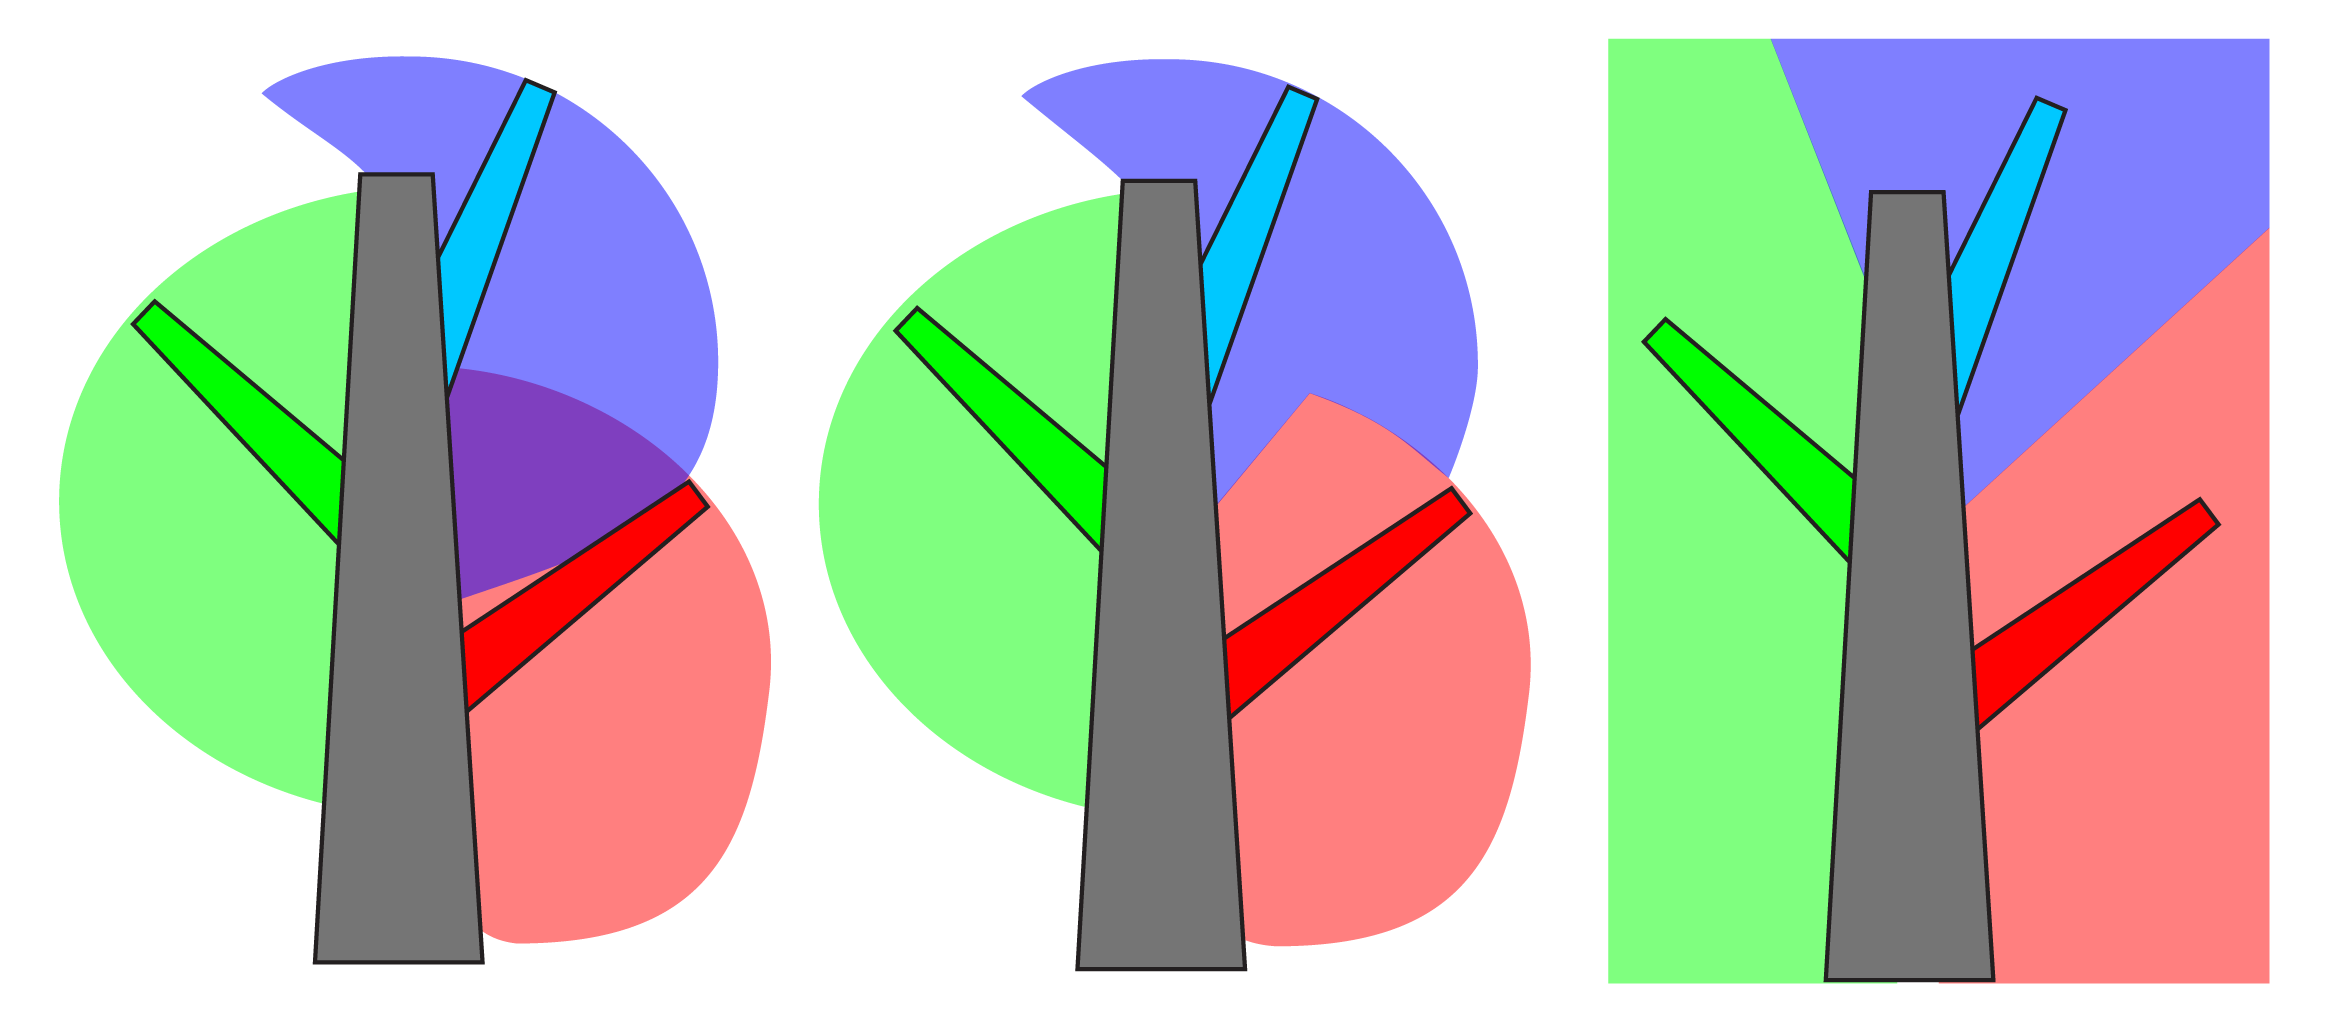
\includegraphics[width=0.75\textwidth]{./figures/dataExpansionPrinciple.png}
\caption[Schematicky znázorněné oblasti, kam se mohou větve deformovat]%
{Schematicky znázorněné oblasti, kam se mohou větve deformovat. Černě vytaženy obrysy výchozí polohy zobrazených větví
(vlevo) reálný ohyb – oblasti se překrývají, (uprostřed) oblasti bez překryvů, (vpravo) oblasti Voronoiova diagramu}
\end{center}
\end{figure}

Pokud tedy známe, jaká větev se může do daného bodu $P$ deformovat, známe také parametry této deformace. Z důvodů zachování koherence animace (větve se pohybují zhruba stejně) využijeme metodu deformace vycházející z ohybu trojrozměrného modelu. Trojrozměrný ohyb je prováděn v souřadném systému větve ($S_b$). Po převedení bázových vektorů ($\vec{r}_b$,$\vec{s}_b$,$\vec{t}_b$) do souřadného systému řezu ($S_p$ – tedy vektory $\vec{r}_p$,$\vec{s}_p$,$\vec{t}_p$) je možné postupovat prakticky stejně. Uplatníme myšlenkový model, kdy bod $P_0$ mimo větev (představovaná osou x) bude při deformaci udržovat svou relativní pozici na normále k větvi (viz obrázek \ref{fig:bendModel}). Potřebujeme tedy zjistit, ke kterému bodu větve je bod $P_p$ ukotven.

\begin{figure}[!hbt]
\begin{center}
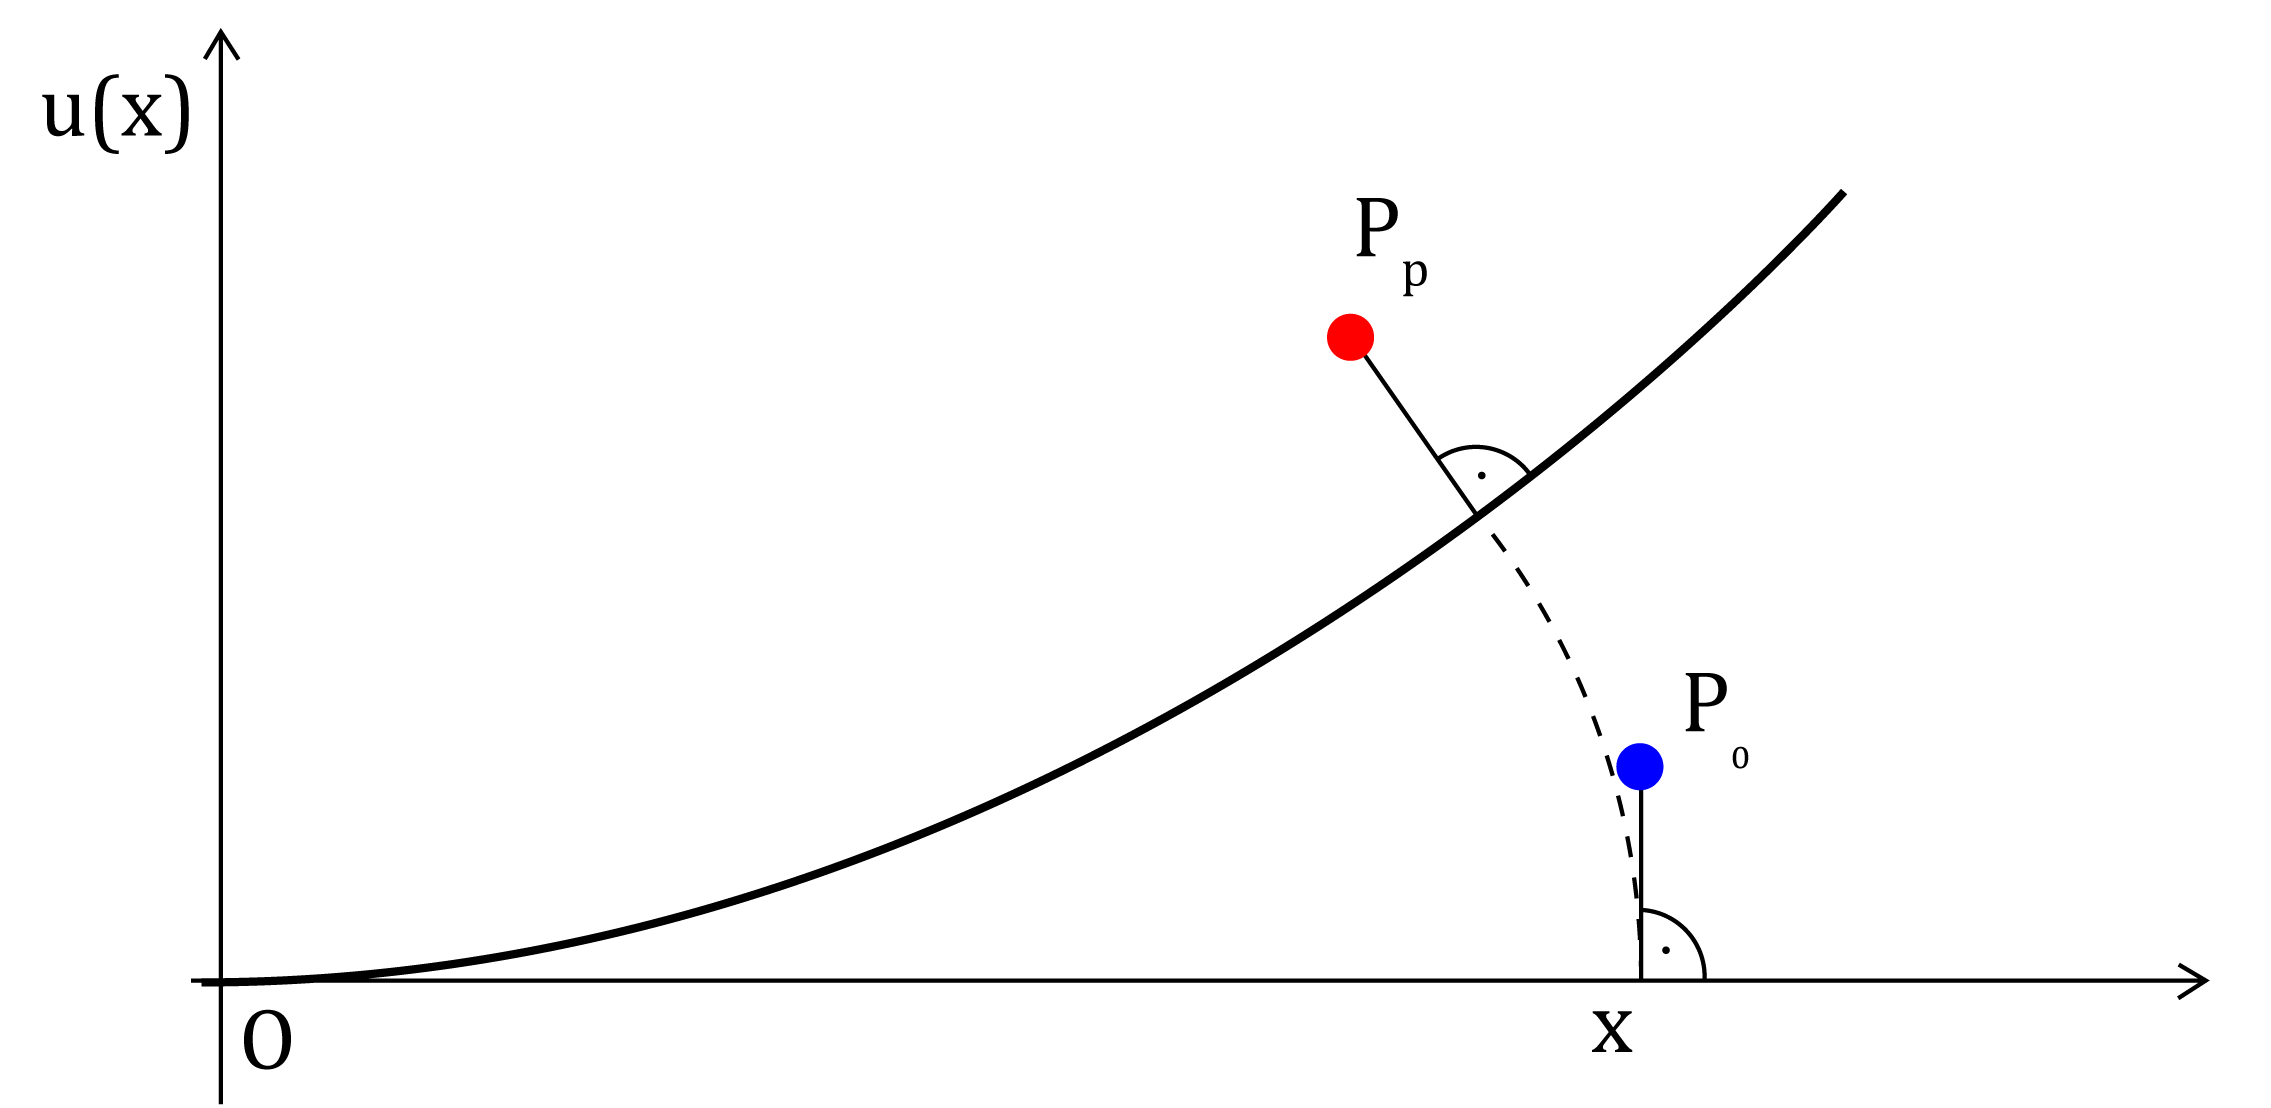
\includegraphics[width=0.5\textwidth]{./figures/revDef_ideal.png}
\caption{Myšlenkový model ohybu pomocí zpětné transformace\label{fig:bendModel}}
\end{center}
\end{figure}
 
Problém představuje určení parametru $x$ ohybové funkce $u(x)$ pro bod $P_p$ (deformovaný z $P_0$), který zmíněnou polohu na větvi definuje. Pro přesné určení je nutné zjistit nejbližší bod na ohybové funkci a pro ten pak zjistit jeho vzdálenost na křivce od počátku. 
\begin{figure}[!hbt]
\begin{center}
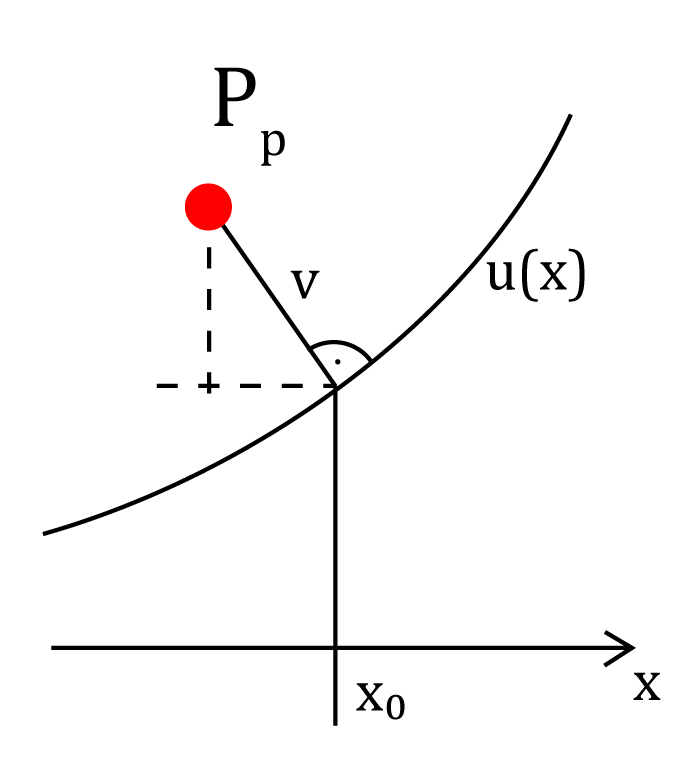
\includegraphics[width=0.25\textwidth]{./figures/revDef_dist.png}
\caption{Zjišťování nejbližšího bodu na ohybové křivce $u(x)$\label{fig:closestPointOnCurve}}
\end{center}
\end{figure}

Bod $x_0$ lze určit z následujících rovnic, kde hledáme minimum pro vzdálenost $v$:

\begin{align}
\frac{\mathrm {d}{v}}{\mathrm {d}{x_0}} &= 0 \nonumber\\
v &= \sqrt{(x_0 - P_{px})^2 + (u(x_0) - P_{py})^2} \nonumber\\
\frac{\mathrm {d} \sqrt{(x_0 - P_{px})^2 + (c_2x_0^2 +c_4x_0^4 - P_{py})^2}}{\mathrm{d}x_0} &=0
\end{align}
Řešení je omezeno podmínkou:
\begin{align}
P_{px} \neq \pm \sqrt {\frac{-c_2 \pm \sqrt{c_2^2 - 4c_4P_{py}}}{2c_4}}
\end{align}

a transformuje se na problém hledání kořenů polynomu 7. stupně:

\begin{align}
\label{closestPointEq}
4c_4^2 x^7 + 6c_2c_4x^5 + (2c_2^2 - 4P_{py}c_4)x^3 + (1-2P_{py}c_2)x - P_{px} &= 0
\end{align}

Tento polynom nemá triviální řešení a může se stát, že řešení je i několik – což odpovídá situaci, kdy se více bodů z křivky deformuje do stejného místa (viz obrázek ~\ref{fig:multisolution} ).
\begin{figure}[!hbt]
\begin{center}
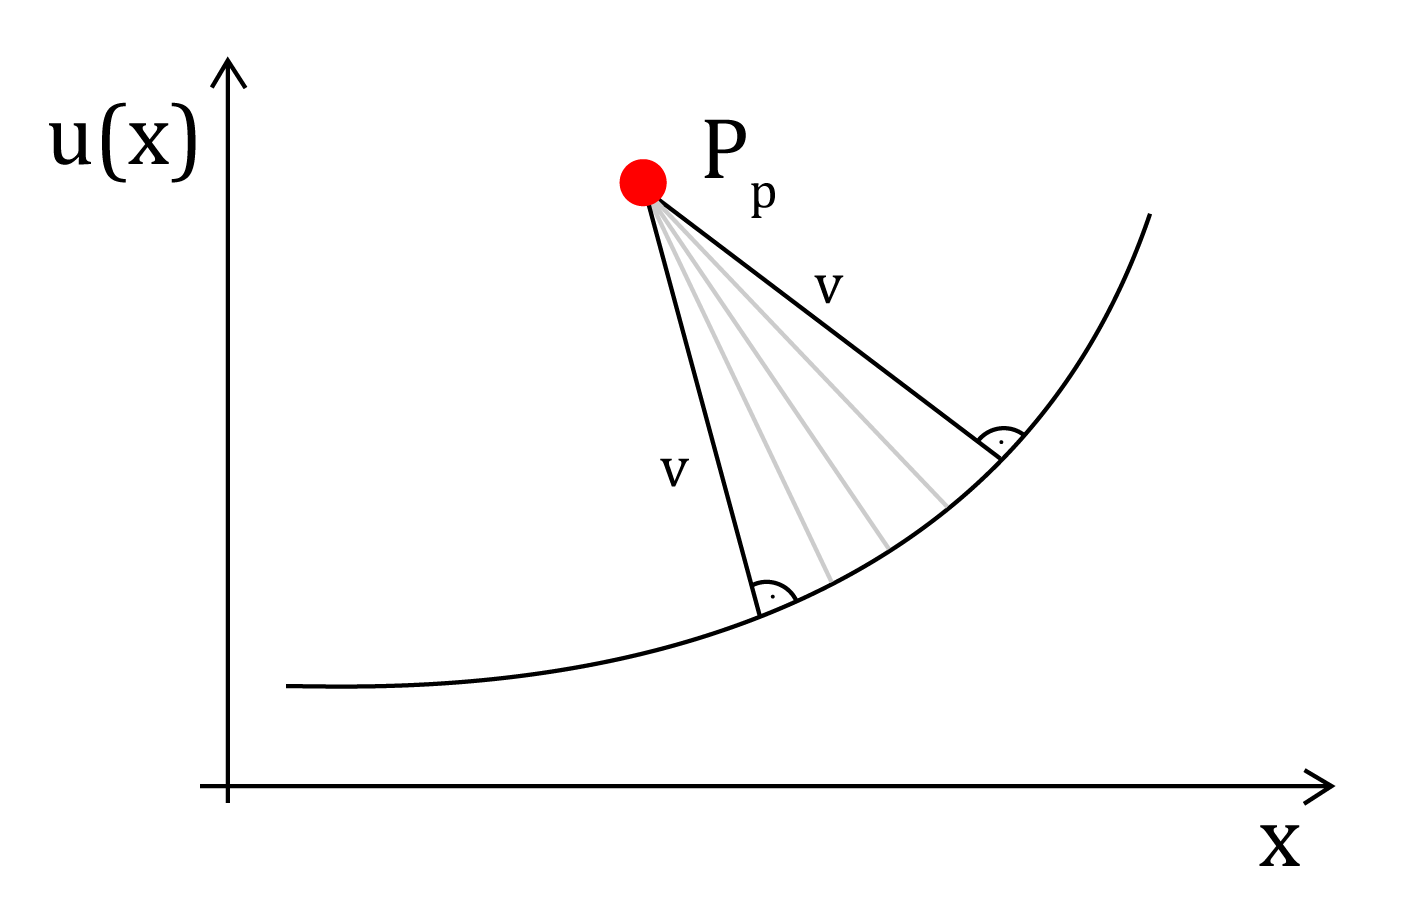
\includegraphics[width=0.5\textwidth]{./figures/revDef_multisolution.png}
\caption[Mnohoznačnost při zpětné transformaci]
{Znázornění problému mnohoznačnosti při určování, který bod je řídící pro zpětnou deformaci bodu $P_p$. U reálného stromu dojde v tomto případě ke kolizi takových větví.\label{fig:multisolution}}
\end{center}
\end{figure}

Krom obtíží s řešením kořenů polynomu \eqref{closestPointEq} se tak přidává i určitá nejednoznačnost. Stále je však ještě potřeba vyřešit vzdálenost takto nalezeného bodu na ohybové křivce. Uvážíme-li, že takový složitý postup by se měl provádět pro každý zobrazovaný fragment textury, dostaneme se do patové situace.
Zde je třeba rezignovat na dodržení shodného postupu jako v případě přímé deformace geometrie. Počáteční bod $O$ příslušné větve převedeme do souřadného systému textury ${S_p}$ a zjistíme projektovanou délku $L$ větve. {\bf Hledanou hodnotu x pak nahradíme vzdáleností $\left| OP \right|$, kterou normujeme délkou $L $ a omezíme na rozsah $\left \langle 0;1 \right \rangle$ }. Pro takovou hodnotu $x$ určíme deformační vektor $\vec{d}$ (posunutí bodu) a aplikujeme v opačném směru $\vec{-d}$ než při přímé transformaci.
 
\begin{figure}[!hbt]
\begin{center}
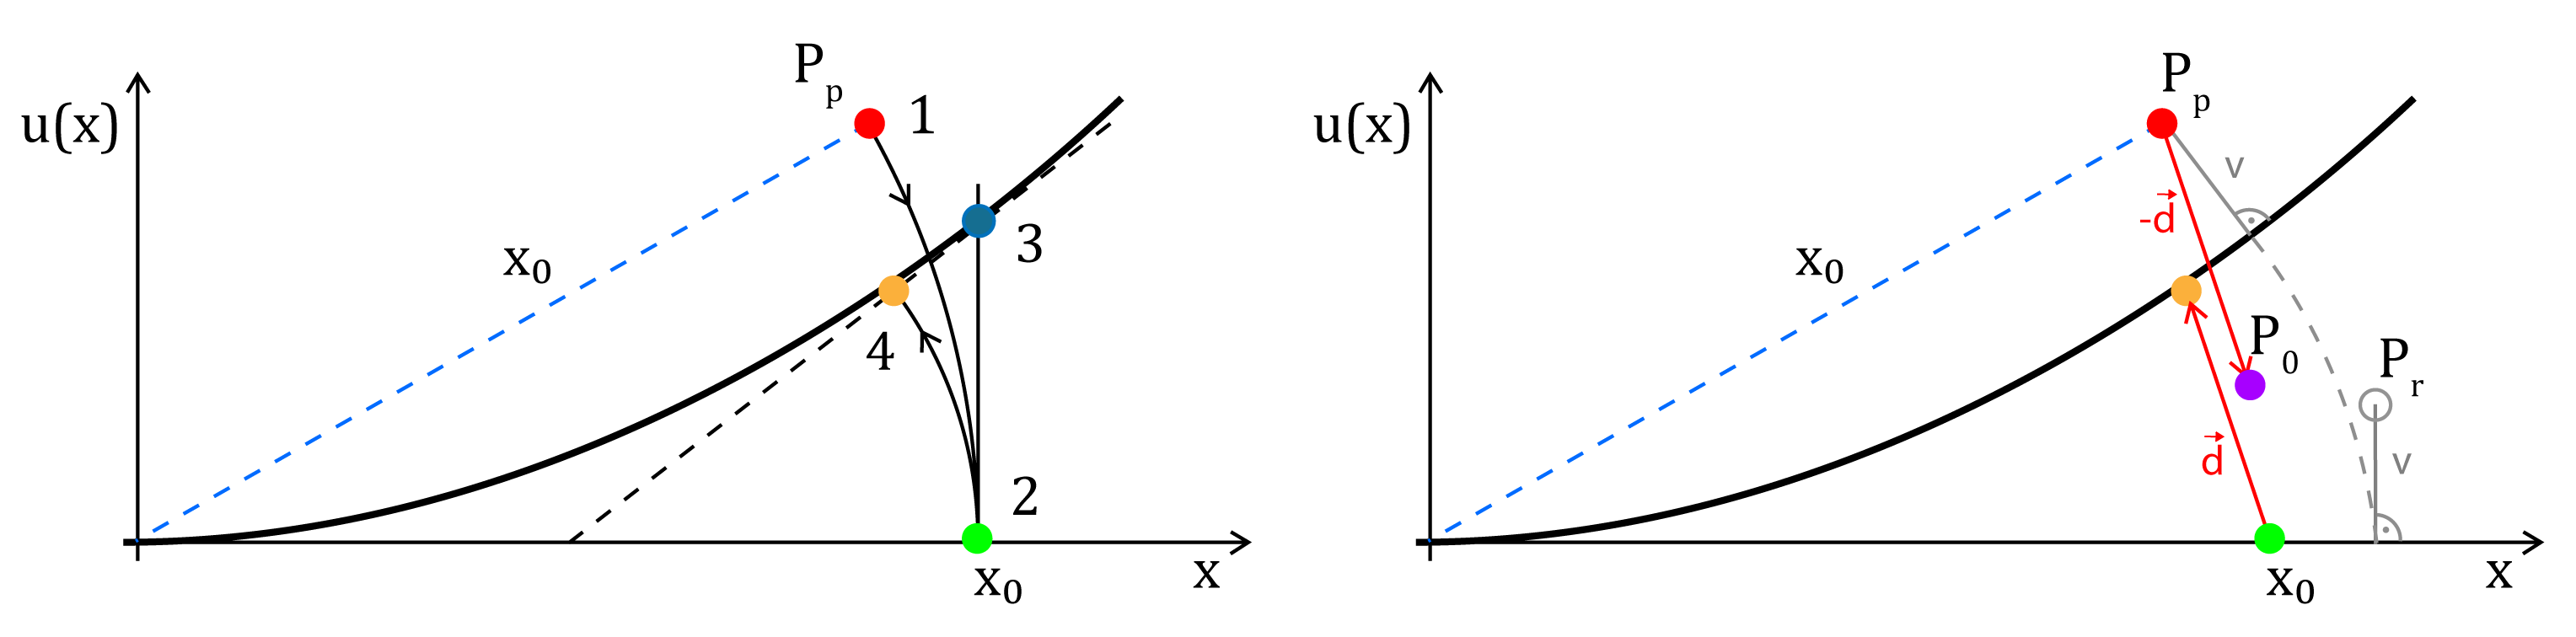
\includegraphics[width=1.0\textwidth]{./figures/revDef_process.png}
\caption[Postup zpětné transformace]
{Postup zpětné transformace: (vlevo) – postup určení deformace: Bod $P_p$ (1), pro který určujeme deformaci je ve vzdálenosti $x_0$ od počátku (2). Zjistíme hodnotu ohybové funkce v bodě $x_0$ (3). Provedeme korekci délky (4).
(vpravo) – určíme vektor posunutí $\vec{d}$ mezi body $x_0$ a (4) (v obrázku vlevo) odečtením od bodu $P_p$ se dostáváme na pozici předobrazu $P_0$. Šedivě je naznačen bod $P_r$, jež je skutečným předobrazem respektujeme-li myšlenkový model. \label{fig:backwardTransformationProcess}}
\end{center}
\end{figure}
\pagebreak
Je patrné, že chyba způsobená takovou hrubou aproximací $x_0$ je relativně malá pro body $P_p$, ležící přímo na ohybové křivce, ale roste tím víc, čím je od ní bod vzdálenější. Použitím vztahů \eqref{lengthCorrection} aplikovaným na projektované bázové vektory $\vec{r}_p$, $\vec{s}_p$ (zastoupené vektorem $\vec{b}_p$) dostaneme upravené vztahy pro korekce délky $\vec{c}_{\vec{b}}$, $\vec{c}_{\vec{b}}$.

\begin{align} 
\vec{c}_{\vec{b} }&= \vec{t} + \vec{b} \cdot f'_{\vec{b} } (x)\cdot\frac {d_{\vec{b} }(x)}{s_{\vec{b} }(x)}
 \end{align}

Deformaci v prostoru textury lze tedy popsat následovně:

\begin{align}
\label{backwardDeformation} 
\vec{P}_0 &= \vec{P}_p - \left ( u_{\vec{r}} (x) \cdot \vec{r}_p + u_{\vec{s}} (x) \cdot \vec{s}_p - \left (\vec{c}_{\vec{r}} +\vec{c}_{\vec{s}}  \right ) \right )
\end{align}


Zpětnou deformaci lze provádět i hierarchicky a to v pořadí od nejnižší úrovně větví v hierarchii až po kmen (tedy opačně, než v přímé transformaci). Je však nutné vyvážit náročnost takového postupu a jeho přidanou hodnotu. Například je možné deformaci provádět pro několik nejvyšších úrovní hierarchie. 
S opačným postupem tvorby hierarchické deformace v image-based modelu souvisí i problém správné aplikace směrové složky větru. Ve vztahu \eqref{windEq} je použit vektor $\vec{t}$ ovlivněný nadřazenými deformacemi. Ten však při opačném postupu zpětné deformace není znám. Předpokládáme-li provádění zpětné deformace pouze ve dvou úrovních (kmen + větve první úrovně) a rozumě malé výchylky, pak lze za vektor $\vec{t}$ dosadit nedeformovaný vektor $\vec{t}_p$, místo $\vec{W}$ použijeme $\vec{W}_p$ (směr větru v souřadné soustavě řezu). Vzniklá chyba není natolik vážná, aby představovala překážku u modelů s nižší percepční vahou, jakými nižší stupně LOD bezpochyby jsou.

Popsaná metoda má předpoklad dobře fungovat pro větve tvořící siluetu stromu v daném řezu. U takových větví se předpokládá, že jejich podélný vektor je zhruba rovnoběžný s rovinou řezu. Současně je třeba si uvědomit, že i fáze propagace dat má určitá omezení a funguje lépe pro siluetové větve. Jak se však ukazuje, právě tyto větve hrají největší roli při pozorování stromu s nižší percepční vahou. Hrají i podstatnou roli při přechodu mezi úrovněmi LOD.

Zbývá vyřešit pohyb jednotlivých listů. Pohybem větví nižších úrovní hierarchie a listů vzniká vysokofrekvenční šum v prostoru obrazu. Tento šum pozorovatel vnímá, ale nerozeznává již, jestli je způsoben pohybem větví, či samotných listů. Lze ho tedy napodobit použitím jediné deformace. Pro šum vyšších frekvencí je zároveň těžké rozlišit, zda jde čistě o pohyb, či jen změny barvy. Představíme-li si například, že list je zobrazen do jediného pixelu, pak pouhým natáčením listu zjevně měníme barvu zmíněného pixelu (barevný šum). Nerotační pohyb listu může způsobit obarvení jiného pixelu (pohybový šum). Pohyb listů může pak ústit v určité nepravidelné chvění elementárních fragmentů obrazu (případně větších oblastí – podle toho, kolik fragmentů zobrazuje stejný list).
Pohybovou složku šumu lze vcelku dobře napodobit metodou zvanou {\bf displacement-mapping}. V základní verzi získává z řídící textury informace o posunutí v prostoru deformovaného obrazu – v tomto případě barevné textury. Vhodnými změnami řídící textury (posun souřadnic, kombinace různých textur) lze plynule deformovat výsledný obraz. 
\begin{figure}[!hbt]
\begin{center}
$\begin{array}{cc}

\includegraphics[width=0.35\textwidth]{./figures/distortion_before.png}&

\includegraphics[width=0.35\textwidth]{./figures/distortion_after.png}
\end{array}$
\caption[Postup zpětné transformace]
{Postup zpětné transformace: (vlevo) – postup určení deformace: Bod $P_p$ (1), pro který určujeme deformaci je ve vzdálenosti $x_0$ od počátku (2). Zjistíme hodnotu ohybové funkce v bodě $x_0$ (3). Provedeme korekci délky (4).
(vpravo) – určíme vektor posunutí $\vec{d}$ mezi body $x_0$ a (4) (v obrázku vlevo) odečtením od bodu $P_p$ se dostáváme na pozici předobrazu $P_0$. Šedivě je naznačen bod $P_r$, jež je skutečným předobrazem respektujeme-li myšlenkový model. \label{fig:backwardTransformationProcess}}
\end{center}
\end{figure}


Šumový displacement-mapping je možné zapsat například takto:

\begin{align} 
color &= T_{color}(T_{def}(\vec{o}_t + t \cdot \vec{d}_1)+T_{def}(\vec{o}_t + t \cdot \vec{d}_2)),
\end{align}
kde $T_{def}(\vec{x})$ je texturovací funkce, jež zobrazuje souřadnice $\vec{x}$ na jiné, a $T_{color}(\vec{x})$ přiřazuje daným souřadnicím $\vec{x}$ barvu. 
Barevnou složku šumu je možné vytvořit například tak, že pro každý zobrazený list v řezu měníme jeho natočení ke světlu (normálu) a následně provádíme standardní vyhodnocení Phongova osvětlovacího modelu.

\pagebreak
\subsection{Řízení úrovně detailu}
\label{sec-LODcontrol}
V předchozích kapitolách jsou navrženy metody, jak zobrazovat vegetaci (stromy) ve třech různých stupních detailu. Nejvyšší (označme ji \emph{LOD\_0}) využívá podrobné geometrické reprezentace a poskytuje nejlepší kvalitu zobrazení pro pohledy zblízka. Přesvědčivě tak lze zobrazit i jednotlivé pohybující se listy stromu. LOD\_0 je však vcelku náročná na výkon a není možné ji uplatnit plošně na všechny stromy rozsáhlé lesní scény. Pro stromy s nižší percepční vahou (není třeba je zobrazovat tak podrobně) byly navrženy image-based metody (označme LOD\_1 a LOD\_2). Ty poskytují sice nižší kvalitu zobrazení (na úrovni zobrazení a pohybu celého stromu), ale jsou méně náročné na výkon. 
\begin{figure}[!hbt]
\begin{center}
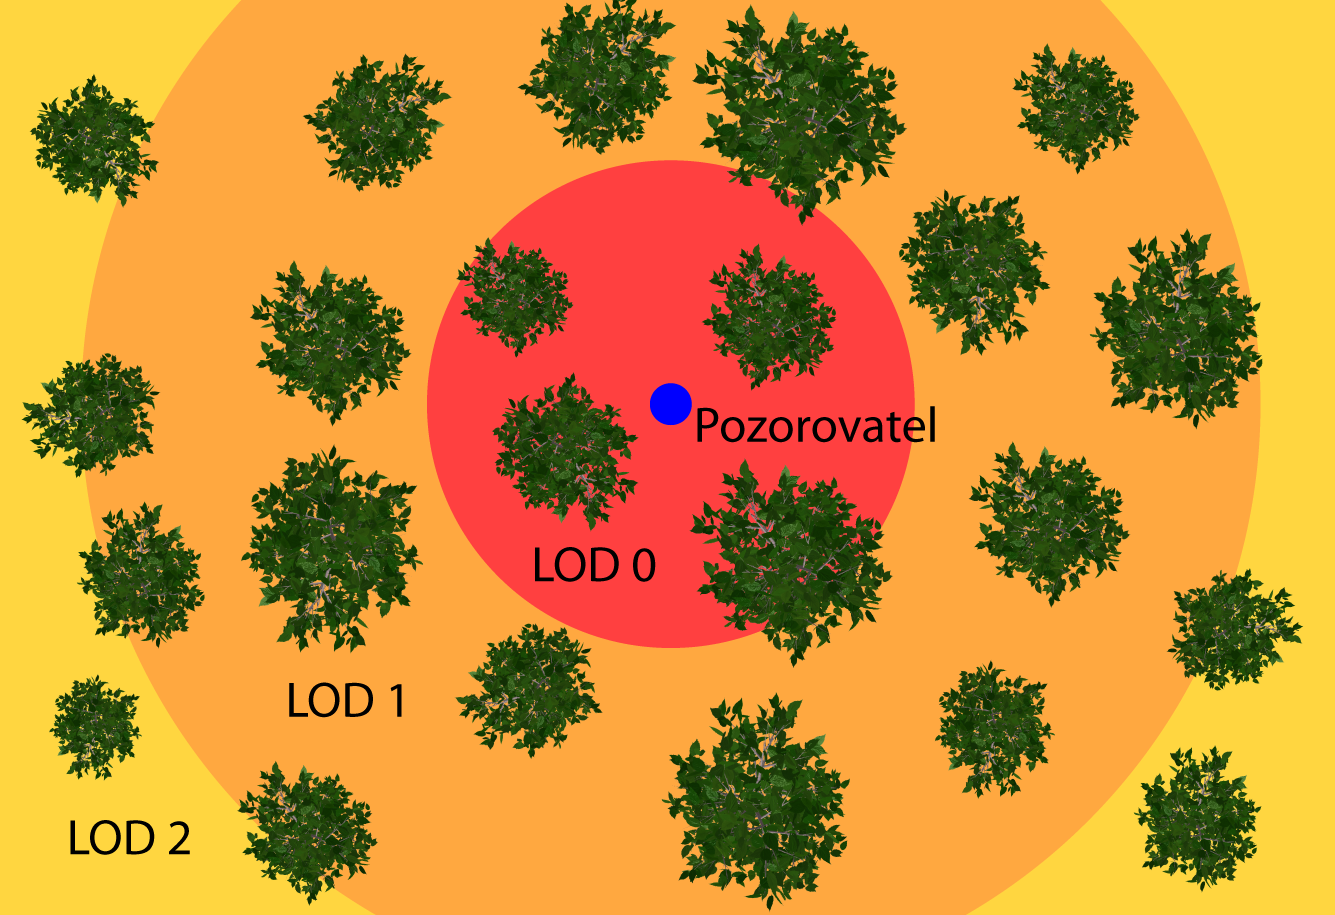
\includegraphics[width=0.75\textwidth]{./figures/LODcontrol.png}
\caption{Znázornění zón, kde se instance stromů vykreslují danou metodou.\label{fig:lodZones}}
\end{center}
\end{figure}

Pro určení přibližné percepční váhy se běžně využívá vzdálenostní kritérium. Blízké stromy v okolí pozorovatele jsou tedy zobrazeny metodou LOD\_0, od určité vzdálenosti $v_1$ se využívá metody LOD\_1 a obdobně pro vzdálenost $v_2$ a metodu LOD\_2, přičemž platí, že $0<v_1<v_2$ .

Jedná se tedy o diskrétní třístupňový LOD systém. Určení vzdálenosti k jednotlivým instancím stromu lze provádět buď v prostoru (vhodné např. aplikace typu letecký simulátor), nebo pouze v horizontální rovině (aplikace s pohledem omezeným na pohled z okolí úrovně terénu). Vzdálenosti $v_1$ a $v_2$ je třeba přizpůsobit konkrétním modelům vegetace a scéně obecně, stejně jako optimalizaci z hlediska výkonu, na který mají podstatný vliv.


\subsection{Přechody mezi úrovněmi detailu}
\label{sec-LODtransitions}

%Analýza a návrh implementace (včetně diskuse různých alternativ a volby implementačního prostředí).


%*****************************************************************************
\chapter{Realizace}
\label{chap:realizace}

V předchozí kapitole byly teoreticky rozebrány nejpodstatnější a nejdůležitější části práce. Ovšem i tak zbývá řada problémů, které je nutné v rámci realizace dořešit. 

% obrázek finálního "renderu"
\begin{figure}[here]
\begin{center}
$\begin{array}{cc}
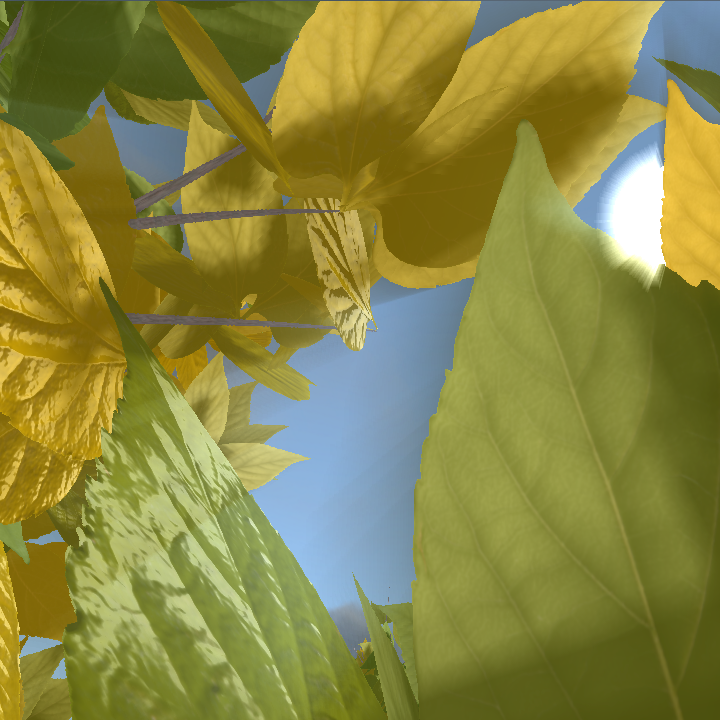
\includegraphics[width=0.45\textwidth]{./figures/final-leaves_H.png}&
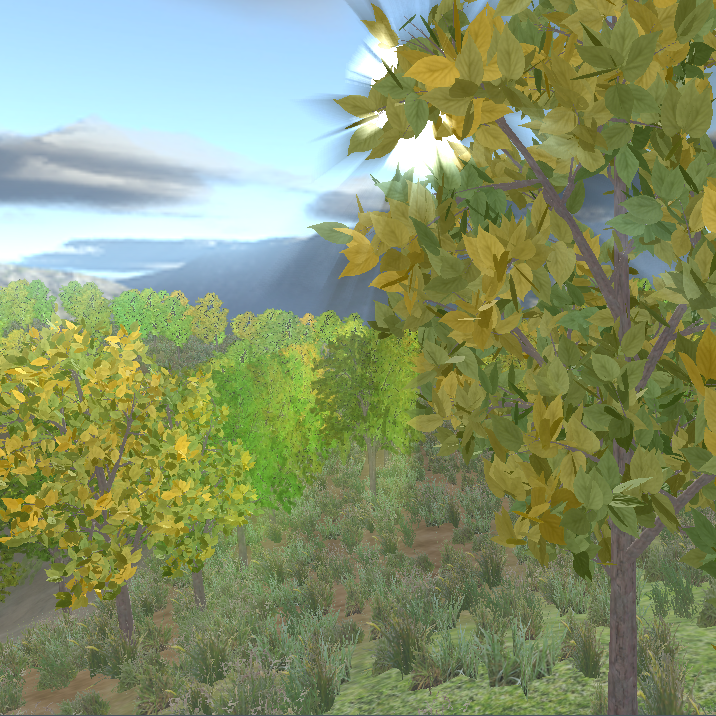
\includegraphics[width=0.45\textwidth]{./figures/final-trees_H.png}\\
(a)&(b)\\
\end{array}$
\caption[Ukázka výsledného zobrazení]%
{Výsledné zobrazení. Detail listů (a), kde je patrná průsvitnost i lesklost. Rozsáhlejší scéna s více stromy (b).\label{fig:resultA}
}
\end{center}
\end{figure}
V následujícím textu bude stručně popsáno, jejich řešení. Budou zmíněny technologie a knihovny, které byly pro realizaci použity, a popsána vstupní data výsledného programu, jejich zpracování a použití. Opomenuta nezůstane ani celková architektura systému a konkrétní řešení zobrazování všech úrovní detailu (LOD).

\pagebreak

%%%%%%%%%%%%%%%%%%%%%%%%%%%%%%%%%%%%%%%%%
\section{Použité technologie, frameworky a knihovny}
\label{sec-frameworks}

Výsledná aplikace byla implementována v jazyce {\bf C/C++} a využívá knihovnu {\bf OpenGL} \cite{openGL}. Ta poskytuje efektivní aparát pro práci s grafickým hardware a umožňuje využít většiny jeho nejnovějších vlastností a funkcí. Její výhodou je platformová nezávislost. Stejný kód by tedy mělo být možné přeložit jak pro Windows, tak pro systémy Unixového typu. Následně bylo využito několika dalších knihoven zjednodušujících práci se základní OpenGL:
\begin{description}
\item[GLFW] \cite{GLFW} sada knihovních funkcí určených pro snadné vytváření oken, OpenGL kontextů a mapování vstupních zařízení. Zachovává platformní nezávislost a uplatňuje se zejména ve fázi inicializace aplikace. Pomocí této knihovny je vytvořeno okno potřebných vlastností (podporuje i multisampling).
\item[GLUT] \cite{GLUT} sada nástrojů pro efektivnější práci. Obsahuje funkce pro vytváření oken a kontextů, mapování vstupů i pro práci s grafickými prvky.
\item[GLEW] \cite{GLEW} knihovna pro práci s rozšířeními (extenzemi) OpenGL. Zahrnuje zejména funkce pro zjišťování, zda ovladač grafického hardware danou extenzi podporuje.
\end{description}
Další knihovnou, která byla využita, je {\bf LODEpng} \cite{LODEpng}. Jde o jednoduchý dekodér a enkodér obrazového formátu PNG, který je distribuován formou jednoho \emph{.cpp} a jednoho {.h} souboru. Je s výhodou využit pro načítání obrázků do textur.

% obrázky zákl. ovládacích prvků
\begin{figure}[!hbt]
\begin{center}
$\begin{array}{cc}
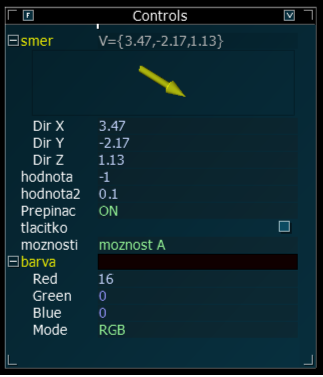
\includegraphics[width=0.35\textwidth]{./figures/ATWgui.png}&
\includegraphics[width=0.3\textwidth]{./figures/ATWgui3.png}\\
(a)&(b)\\
\end{array}$
\caption[AntTweakBar, jednoduché GUI]%
{AntTweakBar, (a) ukázka základních ovládacích prvků (shora): ovladač směru, celočíselná skalární hodnota, desetinná skalární hodnota, dvoustavový přepínač, tlačítko, seznam možností, výběr barvy.  (b) různé způsoby zadávání hodnot (shora): přímé zadání, zadání pomocí tzv. RotoSlideru, pomocí krokovacích tlačítek \label{fig:ATWgui}
}
\end{center}
\end{figure}
Pro snadnou tvorbu grafického uživatelského rozhraní (dále jen GUI) byla využita knihovna {\bf AntTweakBar} \cite{AntTweakBar}. Ta umožňuje jednoduchou tvorbu grafických ovládacích prvků, které se nejčastěji používají při práci s 3D grafickou aplikací (viz obr. \ref{fig:ATWgui}). Těmito ovládacími prvky pak lze snadno bezprostředně a přímo ovlivňovat chování zobrazované scény - v tomto případě stromů.







%%%%%%%%%%%%%%%%%%%%%%%%%%%%%%%%%%%%%%%%%
\section{Vstupní data a předzpracování}
\label{sec-modelAnalysis}
Aplikace načítá celou řadu dat, se kterými dále pracuje. V první řadě je nutné načíst popis stromu, dále pak textury použité pro jeho zobrazení. Načtená data je v řadě případů nutno předzpracovat, aby je bylo možné využít. Právě popisem vstupních dat a jejich předzpracováním se bude zabývat následující text.

%%%%%%%%%%%%%%%%%%%%%%%%%%%%%%%%%%%%%%%%%%%
\subsection{Formát OBJT}
Jelikož běžné modely stromů neobsahují implicitně informace o topologii stromu, která je nezbytná pro provedení animace, byl navržen formát vstupního souboru OBJT, který zahrnuje právě tyto informace. Soubor formátu OBJT je vstupním souborem popisujícím model stromu. OBJT je textový formát obsahující 4 druhy záznamů (oddělených standardním oddělovačem řádků):
\begin{itemize}
\item pojmenování stromu na začátku souboru entitou \lineCode{name = "\%sting\%"}
\item entita popisující větev \begin{verbatimtab}
B  %int% { 			// identifikátor větve
  l   	%int%			// úroveň v hierarchii
  d 	%float%			// délka větve
  z  	%float%	%float%	%float%	// pozice začátku větve
  k 	%float%	%float%	%float%	// pozice konce větve
  r  	%float%	%float%	%float%	// bázový vektor r
  s  	%float%	%float%	%float%	// bázový vektor s
  t  	%float%	%float%	%float%	// bázový vektor t (podélný)
  p  	%int%			// identifikátor rodičovské větve
  x  	%float%	// v kolikátině rodičovské větve se větev odpojuje
}
\end{verbatimtab}
\item entita popisující list  \begin{verbatimtab}
L  %int% { 			// identifikátor listu
  r  	%float%	%float%	%float%	// bázový vektor r
  s  	%float%	%float%	%float%	// bázový vektor s
  t  	%float%	%float%	%float%	// bázový vektor t (podélný)
  p  	%int%			// identifikátor rodičovské větve
  x  	%float%	// v kolikátině rodičovské větve se list odpojuje
}
\end{verbatimtab}
\item řádkový komentář začínající \lineCode{// \%string\%}
\end{itemize}

Ve výše uvedeném popisu formátu jsou použity zástupné řetězce za celá čísla (\lineCode{\%int\%}), za desetinná čísla (\lineCode{\%float\%}) a za znakové řetězce bez oddělovače konce řádků (\lineCode{\%string\%}). Všechny souřadnice se předpokládají v souřadném systému celého stromu (též \emph{object space}).

Data ze zdrojového OBJT jsou načtena, větve jsou vytvořeny jako kužely a listy jako ploché čtverce (quads). Vrcholy a jejich atributy jsou následně uloženy do VBO. Těmito daty jsou:
\begin{itemize}
\item pozice v souřadném systému větve
\item normála a tangenta v souřadném systému rodičovské větve
\item texturovací souřadnice
\item vektor hodnot x (viz obr.~\ref{fig:hierarchyCoords})
\item souřadnice do datové textury pro příslušnou větev (její obsah bude popsán dále)
\end{itemize}

%%%%%%%%%%%%%%%%%%%%%%%%%%%%%%%%%%%%%%%%%%%
\subsection{Textury}
\label{sec:Textury}
Ačkoliv je v celé aplikaci použito velké množství textur (pro skybox, krajina, atd.), zde budou zmíněny pouze ty nejdůležitější, které se vážou přímo k tématu zobrazování stromů.

Pro zobrazení 3D modelu stromu je použito několik textur, které jsou načítány při spuštení aplikace. Kromě textur použitých pro zobrazení listů (viz obr.~\ref{fig:leafResources}) je pro obarvení kmene a větví načtena textura jejich struktury (viz obr.~\ref{fig:branchResources}).
\begin{figure}[!hbt]
\begin{center}
\includegraphics[width=0.35\textwidth]{./figures/bark2_decal.png}
\end{center}
\caption[Zdrojová textura barvy kmene a větví]%
{Zdrojová textura barvy kmene a větví. \label{fig:branchResources}
}
\end{figure}

Dále jsou načteny šumové textury řídící animaci (obr.~\ref{fig:noiseResources})
\begin{figure}[!hbt]
\begin{center}
$\begin{array}{cc}
\includegraphics[width=0.4\textwidth]{./figures/branch_noise.png}&
\includegraphics[width=0.4\textwidth]{./figures/leaf_noise.png}\\
(a)&(b)
\end{array}$
\end{center}
\caption[Šumové textury animace větví a listů]%
{Šumové textury animace větví (a) a listů (b) \label{fig:noiseResources}
}
\end{figure}

Přímo zásadní je však textura, v níž jsou uložena data potřebná pro provedení deformace ve vertexovém procesoru. Tuto texturu je nutné pro daná vstupní data popisující strom vytvořit.
Pro její sestavení je třeba převést zejména bázové vektory větve ($\vec{r}$, $\vec{s}$, $\vec{t}$) do souřadného systému rodičovské větve (převedené vektory $\vec{r_b}$, $\vec{s_b}$, $\vec{t_b}$). Zároveň je potřeba pro každou větev vytvořit (pokud možno) unikátní vektor $\vec{mv}$ posunu v šumové textuře. Informace doplňují záznamy o délkách rodičovských větví $l_0-3$. Jelikož je třeba uložit do textury normalizované vektory, je použita textura typu \lineCode{GL\_RGBA32F}. 

Minimální sada dat v datové textuře tedy vypadá následovně:
\begin{table}[!hbt]
\catcode`\-=12
\begin{center}
\begin{tabular}{c | c | c | c | c | c | c | c | c | c | c |} 
 & \multicolumn{10}{c}{obsah textury}\\
i+1 & \multicolumn{10}{c |}{\vdots}\\
\cline{1-11}
\multirow{4}{*}{i} & $\vec{mv_0}.x$ 	& $\vec{mv_2}.x$ 	&  $\vec{s_{b,0}}.x$  & $\vec{s_{b,1}}.x$  & $\vec{s_{b,2}}.x$  & $\vec{s_{b,3}}.x$  & $\vec{r_{b,0}}.x$  & $\vec{r_{b,1}}.x$  & $\vec{r_{b,2}}.x$  & $\vec{r_{b,3}}.x$\\
\cline{2-11}
& $\vec{mv_0}.y$ 		& $\vec{mv_2}.y$ 	&  $\vec{s_{b,0}}.y$  & $\vec{s_{b,1}}.y$  & $\vec{s_{b,2}}.y$  & $\vec{s_{b,3}}.y$  & $\vec{r_{b,0}}.y$  & $\vec{r_{b,1}}.y$  & $\vec{r_{b,2}}.y$  & $\vec{r_{b,3}}.y$\\
\cline{2-11}
& $\vec{mv_1}.x$ 		& $\vec{mv_3}.x$  	&  $\vec{s_{b,0}}.z$  & $\vec{s_{b,1}}.z$  & $\vec{s_{b,2}}.z$  & $\vec{s_{b,3}}.z$  & $\vec{r_{b,0}}.z$  & $\vec{r_{b,1}}.z$  & $\vec{r_{b,2}}.z$  & $\vec{r_{b,3}}.z$\\
\cline{2-11}
& $\vec{mv_1}.y$ 		& $\vec{mv_3}.y$ 	&  $l_0$  &$l_1$  & $l_2$ & $l_3$  &  & & & \\
\hline
i-1 & \multicolumn{10}{c |}{\vdots}\\
\end{tabular}
\label{table:dataTexture}
\caption{Minimální sada dat uložená v datové textuře pro LOD0.}
\end{center}
\end{table}

\begin{figure}[!hbt]
\begin{center}
\includegraphics[width=0.05\textwidth]{./figures/branchDataTextureLOD0.png}
\end{center}
\caption[Ukázka z datové textury pro LOD0]%
{Ukázka z datové textury pro LOD0. Číslo řádku $i$ odpovídá identifikátoru větve.\label{fig:branchDataTextureLOD0}
}
\end{figure}
Velice důležitou je textura sezónních barev (viz obr. ~\ref{fig:seasonMap}). Jde o jednořádkovou texturu. Z ní je interpolována sezónní barva ve smyslu členu $c_s(s)$ ze vztahů \eqref{eq:color_def}. Parametr \lineCode{sezona} lze použít přímo jako souřadnici do této textury. 
\begin{figure}[!hbt]
\begin{center}
\includegraphics[width=0.6\textwidth]{./figures/seasonTex.png}
\end{center}
\caption[Ukázka textury sezónních barev]%
{Ukázka textury sezónních barev. Obrázek je zvětšený, otočený o $90^{\circ}$ a šedá šachovnice vizualizuje průhledné pixely.\label{fig:seasonMap}
}
\end{figure}

Zobrazování LOD1 a LOD2 vyžaduje rovněž vytvoření několika speciálních textur. Jejich vytvořením se zabývá další sekce (\ref{sec:preprocessLOD}).

\pagebreak
%%%%%%%%%%%%%%%%%%%%%%%%%%%%%%%%%%%%%%%%%%%
\subsection{Předzpracování pro LOD}
\label{sec:preprocessLOD}
Pro zobrazení a animaci LOD1 a LOD2 je třeba vytvořit během předzpracování sadu textur. Jednak je to množina textur, které jsou nezbytné i pro zobrazení statického stromu, druhak se pak přidávají i textury, jež jsou nezbytné pro provedení animace. Následující popis uvádí postup generování těchto textur pro LOD1. Pro LOD2 je postup obdobný.

Ke zobrazení statického stromu pomocí trsu řezů je třeba vytvořit textury obsahující pohled na strom z daného úhlu v několika vrstvách. Tyto textury lze relativně jednoduše generovat použitím techniky \emph{offscreen-rendering} neboli vykreslování do textur. V OpenGL se toho dosáhne připojením speciálního tzv. \emph{Frame Buffer Object} (FBO) s napojenými texturami (viz obr.~\ref{fig:FBO}).
\begin{figure}[!hbt]
\begin{center}
\includegraphics[width=0.7\textwidth]{./figures/FBO.png}
\end{center}
\caption[Mechanismus FBO v OpenGL]%
{Mechanismus Frame Buffer Object v OpenGL.\label{fig:FBO}
}
\end{figure}


 Následující kód ukazuje, jak takovýto FBO vytvořit:
\begin{alltt}
\textit{// vytvoreni FBO}
GLuint	fboID = 0;
GLenum buffers[3] = \{ GL_COLOR_ATTACHMENT0,
                      GL_COLOR_ATTACHMENT1,
                      GL_COLOR_ATTACHMENT2 \};
glGenFramebuffers(1, &fboID);
glBindFramebuffer(GL_FRAMEBUFFER, fboID);
   glFramebufferTexture2D(GL_FRAMEBUFFER, GL_COLOR_ATTACHMENT0, GL_TEXTURE_2D,
                          colorTextureID, 0);
   glFramebufferTexture2D(GL_FRAMEBUFFER, GL_COLOR_ATTACHMENT1, GL_TEXTURE_2D,
                          normalTextureID, 0);
   glFramebufferTexture2D(GL_FRAMEBUFFER, GL_COLOR_ATTACHMENT2, GL_TEXTURE_2D, 
                          branchTextureID, 0);
   glFramebufferTexture2D(GL_FRAMEBUFFER, GL_DEPTH_ATTACHMENT, GL_TEXTURE_2D, 
                          depthTextureID, 0);
glBindFramebuffer(GL_FRAMEBUFFER, NULL);
\end{alltt}
\pagebreak
Použití - tedy přesměrování vykreslování do vytvořeného FBO probíhá následovně:
\begin{alltt}
\textit{// pouziti FBO}
{\bf setupCamera();}      \textit{// nastaveni kamery podle smeru a hloubky rezu}
glBindFramebuffer(GL_FRAMEBUFFER, fboID);
      glDrawBuffers(3, buffers);			
           {\bf draw();}     \textit{// vykresleni do pripojenych textur}
      glDrawBuffer(GL_BACK);
glBindFramebuffer(GL_FRAMEBUFFER, NULL);
\end{alltt}

Pro generování řezů je kamera nastavena na orthogonální projekci a vykreslení pouze určitého řezu je zajišteno správným nastavením přední a zadní ořezové roviny kamery ($near$, $far$). Jelikož se v této fázi vykresluje celý strom v normované jednotkové velikosti, je určení hodnot $near$ a $far$ triviální pro $i$-tý řez z daného směru : 
\begin{align}
thickness &= \frac {diameter_{tree}}{count_{slice}}\nonumber \\
near_i &= distance_{camera}-(0.5 \cdot diameter_{tree}) + i \cdot thickness \nonumber\\
far_i &= near_i + thickness
\end{align}

Nastavení projekční matice kamery zajišťuje funkce:
\begin{alltt}
glOrtho(float l, float r, float b, float t, float {\bf near}, float{\bf  far});
\end{alltt}

Pro každý řez je vytvořena následující sada textur:
\begin{itemize}
\item barevná textura
\item hloubková textura
\item normálová textura
\item textura větvových bodů
\end{itemize}

Do textur je vykreslen geometrický model v základní pozici (neovlivněný působením větru). Do barevné textury se zapíše nestínovaná barva bez sezónní složky, do textury normál se zapíše pro každý fragment normála (pouze 3 souřadnice) v souřadném systému řezu (budoucí \emph{tangent space}). Čtvrtá složka zaznamenává případně specifické číslo listu. Význam hloubkové mapy je zřejmý. Do textury větvových bodů se zaznamenávají identifikátory rodičovských větví 1. úrovně (napojené přímo na kmen). Následně je na této textuře provedena expanze dat (viz obr.~\ref{fig:dataExpansionExample}).
\pagebreak
%%%
% obrazek pred a po expanzi dat
%
\begin{figure}[!hbt]
\begin{center}
$\begin{array}{cc}
\includegraphics[width=0.30\textwidth]{./figures/dataPreExpanded.png}&
\includegraphics[width=0.30\textwidth]{./figures/dataExpanded.png}\\
(a)&(b)
\end{array}$
\end{center}
\caption[Ukázka expanze dat]%
{Ukázka expanze dat (změněna barevnost pro lepší zřetelnost). (a) před expanzí, (b) po expanzi.\label{fig:dataExpansionExample}
}
\end{figure}

Textury daného typu (barevné, normálové, \dots) jsou následně sloučeny dohromady (viz obr.~\ref{fig:joinTextures}). Děje se tak z důvodu ušetření texturovacích jednotek, jejichž počet je hardwarově omezen. Pro LOD1 s 3 směry řezů po 3 vrstvách a 4 sadami textur by tedy bylo nutné připojit $ (3 \times 3 \times 4 ) = 36 $ textur. Místo toho stačí připojit pouze 4 sloučené textury, což představuje značnou úsporu.
%%%
% obrazek pred a po expanzi dat
%
\begin{figure}[!hbt]
\begin{center}
\fbox{
\includegraphics[width=0.4\textwidth]{./figures/joinTextures.png}
}
\end{center}
\caption[Slučování textur]%
{Slučování textur. Ukázka sloučení barevných textur pro LOD1 do jedné textury. .\label{fig:joinTextures}
}
\end{figure}

\pagebreak

Zásadní pro provádění animace v LOD operujícími nad trsy řezů je rovněž datová textura s informacemi o jednotlivých větvích. Tato textura obsahuje záznam pro každou větev, který obsahuje infromace o počátku větve v souřadném systému řezu, bázové vektory větve převedené rovněž do souřadného sytému řezu, projektovanou délku a pohybové vektory směru posunu v šumové textuře. Tyto informace se různí pro různé směry řezů a musí být tudíž zapsány i do textury pro každý směr zvlášť.


Data v datové textuře jsou tedy následující:
\begin{table}[!hbt]
\catcode`\-=12
\begin{center}
\begin{tabular}{c | c | c | c | c } 
 & \multicolumn{4}{c}{obsah textury}\\
 & \multicolumn{3}{c }{data řezu $j$} & data řezu $j+1$\\
$i+1$ & \multicolumn{3}{c |}{\vdots} & \vdots\\
\cline{1-5}
\multirow{4}{*}{$i$} 	& $\vec{o_s}.x$ 	& $\vec{r_s}.x$ 	&  $\vec{s_s}.x$ &  \multirow{4}{*}{\dots}\\
\cline{2-4}
				   	& $\vec{o_s}.y$ 	& $\vec{r_s}.y$  &  $\vec{s_s}.y$  & \\
\cline{2-4}
					& $\vec{mv}.x$ 	& $\vec{r_s}.z$  &  $\vec{s_s}.z$  & \\
\cline{2-4}
					& $\vec{mv}.y$  & $l_s$ 	&    & \\
\hline
$i-1$ & \multicolumn{3}{c |}{\vdots}&\vdots\\
\end{tabular}
\label{table:dataTexture}
\caption{Minimální sada dat uložená v datové textuře pro LOD1 a LOD2.}
\end{center}
\end{table}
\begin{figure}[!hbt]
\begin{center}
\includegraphics[width=0.05\textwidth]{./figures/branchDataTextureLOD1.png}
\end{center}
\caption[Ukázka části  datové textury pro LOD1]%
{Ukázka části datové textury pro LOD1. Číslo řádku $i$ odpovídá identifikátoru větve.\label{fig:branchDataTextureLOD1}
}
\end{figure}

%%%%%%%%%%%%%%%%%%%%%%%%%%%%%%%%%%%%%%%%%%%
\subsection{Dynamické parametry}
Aplikace nabízí možnost měnit dynamicky řadu parametrů souvisejících s animace stromů i s jejich zobrazováním. Nejpodstatnější jsou zejména tyto: \newline

\begin{tabular}{l} 
- směr větru\\
- síla větru\\
- amplituda větví (pro každou úroveň zvlášť)\\
- frekvence větví (pro každou úroveň zvlášť)\\
- amplituda listů\\
- frekvence listů\\
- prahy přechodů LOD\\
- sezóna\\
- směr světla\\
\end{tabular}




%%%%%%%%%%%%%%%%%%%%%%%%%%%%%%%%%%%%%%%%%
\section{Architektura LOD}
\label{sec-LODarchitecture}
Realizace systému vykreslování a řízení úrovní jednotlivých stromů reflektuje možnosti současných grafických karet. Jelikož je objem dat zpracovávaný v každém snímku relativně velký a současně se z velké části nemění, lze tyto neměnná data přesunout do paměti GPU a tím i zefektivnit jejich zpracování. Ušetří se tím zbytečné přenosy po sběrnici mezi hlavní pamětí a pamětí grafické karty. Tento přístup je v dnešní době standardem a OpenGL ho samozřejmě podporuje ve formě tzv. \emph{Vertex Buffer Objects} (VBO), což je struktura obsahující data příslušná vrcholům jako jejich atributy (např.: pozice, normála, barva, atd.). 

\begin{figure}[!hbt]
\begin{center}
\includegraphics[width=0.75\textwidth]{./figures/CPUaGPU.png}
\end{center}
\caption[Různé druhy pamětí]%
{Různé druhy pamětí: hlavní paměť při CPU a grafická paměť na GPU. Přenos dat po sběrnici může mít negativní vliv na výkon.
\label{fig:CPUaGPU}
}
\end{figure}

Tato data mohou být umístěna jak v hlavní paměti, tak i v paměti GPU. Požadavek na umístění těchto dat lze vyjádřit při jejich zápisu do VBO příkazem 
\begin{verbatim}glBufferData(..., const GLvoid *  data, GLenum  usage)\end{verbatim}
Parametr \lineCode{usage} definuje povahu dat. Např. hodnota \lineCode{GL\_STATIC\_DRAW} informuje OpenGL o tom, že data se nebudou měnit a je tedy vhodné přesunout je do paměti GPU . Podle konkrétní implementace OpenGL a možností grafického hardware je tedy tedy tento přesun proveden, či je umístění dat jinak optimalizováno. Naproti tomu hodnota \lineCode{GL\_STREAM\_DRAW} naznačuje, že data budou v každém snímku změněna a přenos mezi CPU a GPU nelze ušetřit. Proto budou v takovém případě data raději v hlavní paměti.

Kromě VBO existuje ještě obdobný konstrukt pro uložení indexů indexované geometrie - tzv. \emph{Element Buffer Objects} (EBO). Indexovaná geometrie je výhodná zejména v případě, že se atributy vrcholů nemění a vrcholy jsou použity v rámci tvorby geometrie vícekrát (např. vrchol je společný pro mnoho trojúhelníků)

Protože se předpokládá zobrazení více instancí téhož stromu, jeví se jako přirozené využít techniky \emph{instancování na GPU}, která vytváří jednotlivé instance dynamicky až v rámci hardwaru. Tato technika se vyplácí zejména pro zpracování a zobrazování většího počtu instancí. Jeví se tedy jako vhodné, využít ji pro zobrazování zejména instancí s nižším LOD (LOD1 a LOD2), kterých je typicky řádově více než instancí nejvyššího detailu. Myšlenka instancování na GPU je prostá. Pokud se instance vzájemně liší pouze několika globálními parametry (pozice a orientace ve scéně, příp. další atributy) není třeba každou instanci vykreslovat zvláštním příkazem. Místo toho je typicky využit příkaz:
\begin{verbatim}glDrawElementsInstanced(..., GLsizei pocetInstanci)\end{verbatim}
Ten vykreslí zadaný počet instancí připojené indexované geometrie. Jelikož je však třeba jednotlivé instance správně umístit do scény a přiřadit jim i další specifické parametry, je třeba předat konkrétní instanci příslušná data. K tomu účelu se využívá princip tzv. \emph{instančních atributů}. Narozdíl od běžných atributů, které přísluší jednotlivým vrcholům (typicky normála, tangenta, texturovací souřadnice apod.), instanční atributy jsou stejné pro všechny vrcholy dané instance, ale liší se mezi instancemi. Toto chování lze zajistit příkazem:
\begin{verbatim}glVertexAttribDivisor(GLuint attribDesc, GLuint divisor)\end{verbatim}
Parametr \lineCode{divisor} určuje, pro kolik instancí bude atribut popsaný \lineCode{attribDesc} stejný. Hodnota $0$ vrací chování zpět na standardní - tedy atributy se různí pro jednotlivé vrcholy.
Instanční atributy je dobré uložit taktéž do VBO. Jelikož implicitně se všechny instance vykreslí díky použití stejných dat na stejnou pozici ve scéně, je nutné ve vertex shaderu transformovat všechny vrcholy dané instance příslušným způsobem. Z toho důvodu se jako jeden z instančních atributů předává i instanční transformační matice. Pořadí, v jakém jsou předány instanční atributy, určuje i pořadí vykreslování jednotlivých instancí.

Pro realizaci aplikace pracující s LOD jsou výše zmíněné možnosti zásadní. Jelikož je nutné v každém snímku určit pro každou instanci v jakém LOD se bude vykreslovat a to závisí v tomto případě na vzdálenosti od pozorovatele, jsou instance zpracovávány postupně a jsou přiřazeny do jedné ze zobrazovacích front (viz obr. \ref{fig:InstanceQueues}). 
\begin{figure}[!hbt]
\begin{center}
\includegraphics[width=0.5\textwidth]{./figures/renderQueuesA.png}
\end{center}
\caption[Fronty instancí]%
{Fronty instancí. LOD0 jsou instance v nejvyšším stupni detailu. Fronta LOD0+1 představuje instance v přechodu mezi úrovněmi LOD0 a LOD1. Obdobně i pro LOD2.
\label{fig:InstanceQueues}
}
\end{figure}
Některé instance pak lze vyřadit ze zobrazovacího procesu třeba proto, že neleží v prostoru aktuálního pohledu\footnote{stromy v těsném okolí pozorovatele ale mohou vrhat stín, a proto jsou zachovány} (např. leží za pozorovatelem). 

Instancím, které jsou pro daný pohled právě v přechodu mezi různými stupni LOD, je v rámci zpracování určena fáze přechodu a podle \cite{GIEGL-2007-UNP} jsou zobrazeny. V pseudokódu lze tento proces popsat následujícím způsobem:
\begin{verbatimtab}[4]
function makeTransition(float phase, Tree instance){
	float alpha1;
	float alpha2;
	if (phase<0.5){
		alpha1 = 1;	
		alpha2 = 2*phase;
		disableDepthBufferWrite();
			instance.drawLOD_B(instance, alpha2);
		enableDepthBufferWrite();
		instance.drawLOD_A(instance, alpha1);					
	} else {			
		alpha1 = 2*(1-phase);
		alpha2 = 1;	
		instance.drawLOD_B(instance, alpha2);	
		disableDepthBufferWrite();
			instance.drawLOD_A(instance, alpha1);
		enableDepthBufferWrite();	
	} 
}
\end{verbatimtab}

Kvůli průhlednosti, která hraje důležitou roli u nižších úrovní detailu, a která není implicitně řešena v rámci OpenGL, je nutné provádět vykreslování v pořadí od vzdálených instancí k bližším. Z toho důvodu je třeba provádět v rámci zpracování rychlé řazení instancí před vykreslením každého snímku \footnote{předpokládáme-li změnu pozice a pohledu pozorovatele}. Důležitý je fakt, že mezi následujícími snímky je zachována určitá koherence. Instance, které jsou v seřazeném pořadí v jednom snímku blízko sebe, budou nejspíš kdesi blízko sebe i ve snímku následujícím. S výhodou tedy lze použít částečného řazení s nižší (lineární) časovou složitostí. V tomto případě je využito jednoho průchodu algoritmu známého jako \emph{bubble-sort} (dále jen \emph{lazy-sort} neboli \emph{líné řazení}). Toto řazení funguje na úrovni jednotlivých instancí a poskytuje uspokojivé výsledky. 
Fronty instancí LOD1 a LOD2 jsou následně vykreslovány pomocí instančního zobrazování. Ostatní fronty, u kterých se předpokládá, že neobsahují tolik položek, jsou vykreslovány po jednotlivých instancích.



%%%%%%%%%%%%%%%%%%%%%%%%%%%%%%%%%%%%%%%%%
\section{Zobrazení geometrického modelu}
\label{sec-3Ddisplay}
Vykreslování stromu v nejvyšší úrovni detailu probíhá v souladu s teorií popsanou v kapitole~\ref{chap:analyza}. Vykreslování probíhá ve 2 fázích, nejprve se vykreslí kmen a větve, poté jednotlivé listy. V každé z těchto fází je aktivní jiný shader (program řídící částečně činnost GPU).

%%%
% vetve
%
 Jednotlivé větve jsou zobrazovány jako kužely různých délek a průměrů. Jednotlivé vrcholy tvořící větev jsou zadané v souřadném systému příslušné větve. Dalšími atributy větvových vrcholů jsou: normála, tangenta, texturovací souřadnice, index větve v datové textuře a vektor hodnot $x$ (hierarchické souřadnice viz obr. ~\ref{fig:hierarchyCoords} ). Parametry ohybové funkce $c_2$ a $c_4$ (viz ~\ref{eq:bendFunction}) byly zafixovány na hodnotách $c_2 = 0.374570$ a $c_4 = 0.129428$, což odpovídá hodnotě parametru $\alpha = 0.2$ (viz~\ref{eq:EulerBernoulliFunction})
 Nejdůležitější část kódu vertex shaderu je schematicky popsaná níže:
\begin{nobreak}  
\begin{alltt}
\textit{// center \dots pozice stredoveho ridiciho bodu}
\textit{// t \dots podelny vektor}
\textit{// r \dots kolmy vektor, normala}
\textit{// s \dots kolmy vektor, binormala}
\textit{// x \dots hierarchicka souradnice}
\textit{// amp \dots ridici signal animace}
\textit{// length \dots delka vetve}
void{\bf bend}(inout vec3 center, inout vec3 t, inout vec3 r, inout vec3 s,
          in float x, in vec2 amp, in float length)\{
  float fx = 0.374570*x*x + 0.129428*x*x*x*x;
  float dx = 0.749141*x + 0.517713*x*x*x;
  vec3 corr_r = vec3(0.0); vec3 corr_s = vec3(0.0);
\textit{// vychylkovy prispevek smerove slozky vetru }
  amp.x += dot(r, wind_direction) * wind_strength;
  amp.y += dot(s, wind_direction) * wind_strength;
\textit{// ohybova funkce }		
  fu	= fx	 * amp;
  fu_deriv = dx / length * amp ;
\textit{// zamezeni deleni nulou}
  fu_deriv = max(fu_deriv, EPSILON) + min(fu_deriv, EPSILON);
\textit{// korekce delky}		
  vec2 su = sqrt(vec2(1.0) + fu_deriv*fu_deriv);
  vec2 du = fu / fu_deriv * (su - vec2(1.0));
  corr_r = (t + r*fu_deriv.x)/su.x * du.x;
  corr_s = (t + s*fu_deriv.y)/su.y * du.y;
\textit{// ohnout stredovy bod a souradny system vetve}
  center =  center + x * length * t + fu.x * r + fu.y * s - (corr_s+corr_r);		
  t = normalize(t + r*fu_deriv.x + r*fu_deriv.y);
  r = normalize(r - t*fu_deriv.x);
  s = normalize(s - t*fu_deriv.y);	
\}\end{alltt}
\end{nobreak} 
\pagebreak
Následně se postupuje od úrovně 0 - tedy od kmene a provádí se ohyb pomocí popsané funkce {\bf bend}. Pro korektní ohyb je nutné deformovat (natočit) i souřadný systém následující úrovně větví. K tomu se využije skutečnosti, že báze jsou zadané v souřadném systému rodičovské větve. Stačí tedy provést triviální transformaci (br, bs, bt jsou ohnuté bázové vektory rodičovské větve):
\begin{alltt}
   s = s.x * br + s.y * bs + s.z * bt;
   r = r.x * br + r.y * bs + r.z * bt;
   t = cross( r , s );
\end{alltt}
Po provedení všech deformací v hierarchii získáme polohu bodu na středovém paprsku příslušné větve. Je tedy nutné ještě odsadit takový bod na povrch větve - využijeme proto vstupního atributu, který udává pozici bodu v souřadném systému větve:
 \begin{alltt}
  position = origin + position.x * br + position.y * bs;	
\end{alltt}

Při zobrazování listů se provede stejný postup deformací (list je spojený s větví a pohybuje se s ní), ovšem místo konečného odsazení se provede rotace souřadného systému animující pohyb listu.
 \begin{alltt}
  vec3 bitangent = cross( normal , tangent);
\textit{// natocit bazovy system listu}
  tangent = normalize ( tangent + normal * amplitude.x );
  normal  = cross( tangent , bitangent );
  normal  = normalize ( normal + bitangent * amplitude.y );
  bitangent = cross ( tangent , normal );

  position = origin + ( position.x * bitangent + position.y * tangent );
\end{alltt}


%%%%%%%%%%%%%%%%%%%%%%%%%%%%%%%%%%%%%%%%%
\section{Zobrazení nižších LOD}
\label{sec-LODdisplay}
Zásadním problémem, který je nutné v rámci korektního zobrazování nižších LOD vyřešit, je správné zpracování průhlednosti. Průhlednost je podstatná z několika důvodů:
\begin{itemize}
\item skrývání řezů skoro rovnoběžných s pohledem
\item přechod mezi úrovněmi
\item lepší zobrazení samotného řezu
\end{itemize}
Korektní zpracování průhlednosti při přímé rasterizaci však není v rámci GPU automaticky ošetřeno. Proto je nutné věnovat zobrazování průhledné geometrie zvláštní pozornost. Nejběžnější metodou, která dokáže zobrazovat většinu možných případů prostorových uspořádání průhledných objektů správně, je tzv. \emph{malířův algoritmus}, který vykresluje objekty v pořadí od nejvzdálenějšího k nejbližšímu. Nevýhodou je, že je nutné řadit grafická primitiva (\emph{back-to-front ordering}). V poslední době s rostoucími možnostmi grafického hardware bylo představeno i několik tzv. \emph{order-independent} % citovat order-independent transparency
 technik. Uveďme zejména \cite{order-independent}, která je však zatím vázaná na technologii DirectX 11. Další možností je \emph{multisampling} s technikou \emph{alpha-to-coverage}. Využívá vícenásobného vzorkování pixelu obrazu a průhlenost zde řídí, kolik vzorků bude pokryto právě kresleným průhledným objektem. Ačkoliv má tato metoda relativně slibný teoretický základ (výsledek je tím lepší, čím více vzorků použijeme), v praxi často hardware umožňuje vzorkování nanejvýš 16 vzorků. Rozsah běžných průhledností [0\dots255] se tím sníží na 16 hodnot.

Ošetření problémů spojených s průhledností lze rozdělit do dvou skupin:
\begin{itemize}
\item průhlednost v rámci jedné instance
\item průhlednost v rámci instancí mezi sebou
\end{itemize}

\begin{figure}[!hbt]
\begin{center}
\includegraphics[width=0.6\textwidth]{./figures/LODtransparency.png}
\end{center}
\caption[Průhlednost trsu řezů]%
{Schematicky znázorněné problémy vykreslování průhledných, křížících se řezů. Tlustou plnou čarou jsou naznačeny správně vykreslené oblasti, tence čárkovaně oblasti, které nejsou vykresleny a mohou způsobit problémy.
\label{fig:lodSliceOrdering}
}
\end{figure}

Průhlednost mezi instancemi je ošetřena řazením v rámci zpracování instancí. Geometrická primitiva v rámci jedné instance je ovšem také třeba řadit. Jak je patrné z obrázku \ref{fig:lodSliceOrdering}, nelze pouhým řazením geometrických primitiv zajistit zcela korektní vykreslení. Ovšem důležité je si uvědomit skutečnost, že problémy způsobují zejména řezy skoro rovnoběžné s pohledem (dále jen \emph{rovnoběžný řez}), které jsou stejně skrývány (proto jsou vysoce průhledné). Zejména problematická je pak jejich část blíž k pozorovateli. Část dále od pozorovatele zakrývají řezy méně průhledné natočené víceméně kolmo ke směru pohledu. Stačí tedy zajistit, aby se takový rovnoběžný řez vykresloval až po ostatních.
\begin{figure}[!hbt]
\begin{center}
\includegraphics[width=0.6\textwidth]{./figures/LODtypes.png}
\end{center}
\caption[Variace pořadí vykreslování trsu řezů]%
{Různé případy pozice pozorovatele vůči trsu řezů. Všechny možnosti se redukují na 3 případy pořadí vykreslování řezů (A,B,C).
\label{fig:LODtypes}
}
\end{figure}
Jak je patrné z obr.~\ref{fig:LODtypes}, je třeba rozlišit, jaký případ nastává a podle toho určit pořadí vykreslení jednotlivých řezů. Fronty instancí se tedy rozpadají ještě podle tohoto kritéria (viz obr. \ref{fig:LODqueues}), neboť různé pořadí vykreslení jednotlivých řezů je zajištěno různým souborem indexů v EBO.
\begin{figure}[!hbt]
\begin{center}
\includegraphics[width=0.4\textwidth]{./figures/renderQueuesB.png}
\end{center}
\caption[Pořadí vykreslování LOD1]%
{Rozpad fronty instancí LOD1 do několika menších front podle pořadí vykreslení (A,B,C).
\label{fig:LODqueues}
}
\end{figure}



\begin{itemize}
\item skrývání - řízení průhlednosti
\item pořadí vykreslování primitiv \& instancování (viz architektura LOD)
\item stíny
\end{itemize}



%*****************************************************************************
\chapter{Testování}
\label{chap:testovani}

%%%%%%%%%%%%%%%%%%%%%%%%%%%%%%%%%%%%%
%	LOD0 vs LOD1
%
obrázek scény A
\begin{figure}[here]
\begin{center}
$\begin{array}{ccc}
\includegraphics[width=0.3\textwidth]{./testing/LOD0only50.png}&
\includegraphics[width=0.3\textwidth]{./testing/LOD1only50.png}&
\includegraphics[width=0.3\textwidth]{./testing/LOD2only50.png}
\\
(a)&(b)&(c)
\end{array}$
\end{center}
\caption[Náhledy testovací scény]%
{Náhledy z testování, scéna SMALL FOREST s 50 instancemi, (a) LOD0,  (b) LOD1, (c) LOD2, 0\label{fig:testONLYsmal}
}
\end{figure}
obrázek scény B
\begin{figure}[here]
\begin{center}
$\begin{array}{ccc}
\includegraphics[width=0.3\textwidth]{./testing/LOD0only1000.png}&
\includegraphics[width=0.3\textwidth]{./testing/LOD1only1000.png}&
\includegraphics[width=0.3\textwidth]{./testing/LOD2only1000.png}
\\
(a)&(b)&(c)
\end{array}$
\end{center}
\caption[Náhledy testovací scény]%
{Náhledy z testování, scéna FOREST s 1000 instancemi , (a) LOD0,  (b) LOD1, (c) LOD2, 0\label{fig:testONLYl}
}
\end{figure}

porovnání kvality při pohledu z dálky

\begin{figure}[here]
\begin{tabular}{r l}
LOD0 & \includegraphics[width=0.9\textwidth]{./testing/LOD0only1000.png}\\
LOD1 & \includegraphics[width=0.9\textwidth]{./testing/LOD1only1000.png}\\
\end{tabular}
\caption[Náhledy testovací scény]%
{Náhledy z testování, scéna FOREST s 1000 instancemi, porovnání výsledné kvality \label{fig:testQuality}
}
\end{figure}



\begin{table}[here]
\centering
\begin{tabular}{|r | c | c | l |} 
\hline 
\#instancí & LOD0 (ms)& LOD1 (ms)& \\ [0.5ex] 
\hline
10	&	2,98	&	3,71	& 	\multirow{3}{*}{scéna A}\\
25	&	7,37		&	8,96	&	 \\
50	&	13,71	&	16,89	&	 \\
\hline
100	& 	20,25	&	6,54	&	\multirow{4}{*}{scéna B}\\
250	& 	48,15	&	15,59	&\\
500	& 	94,73 	& 	30,36	&\\
1000 & 	188,96 	& 	57,16	&\\
 [1ex] 
\hline 
\end{tabular}
\label{table:lod01-1MS}
\caption{Porovnání LOD0 a LOD1, bez multisamplingu}

\end{table}

\begin{table}[here]
\centering
\begin{tabular}{|r | c | c | l |} 
\hline 
\#instancí & LOD0 (ms)& LOD1 (ms)& \\ [0.5ex] 
\hline
10	&	3,72	&	4,26	& 	\multirow{3}{*}{scéna A}\\
25	&	8,32	&	9,48	&	 \\
50	&	15,94	&	16,5	&	 \\
\hline
100	& 	19,34	&	6,04	&	\multirow{4}{*}{scéna B}\\
250	& 	47,5		&	14,36	&\\
500	& 	94,2 	& 	28,58	&\\
1000 & 	188,3 	& 	55,87	&\\
 [1ex] 
\hline 
\end{tabular}
\label{table:lod01-4MS}
\caption{Porovnání LOD0 a LOD1, 4x multisampling}
\end{table}


%%%%%%%%%%%%%%%%%%%%%%%%%%%%%%%%%%%%%
%	Fragmenty vs čas, 1 strom různé vzdálenosti
%
\begin{table}[here]
\centering
\begin{tabular}{|r | c | c | c | c | c | c |} 

\hline 
& \multicolumn{3}{|c|}{LOD0}& \multicolumn{3}{|c|}{LOD1}\\
vzdálenost & \# fragmentů & fps & čas (ms) & \# fragmentů & fps & čas (ms)\\ [0.5ex] 
\hline
50		&6734		&1693,29	&0,59	&4226		&1391,3		&0,71875\\
40		&10537		&1538,84	&0,65	&7662		&1268,64	&0,78825\\
30		&18886		&1263,75	&0,79	&15379		&1183,22	&0,84515\\
20		&43139		&928,04		&1,08	&39297		&1018,22	&0,98211\\
10		&180614	&389,14		&2,57	&185531	&665,14		&1,50345\\
 [1ex] 
\hline 
\end{tabular}
\label{table:lod01-fragtime}
\caption{Závislost zobrazovacího času na počtu fragmentů}

\end{table}
nahledy
\begin{figure}[here]
\begin{center}
$\begin{array}{ccccc}
\includegraphics[width=0.17\textwidth]{./testing/LOD1-d50.png}&
\includegraphics[width=0.17\textwidth]{./testing/LOD1-d40.png}&
\includegraphics[width=0.17\textwidth]{./testing/LOD1-d30.png}&
\includegraphics[width=0.17\textwidth]{./testing/LOD1-d20.png}&
\includegraphics[width=0.17\textwidth]{./testing/LOD1-d10.png}
\\
(a)&(b)&(c)&(d)&(e)
\end{array}$
\end{center}
\caption[Náhledy testovací scény]%
{Náhledy z testování, scéna FRAGMENTS, (a) vzdálenost 50,  (b) vzdálenost 40, (c) vzdálenost 30, (d) vzdálenost 20, (e) vzdálenost 10\label{fig:testFRAG}
}
\end{figure}

grafy

\begin{figure}[here]
\begin{center}
$\begin{array}{cc}
\includegraphics[width=0.5\textwidth]{./graphs/fragLOD0.png}&
\includegraphics[width=0.5\textwidth]{./graphs/fragLOD1.png}
\\
(a)&(b)
\end{array}$
\end{center}
\caption[Grafy závislosti zobrazovacího času na počtu fragmentů]%
{Grafy závislosti zobrazovacího času na počtu fragmentů\label{fig:testFRAG}
}
\end{figure}



%%%%%%%%%%%%%%%%%%%%%%%%%%%%%%%%%%%%%
%	Podil ruznych LOD na vyslednem case
%
\begin{table}[here]
\centering
\begin{tabular}{|r | c | c | c | c |} 
\hline 
 & fps & čas (ms) & rozdíl časů & \% \\
\hline
bez stromů		&2384,76	&0,42	&0,42	&1,46\\
LOD0			&112,64		&8,88	&8,46	&29,43\\
+LOD1			&36,7		&27,25	&18,37	&63,92\\
+LOD2			&34,79		&28,74	&1,49	&5,19\\
[1ex] 
\hline 
\end{tabular}
\label{table:lod012-contribs}
\caption{Podíly jednotlivých LOD na výsledném čase zobrazení}
\end{table}

\begin{figure}[here]
\begin{center}
\includegraphics[width=0.6\textwidth]{./graphs/LODsContrib.png}
\end{center}
\caption[Graf podílů jednotlivých LOD na zobrazovacím čase]%
{Graf podílů jednotlivých LOD na zobrazovacím čase\label{fig:testCONTR}
}
\end{figure}

\begin{figure}[here]
\begin{center}
$\begin{array}{ccc}
\includegraphics[width=0.31\textwidth]{./testing/on-offLOD0.png}&
\includegraphics[width=0.31\textwidth]{./testing/on-offLOD1.png}&
\includegraphics[width=0.31\textwidth]{./testing/on-offLOD2.png}
\\
(a)&(b)&(c)
\end{array}$
\end{center}
\caption[Náhledy testovací scény]%
{Náhledy testovací scény. Zobrazení pouze LOD0 (a), LOD0 a LOD1 (b), všechny LOD (c)\label{fig:testFRAG}
}
\end{figure}

%%%%%%%%%%%%%%%%%%%%%%%%%%%%%%%%%%%%%
%	Ruzne urovne animace
%
\begin{table}[here]
\centering
\begin{tabular}{|r | c | c | c | c || c | c | c | c |} 
\hline 
		&\multicolumn{4}{|c||}{LOD1}		&\multicolumn{4}{c|}{LOD2}\\	
		&\multicolumn{4}{|c||}{\# instancí}	&\multicolumn{4}{c|}{\# instancí}\\
			&10		&25		&50		&100	&10		&25		&50		&100\\
\hline					
bez animace	&1,55	&3,39	&6,35	&11,31	&0,68	&1		&1,73	&2,68 \\
kmen		&2,64	&4,51	&8,14	&13,96	&1,35	&1,74	&3,07	&4,47\\
hlavní větve	&3,84	&7,73	&14,22	&23,53	&1,39	&3,06	&3,83	&4,75\\
listy			&4		&8,45	&16,91	&30,93	&1,79	&3,66	&4,14	&6,44\\
[1ex] 
\hline 
\end{tabular}
\label{table:lod12-anim}
\caption{Vliv podrobnosti animace na zobrazovací čas}
\end{table}

\begin{figure}[here]
\begin{center}
\includegraphics[width=0.75\textwidth]{./graphs/animLOD1.png}
\end{center}
\caption[Graf závislosti zobrazovacího času na podrobnosti animace LOD1]%
{Graf závislosti zobrazovacího času na podrobnosti animace LOD1.\label{fig:testANIM1}
}
\end{figure}
\begin{figure}[here]
\begin{center}
\includegraphics[width=0.75\textwidth]{./graphs/animLOD2.png}
\end{center}
\caption[Graf závislosti zobrazovacího času na podrobnosti animace LOD2]%
{Graf závislosti zobrazovacího času na podrobnosti animace LOD2.\label{fig:testANIM2}
}
\end{figure}


%%%%%%%%%%%%%%%%%%%%%%%%%%%%%%%%%%%%%
%	Shadow mapping
%
\begin{table}[here]
\centering
\begin{tabular}{|r | c | c | c |} 
\hline 
&\multicolumn{3}{|c|}{zobrazovací čas (ms)}\\
rozlišení stínové mapy			&LOD0		&LOD1 (přepis hloubky)	&LOD1 (bez přepisu)\\
\hline					
512 $\times$ 512	&2,26	&3,21	&3,28 \\
1024 $\times$ 1024	&2,44	&3,08	&3,02\\ 
2048 $\times$ 2048	&2,75	&5,98	&5,74\\
[1ex] 
\hline 
\end{tabular}
\label{table:lod01-shadow}
\caption{Vliv rozlišení stínové mapy na zobrazovací čas}
\end{table}

\begin{itemize}
 \item Způsob, průběh a výsledky testování.
 \item Srovnání s existujícími řešeními, pokud jsou známy.
\end{itemize} 


%*****************************************************************************
\chapter{Závěr}
\label{chap:zaver}

Diskutovat splneni zadani:
Prostudujte existující metody pro realistické zobrazování modelů vegetace v reálném čase a simulaci vybraných jevů jako je pohyb vegetace vlivem větru a změny vegetace v rámci různých ročních období. Na základě nastudovaných metod navrhněte a implementujte software umožňující realistické zobrazování vegetace v reálném čase s podporou zobrazování rozsáhlejších vegetačních celků. Výslednou implementaci otestujte z hlediska efektivity pro různé úrovně realističnosti simulace a zobrazování.


\section{Možnosti vylepšení a dalšího rozvoje}

\begin{itemize}
\item uložení předzpracovaných dat...

\item Preciznější frustum culling - současná aplikace pouze zahazuje instance LOD1 a LOD2 za rovinou pohledu a provádí implicitní frustum culling v rámci fixních částí pipeline GPU. Toto by šlo vylepšit! + occlusion queries... - části lesa, co jsou schované za za stromy, či terénem, není třeba zobrazovat.

\item Efektivnější řízení LOD - neurčovat LOD pro každou instanci, ale pro skupiny - využít kD-tree či BVH... Současná verze prochází každou jednotlivou instanci v každém snímku. Místo toho by šlo využít akceleračních struktur a LOD určovat pro mnoho instancí najednou... otázkou je efektivní řazení - či implementace algoritmu průhlednosti nezávislého na řazení...

\item Optimalizace počtu vykreslovaných fragmentů LOD - nyní se díky back-to-front neuplatňuje žádná optimalizace díky z-testům. Všechny fragmenty jsou vykreslovány, ačkoliv velká část není stejně vidět!

\item Jiná forma LOD - billboard clouds. Přechod od plné 3D reprezentace k primitivním billboardům je příliš hrubý. Lepší by bylo využít verze low-poly<>billboard cloud a na těch provádět animaci v rámci textur... (zpětné transformace)



%%%%%%%%%%%%%%%%%%%%%%%%%%%
%	Visual quality improvements...
%
\item Přechod ve stínové mapě. Nyní se řeší primitivním ditheringem. Možné by bylo využít stochastický přístup (náročnost na počet fragmentů -> nevhodné pro LOD1)

\item Plné a detailní modely (ne ty zjednodušené). V současnosti jsou modely popsané jen co se týče topologie, ale v zásadě nic nebrání tomu upravit aplikaci tak, aby pracovala s obecnými modely se známou topologií.

\item Order-independent průhlednost
Průhlednost nyní způsobuje mnoho komplikací s řazením instancí i primitiv, zejména by bylo výhodné zpracování průhlednosti optimalizovat vzhledem k z-testům. ideální by byl front-to-back s early termination.


\item Předpočítané ambient occlusion koeficienty pro listy... (listy více uvnitř koruny by měly být tmavší)
Vizuální kvalitu zobrazovaného stromu by podstatně zvýšilo ztmavení listů uvnitř koruny. Každému listu by tak mohl příslušet koeficient (případně souřadnice do textur) ze kterého by bylo možné ztmavení vypočíst.

\item Barevné stínové mapy - stíny přebírají barvu listů, jimiž světlo prošlo...
Jelikož se berou již v současné aplikaci v úvahu průsvitné listy, ale vržené stíny jsou jednobarevné, bylo by možné na základě článku Stochastic Colored Shadow Maps implementovat techniku, která by brala v potaz právě průsvitnost listů a ovlivňovala by tak barvu stínů. 




\end{itemize}

\begin{itemize}
\item Zhodnocení splnění cílů DP/BP a  vlastního přínosu práce (při formulaci je třeba vzít v potaz zadání práce).
\item Diskuse dalšího možného pokračování práce.
\end{itemize} 



%*****************************************************************************
% Seznam literatury je v samostatnem souboru reference.bib. Ten
% upravte dle vlastnich potreb, potom zpracujte (a do textu
% zapracujte) pomoci prikazu bibtex a nasledne pdflatex (nebo
% latex). Druhy z nich alespon 2x, aby se poresily odkazy.

% originally following specification for bibliography formating was used
%\bibliographystyle{abbrv}

% Here is an improvment by Petr Dlouhy (April 2010).
% It is mainly for supervisors who expect Czech fomrating rules for references
% Additional feature is live url addresses to sources from your pdf file
% It requires the file csplainnat.bst (included in this sample zipfile).

\bibliographystyle{csplainnat}

%bibliographystyle{plain}
%\bibliographystyle{psc}
{
%JZ: 11.12.2008 Kdo chce mit v techto ukazkovych odkazech take odkaz na CSTeX:
\def\CS{$\cal C\kern-0.1667em\lower.5ex\hbox{$\cal S$}\kern-0.075em $}
\bibliography{reference}
 }

% M. Dušek radi:
%\bibliographystyle{alpha}
% kdy citace ma tvar [AutorRok] (napriklad [Cook97]). Sice to asi neni  podle ceske normy (BTW BibTeX stejne neodpovida ceske norme), ale je to nejprehlednejsi.
% 3.5.2009 JZ polemizuje: BibTeX neobvinujte, napiste a poskytnete nam styl (.bst) splnujici citacni normu CSN/ISO.

%*****************************************************************************
%%%%%%%%%%%%%%%%%%%%%%%%%%%%%%%  Seznam obrazku / List of Figures 

\listoffigures


%%%%%%%%%%%%%%%%%%%%%%%%%%%%%%%  Seznam tabulek / List of Tables

\listoftables



%*****************************************************************************
\appendix

%*****************************************************************************
\chapter{Seznam použitých zkratek}

\begin{description}
\item[2D] Two-Dimensional
\item[3D] Three-Dimensional
\item[LOD] Level Of Detail
\item[OpenGL] Open Graphic Library
\item[GPU] Graphics Processing Unit
\item[CPU] Central Processing Unit
\item[BRDF] Bidirectional Reflectance Distribution Function
\item[BSSRDF] Bidirectional Surface Scattering Reflectance Distribution Function
\end{description}

%*****************************************************************************
%\chapter{UML diagramy}
%\textbf{\large Tato příloha není povinná a zřejmě se neobjeví v každé práci. Máte-li ale větší množství podobných diagramů popisujících systém, není nutné všechny umísťovat do hlavního textu, zvláště pokud by to snižovalo jeho čitelnost.}

%*****************************************************************************
\chapter{Instalační a uživatelská příručka}
\textbf{\large Tato příloha velmi žádoucí zejména u softwarových implementačních prací.}

%*****************************************************************************
\chapter{Obsah přiloženého CD}
\textbf{\large Tato příloha je povinná pro každou práci. Každá práce musí totiž obsahovat přiložené CD. Viz dále.}

\begin{figure}[h]
\begin{center}
\includegraphics[width=14cm]{figures/seznamcd}
\caption{Seznam přiloženého CD --- příklad}
\label{fig:seznamcd}
\end{center}
\end{figure}

\end{document}
